\documentclass[12pt]{report}
\usepackage[utf8]{inputenc}
\usepackage{graphicx}
\graphicspath{{images/}}
\usepackage{pdfpages}
\usepackage{booktabs}
\usepackage[british]{babel}
\usepackage{csquotes}
\usepackage[backend=biber,style=apa,sorting=nyt,natbib=true]{biblatex}
\DeclareLanguageMapping{british}{british-apa}
\addbibresource{references.bib}
\usepackage{cleveref}
\newcommand{\crefrangeconjunction}{ to~}
\usepackage{enumitem}
\setlist[description]{leftmargin=\parindent,labelindent=\parindent}
\newcommand{\myparagraph}[1]{\paragraph{#1}\mbox{}\\}
\usepackage{geometry}
\usepackage{pdflscape}
\usepackage{amsmath}

\title{
{National Tournament Survey Study}\\
{Qianan, Hebei Province, July 16-17 2016}
}
\author{Jacob Taylor}



\begin{document}

\maketitle{}


\tableofcontents
\clearpage

\section{Introduction}
The following survey study was designed to analyse the relationship between joint-action and social bonding among professional Chinese rugby players in a naturalistic real-world setting. A total of 174 adult rugby playing athletes  ($male = 93, M = 21.67, SD = 3.67, range = 17-32$)) participated in a two-day National Rugby Sevens Tournament in Qianan, Hebei Province, China July 16-17 2016 (the Tournament). Self-report survey and Tournament performance data were collected and analysed according to predictions derived from existing theory of joint-action and social bonding, as well as ethnographic observations. Specifically, I aimed to analyse the link between perceptions of joint-action success, feelings of ``team click'', and feelings of social bonding to the team.

\subsection{Re-cap of theoretical and ethnographic motivations for predictions}
In uncertain interactional group-exercise environments like rugby, athletes generate predictions in order to successfully coordinate their movement in the dynamic interactive game environment. Predictions that inform movement are formulated using both based implicit and explicit expectations. Explicit expectations are provided by the team and cultural context and are constrained by the specific rules of the game - rugby in this case. Implicit expectations are subtler - they can be informed by contextual cues in the immediate environment, as well as an athlete’s trained competence in relevant activity-specific techniques (in the case of rugby: passing, tackling, kicking, timing and spacing with other team mates and opponents). \\

Coordination of movement in a complex system appears to be governed by the principle of reducing uncertainty. Athletes generate predictions for movement, which are based on prior information and include other actors as affordances (predictive coding paradigm). As joint-action unfolds, predictions made by individuals can be affirmed by successful coordination that was in line with expectations, positively violated by coordination of higher quality than expected, or negatively violated by coordination of lower quality than expected. This spectrum of possibilities for coordination entails a spectrum of cognitive (emotional) feedback: as-expected or better-than-expected coordination can lead to a positive emotional response (like a residual or error), negative violation of expectations can lead to a dissonant emotional response. \\

Ethnographic observations from extended time spent with the Beijing men’s professional rugby team suggest a strong association between the development of technical competence, ``feeling the click'' of joint-action, and processes of inclusion and belonging to the team. It was therefore hypothesised that higher perceptions of joint-action success would lead to higher levels of social bonding, mediated by a feeling that joint-action ``clicked'' as, or better than, expected. In addition to athlete recall of the details of joint-action success (the quality of team attack, defence, communication, and support play), the extent to which \textit{prior expectations} around joint-action were either positively or negatively violated, was hypothesised to be a predictor of the relationship between joint-action and social bonding.\\

Based on ethnographic observations, technical competence was identified as moderator of expectations around performance and perceptions of joint-action success. Technical competence could help reduce uncertainty involved in coordinating in competitive interactional sport environments. \\


\subsubsection{Predictions}
For this specific study, in which professional rugby players were surveyed before, during, and after a high-intensity, high-stakes National professional rugby tournament, I made the following predictions regarding the relationship between joint-action and social bonding. I predicted that, on average, and controlling for perceptions of individual performance and objective measures of success individual and team success in the Tournament:

\begin{indent}
\begin{description}
  \item [Prediction 1.a] Athletes who perceive greater success in joint-action will experience higher levels of felt  ``team click.''
  \item [Prediction 1.b] Athletes who experience more positive violation of expectation around team performance will experience higher levels of team click.
  \item [Prediction 1.c] Athlete experience of team click will be higher for those that perceive greater success in joint-action as a more positive violation of prior expectations. \\

  \item [Prediction 2.a] Athletes who experience higher levels of team click will report higher levels of social bonding. \\
  \bigskip
  \item [Prediction 3.a] Higher perceived success in joint-action will predict higher levels of social bonding.
 \item [Prediction 3.b] Greater positive violation of expectations around team performance will predict higher levels of social bonding.
  \item [Prediction 4.a] Team click will mediate the positive relationship between joint-action success and social bonding.
  \item [Prediction 4.b] Team click will mediate the positive relationship between positive violation of performance expectations and social bonding.

\end{description}
\end{indent}

\subsubsection{Chapter Overview}
The remainder of this chapter is divided into three sections. In section 1, Methods, I describe the methodology of the Tournament study in detail. In section 2, Analysis, I outline and justify specific statistical analyses and present a road map for each section of the study results, which are presented in detail in section 3.
\clearpage

\section{Methods}

  \subsection{The Tournament}
``The Chinese National Rugby Sevens Championship'' was held 16-17th July in Qianan, Hebei Province, China. The Tournament was the most important of the four national-level tournaments held in 2016 because results in the Tournament decided the title of overall men and women’s national champion. The rugby players surveyed in the Tournament represent the top level of current professional rugby playing athletes in China. \\

A rugby sevens tournament generally requires two full days to complete, and most teams play an average of 5 or 6 games in total. Within each tournament, participating teams are first divided into smaller pools, and spend the first day of the tournament playing a 14-minute game against every team in their pool. On the second day of the tournament, teams are re-grouped according to Day 1 results, and play in a three-round knock out phase to decide overall placings (usually quarter-, semi- and grand-final structure). On day 2, the top 8 teams of the tournament compete for overall championship in a quarter-semi-grand final format, and any remaining teams compete for the remaining placings below these 8 teams. The playing time for the grand-final is extended to 20 minutes (10 minutes per half, as opposed to the usual 7 minutes). \\

In this particular Tournament, the men’s competition was split into two pools of four teams each, and the women’s competition was split into one pool of four and one pool of three teams (see Table~\ref{tab:poolStructure}). \\


  \begin{table}[htpb]\caption{Tournament Pool Structure}
    \begin{center}
      \begin{small}
          \begin{tabular}{| c | c || c | c |}
            \hline
            \bf Women's Pool A & \bf Women's Pool B &  \bf Men's Pool A & \bf  Men's Pool B \\
            \hline
            Jiangsu & Anhui & Shandong & Tianjin \\
            Shandong & Shanghai & Beijing & PLA\superscript{*} \\
            Tianjin & Beijing & Hebei & Anhui \\
               & Fujian & Shanghai & Fujian \\
               \hline
          \end{tabular}
            \end{center}
          \\
          \begin{footnotesize}
            $^*$PLA: People's Liberation Army
          \end{footnotesize}
      \end{small}
    \label{tab:poolStructure}
      \end{table}







\subsection{Participants}
In the present study, 174 Chinese professional adult rugby players from 8 men’s provincial teams and 7 women’s provincial teams  (mean athletes per team = 11.6 ($SD =1.06$), $male = 93$, $M(age) = 21.67$ ($SD = 3.67$, $range = 16 - 32$)) were surveyed once before (2-4 days before, $n = 120$), twice during (once each day of the two day tournament, following the 2nd or 3rd game of each day, $n = 164$), and once after the Tournament ($n = 118$).\\

The University of Oxford’s Central University Research Ethics Committee approved this study.\\

\subsection{Surveys}
Surveys were generated using Qualtrics software (Qualtrics version 9, Provo, UT). Surveys were translated into Chinese and then back translated by independent translators. Pre- and post-Tournament surveys were administered online using the social networking software We Chat. WeChat is an online messaging and social networking platform that has become a near-universal means of electronic communication in Mainland China (an English language/Western equivalent would be something of a cross between Facebook and WhatsApp Messenger). The surveys administered before and after the Tournament were completed by athletes within the WeChat application, using their personal mobile phone devices and Internet access.  \\

The constraints of the Tournament setting itself, in particular athletes’ lack of access to mobile phones and Internet immediately after games, meant that hard copy (paper) surveys were administered mid-Tournament. Surveys were printed on A4 paper for athletes to complete with a pen or pencil (within 30 minutes of completion of the second or third game of each day). All surveys were administered and collected by the researcher. Team coaches and managers assisted the researcher by setting up WeChat groups for each team before the Tournament, and by allowing the researcher to administer surveys following games during the Tournament.  \\


\subsection{Survey Items}

Surveys were designed according to theoretically and ethnographically derived predictions about athlete experience of high-intensity competition. Each survey contained items designed to elicit responses from Athletes relevant to the following categories:

\begin{enumerate}
\item Measures of subjective and objective \textbf{technical competence.}
\item Perceptions of individual and team \textbf{performance}.
\item Sense of overall quality of team coordination, or \textbf{``team click''}
\item Feelings of \textbf{social bonding}
\item Feelings of \textbf{exertion} and \textbf{fatigue}
\item The big five \textbf{personality} traits
\end{enumerate}


    \subsubsection{Technical Competence}

Technical competence was measured in the pre-Tournament survey in two ways. First, athletes were asked a series of questions measure objective competence, including: \\

\begin{description}
\item[Training Age] - Number of years of experience training for rugby:  ``What is your rugby training age? (How many years have you been playing rugby, to the nearest year?)''
\item[Years Team] - Number of years as a member of the professional team:  ``How many years have you been a member of this team (to the nearest year)?''
\item[Starting Reserve] - Is the athlete a usual member of the starting team or the reserves:  ``Are you in the starting team or a reserve?''
\item[Age] - Athlete age is a useful proxy for experience and competence
\end{description}
\bigskip


Second, athletes were asked to subjectively rate their technical competence, relative to other professional athletes:

\begin{description}
\item[Ability Teammates] - Other teammates in the athlete's team
\item[Ability Chinese Pros] - Other current professional Chinese rugby players
\item[Ability International Pros] - Current professional rugby players from other countries
\item[Team Ability Chinese Provinces] - The team's overall ability, relative to other teams in China.
\end{description}

All items were zero-centred, with zero corresponding to  ``Average'', min = -50  ``extremely weak'' / max = 50  ``Extremely strong.'' \\


    \subsubsection{Performance}
In the pre-Tournament, mid-Tournament, and post-Tournament surveys, athletes were asked to respond to two dimensions of subjective experience of performance: individual and team. \\

First, athletes were asked to comment on their impression of the quality of \textit{components} of individual and team performance commonly scrutinised in rugby. For example, in the pre-Tournament survey, for which lack of time constraints allowed for more extended responses, athletes were asked to rate their feelings about specific components of their individual and team performance in the month prior to being surveyed. Components of individual performance included:   ``passing technique,''  ``support play in attack,''  ``1on1 defence,''  ``effectiveness in contact,'' and  ``decision making in game-play'' (5 components in total).  Components of team performance included ``coordination of defensive line,'',  ``coordination of attacking line,''  ``support play,'' and  ``on-field communication'' (4 components in total). In the post-Tournament survey, athletes were asked to report their perception about the same components of performance that they were asked about in the pre-Tournament survey. Items addressing specific components of individual and team performance were not included in the mid-Tournament survey owing to time constraints. \\

Second, athletes were asked to reflect on the quality of their individual and team performance relative to individual \textit{prior expectations}.  In the mid-Tournament surveys, questions about performance were reduced to two questions, phrased in terms of expectations about performance: ``Overall, how do you feel about your individual performance in this game?'' and ``Overall, how do you feel about your team's performance in this game?'' (both items used a zero-centred continuous scale, -50 = ``much worse than expected'', 0 =  ``As expected'', 50 =  ``much better than expected''). The post-Tournament survey repeated the mid-Tournament items, asking:  ``Overall, how do you feel about your individual performance in this tournament?'' and  ``Overall, how do you feel about your team's performance during the tournament?''

In the pre-Tournament survey, athletes were asked how they were feeling about their individual performance and the performance of their team in the month prior to the tournament:

\begin{description}
\item[Recent Individual Performance] ``Over the past month, how well do you feel you personally have been performing overall in training and competition?''
\item [Recent Team Performance] ``How well do you feel your team has been performing in training and competition over the past month?''
\end{description}

Athletes were asked to select a point on a 100-point scale that corresponded to their feeling about performance, with 0 labelled as  ``Extremely poor,'' and 100 labelled as  ``Extremely well.'' Athletes were also asked to rate the extent to which the quality of individual performances influences their mood (``To what extent does the way you perform influence your mood?'') and their confidence about future performance (``To what extent does your recent performance influence your confidence for future performance?'').  While these items did not provide a measure of performance in relation to prior expectations \textit{per se}, they provided a baseline control measure of attitudes towards performance.
% I am yet to utilise these measures of emotional susceptibility to performance!

% need to include here survey items concerning off-field team discipline - is this part of click?


\subsubsection{Team Click}
Various items were designed to measure athletes' experience of joint-action with teammates and overall team coordination. In the extended pre- and post-Tournament surveys, the following items were included:
\begin{description}
  \item [Unspoken Understanding:] ``In the past month, how strong has the unspoken understanding been between team members?''  ``Unspoken understanding'' is an English translation of a Chinese term \textit{moqi}, which is often used in team sport contexts to express the idea of  ``group flow'' or ``team click.''
    \item [General Atmosphere:] ``How is the general atmosphere in the team in the past month?'' This question utilised the Chinese word \textit{qichang}, commonly used to describe the concept of things generally clicking well in the team.
  \item [Click Pictorial:] a visual item with five responses, ranging from less to more coordinated arrangements of dots (representing teammates). See Figure ~\ref{fig:clickPictorial}.
  \item [Reliability Of Others:] ``During the past month, to what extent have you felt that you can rely on others to perform their roles on the field (for example, in key moments of competition or training)?'' - This item was designed to measure perceived reliability of teammates to successfully coordinate behaviour on the field
  \item[Reliability For Others:] ``During the past month, to what extent have you felt that others can rely on you to perform your role on the field (for example, in key moments of competition or training)?'' Designed to measure the perception of the surveyed athlete's own reliability to perform on-field coordination tasks for other teammates:
  \item[Ability Extended By Others:] ``When coordinating with others on the field in the past month, do you feel that your individual ability is extended by the ability of your team mates?'' Designed to measure the extent to which the athlete feels that his or her ability is extended or enhanced by the ability of teammates.
\end{description}

\begin{figure}[htbp]
  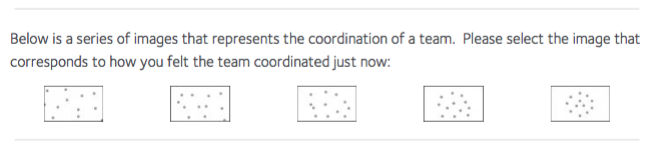
\includegraphics[width = \linewidth]{../images/teamClickPictorial.png}
  \caption{Click Pictorial Scale}
  \label{fig:clickPictorial}
\end{figure}


Due to time constraints, only the first three Click items (Unspoken Understanding, General Atmosphere, and Click Pictorial) were included in the mid-Tournament survey. The Click Pictorial measure in particular was chosen for ease of completion by athletes immediately post-game. \\

    \subsubsection{Social Bonding}

In the pre- and post-Tournament surveys, social bonding was measured using the following items:
\begin{description}
  \item [Emotional Support] ``How emotionally supportive does the team feel?''
  \item [Shared Goal] ``How strong is the feeling that everyone is working towards a shared goal?''
  \item [Group Identification Verbal] A six-item scale designed to measure an individual's personal identification with the stereotypical features of the in-group  \citep{Mael1992}.  All 6 items were measured using a 5-point Likert scale.

%1. When someone critizes my team, it feels like a personal insult
%2. I am very interested in what others think about my team
%3. When I talk about my team, I usually say “we” rather than “they"
%4. This team's successes are my successes
%5. When someone praises my team, it feels like a personal compliment
%6. If a story in the media criticized my team, I would feel embarrassed

\item [Identity Fusion Verbal] A seven-item scale designed to measure an individual's ``feeling of oneness with the group'' \citep{Swann2009}.  Identity Fusion is differentiated from Group Identification in its ability to account for an individual's felt, emotional and personal agentic associations with being a member of the target in-group \citep{Swann2012a}.  All 7 items were measured using a 5-point Likert scale.

%1. I am one with my team.
%2. I feel immersed in my team.
%3. I have a deep emotional bond with my team.
%4. My team is me.
%5. I’ll do for my team more than any of the other team members would do.
%6. I am strong because of my team.
%7. I make my team strong.

\item [Identity Fusion Pictorial] A visual scale designed to measure Identity Fusion to the target in-group \citep{Swann2009}. The pictorial scale depicts two circles, one smaller circle to denote the individual, and one larger circle to denote the group, progressively moving closer to each other such that the most ``fused'' option depicts the smaller circle encased by the larger circle. The scale offers a total of five options to chose from, see Figure ~\ref{fig:fusionPictorialGroup}.  A total of three pictorial scales were included, each with different target in-groups: team, family, and country (China).
\item [Fusion Pictorial Rank] Athletes were asked to rank their fusion to team, family, and country \citep{Whitehouse2014}.  ``Thinking about these relationships [to team, family, and country] please rank them below in order of which you feel most connected to. 1 for most connected, 3 for least connected.''
\end{description}

\begin{figure}[htbp]
  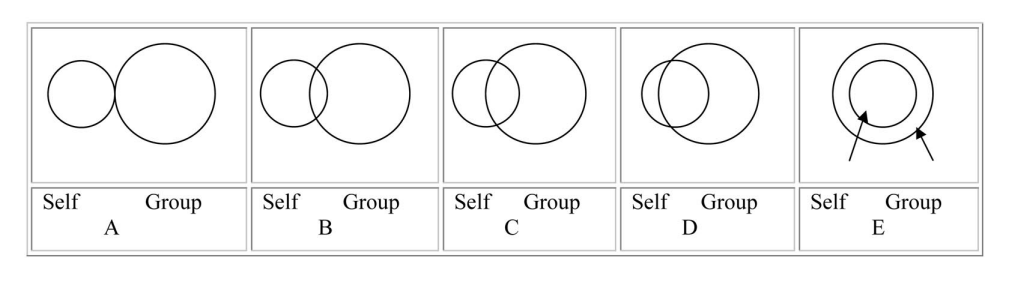
\includegraphics[width=\linewidth]{../images/Identity_Fusion_Pictorial_Scale.png}
  \caption{Identity Fusion Pictorial Scale}
  \label{fig:fusionPictorialGroup}
\end{figure}

%\insert{../images/Identity_Fusion_Pictorial_Scale.png}.

\subsubsection{Exertion, Fatigue, and Injury}
Athletes were asked to report on various components of physical and mental fatigue, exertion, and injury. First, following each mid-Tournament survey and in the post-Tournament survey, athletes were asked about their mood (``How are you feeling now after the tournament?'') and responded by choosing a point on a 10-point scale between three pairs of emotions (``Not aroused / highly aroused'',  ``Depressed/Relaxed'' and  ``Nervous/Excited'').  Many athletes experienced difficulty filling out this item in the survey, as such it was not included in the analysis. Athletes were then asked about feelings of fatigue ``How fatigued do you feel as a result of the game/tournament?'', perceived physical exertion (Borg RPE scale, \citep{Borg1990} and perceived mental exertion using two 15-point scales \citep[see][ ]{Noakes2012a}.  Finally, athletes were also asked to indicate their injury status on a 100-point scale (0 = ``Unable to play'', 100 = ``Completely fit to play'').  A baseline measure of injury was also collected in the pre-Tournament survey, but fatigue, exertion, and mood measures were excluded.

%        4.2.7
\subsubsection{Personality}
Due to the hypothesised links between personality type and dispositional tendencies towards interpersonal coordination strategies \citep{Marsh2009a}, a ten-item personality measure was included in the pre-Tournament survey \citep{Gosling2003}. Athletes were asked to indicate on a 7-point Likert scale the extent to which they agreed with 10 pairs of adjectives as appropriate descriptions of their personality (For example: ``I see myself as: dependable, self-disciplined''). Two of the ten items corresponded to one of the big-five personality types:

\begin{description}
\item [Extraversion:] 1. Extraverted, enthusiastic; 6. Reserved, quiet (Reversed scale)
\item [Agreeableness:] 2. Critical, quarrelsome (Reversed); 7. Sympathetic, warm
\item [Conscientiousness:] 3. Dependable, self-disciplined; 8. Disorganised, careless (Reversed)
\item [Emotional Stability:] 4. Anxious, easily upset (Reversed); 9. Calm, emotionally stable.
\item [Openness to Experiences:] 5. Open to new experiences, complex; 10.Conventional, uncreative (Reversed)
\end{description}


\subsection{Performance data and video data}
Following the completion of the Tournament, the CRFA provided the researcher with performance data in electronic format. These data included results for each game, minutes played and points scored by individual athletes in each game, substitutions made during each game, and video footage of every game played during the tournament. Data were stored on an encrypted external hard disk.
















\clearpage
\subsection{Procedure}

  \subsubsection{Pre-Tournament Survey}
Two months prior to the Tournament, I contacted the head coach of each provincial team and officials from the Chinese Rugby Football Association (CRFA) to seek permission for the study. \\

After receiving the permission from all participating teams and CRFA, five days prior to the Tournament I asked the coach or manager of each team to create a virtual group on We Chat containing all athletes participating in the Tournament. The WeChat group could be accessed by the athletes on their personal mobile phone devices with Internet connection. The WeChat group was populated by the coach/manager of the team, the athletes competing in the Tournament, and me. Once the WeChat group was set up, I posted a standard message in each group in which I introduced the study and provided the link to the Qualtrics survey for the athletes to complete in their own time.\\

%\begin{CJK*}{UTF8}{zhsong}
%大家好,我是前澳大利亚国家队队员,现牛津大学博士生李杰。我在做一个调查,是关于橄榄球运动员在高水平比赛前后的感受。这项研究可能有助于提升职业橄榄球运动员在高水平比赛中的表现。请所有参加河北比赛的球员完成以下的调查。
%需要大约15分钟的时间完成。您所回答的问题对于我调查信息的准确性是十分重要的,所以请如实填写问卷。调查中的所有信息仅供研究使用,并对信息进行保密。有什么关于调查的问题请直接和我联系。感谢配合! 调查链接:
%\end{CJK*}
%\url{<https://oxfordanthropology.qualtrics.com/SE/?SID=SV_7ZKXiVERWNLAKxf&Q_Language=ZH-S>}{<Qualtrics Survey>}}

\begin{quotation}
      \textit{``Hello everyone, I am former Australian 7s Representative and current Oxford University PhD candidate, Jacob Taylor (Li Jie). I am conducting a study about the experience of professional rugby players before, during and after high-level rugby competition. I hope that this research will contribute to an understanding of high-level athletic performance. Can every athlete participating in the Qianan National Tournament please complete the following survey. The survey will take about 15 minutes to complete. It is very important for the quality of the research that you answer questions honestly according to your own experiences. Survey responses are confidential and will be used for research purposes only. If you have any questions please get in touch with me. Thanks for your cooperation! Here is the survey link:''}
\end{quotation}\\
\bigskip

Upon opening the link to the survey, Athletes were asked to read a detailed brief about the survey, provide consent, and demonstrate their ability to answer the survey questions by changing the position of a virtual sliding bar that would feature in many of the survey questions. Athletes were then asked a number of questions grouped by the following categories: technical competence in rugby, feelings about the quality of recent individual and team performance, perceptions about the quality of team coordination, feelings associated with team click, social bonding, and fatigue and exertion (explained in detail below). In addition, athletes were asked to complete a ten-item personality measure (TIPI) questionnaire  \citep{Gosling2003}. The order in which each item appeared within these categories was randomised for each survey participant. At the end of the survey, athletes were asked to provide basic identification variables such as age, sex, team, position, training age, years as a member of a team, and injury status. The pre-Tournament survey took approximately 15 minutes to complete. \\

120 of a total of 174 athletes competing in the Tournament ($male = 68$, $age = 21.67$ ($SD = 3.67$, $range = 17-32$) were surveyed within a four day period before the Tournament began. Once the data collection window for the pre-Tournament survey had ceased, survey responses were collated in Qualtrics and then imported into RStudio (Version 1.0.136) for cleaning and statistical analysis. \\
%The researcher had to continually pester the athletes via friendly reminders on the WeChat group.


    \subsubsection{Mid-Tournament Surveys}

During the Tournament, athletes were surveyed following the second game of each day (or in the case of two teams, following the third game of Day 1, and the second game of Day 2).  After receiving permission from the team coach or manager, I approached each team approximately 10-20 minutes following the completion of the game, and administered a copy of the mid-Tournament survey to each athlete.  Data collection occurred on the side of the Tournament field after athletes had completed their cool-down routines. The mid-Tournament survey was similar in content to the pre-Tournament survey, but was  truncated so that athletes were able to respond quickly and without considerable disruption to their recovery from the previous game or preparation for the next game. The mid-Tournament took approximately 3 minutes complete. Completed surveys were collected by the researcher and sealed in envelopes labelled by team.  Survey responses were later manually collated and data were imputed into a .csv file using Microsoft Excel (Version 14.7.1). Collated data were then combined with other survey and performance data to be analysed in RStudio. \\


        \subsubsection{Post-Tournament Survey}

The post-Tournament survey was administered via the same WeChat group that was set up for the pre-Tournament survey. Data collection for the post-Tournament survey began the day after the completion of the Tournament, and finished four days following the Tournament. Athletes were asked to respond to questions relating to individual and team performance, joint-action, social bonding, fatigue and exertion, framed in terms of their experience of the Tournament as a whole. Survey responses were collated in Qualtrics and then imported into RStudio, where they were cleaned and merged with pre-Tournament and mid-Tournament survey responses for statistical analysis.


        \subsubsection{Tournament performance data}
Following the completion of the Tournament, game-by-game information (game result, points scored, starting team, substitutions made, etc.) was collected from the CRFA Tournament statistician. These data were manually imputed into a data frame in Microsoft Excel, before being imported as a .csv file into RStudio to be merged with other data (pre-tournament survey, mid-Tournament surveys, post-Tournament surveys, and post-Tournament survey) for statistical analysis.


\subsection{Data Structure}
Overall, data were collected on 174 unique athletes at eight different time points: once pre-Tournament, six times during the tournament (once per game), and once post-Tournament. Survey responses were recorded for a total of 165 unique athletes at four different time points: once pre-Tournament, twice during the tournament, and once post-Tournament. Table ~\ref{tab:tournamentData}

      \begin{table}[htbp]\caption{Data collected during the Tournament}
        \begin{center}
          \begin{small}
            \begin{tabular}{r r r r}
                Time & Phase & Survey Data (Men) & Performance Data (Men) \\
                \hline\hline
                1 & pre-Tournament & \bf 120 (68) & - \\
                2 & Game 1 & - & 174 (68) \\
                3 & Game 2 & \bf129 (60) & 174 (93) \\
                4 & Game 3 & \bf22 (8) & 174 (93) \\
                \hline
                5 & Game 4 & - & 174 (68) \\
                6 & Game 5 & \bf 163 (91) & 174 (93) \\
                7 & Game 6 & - & 174 (68) \\
                8 & post-Tournament & \bf118 (93) & - \\
            \end{tabular}
          \end{small}
        \end{center}
        \label{tab:tournamentData}
      \end{table}

On Day 1 of the Tournament, 129 athletes in 11 teams were surveyed after their 2nd game of the day, 22 athletes in 2 teams were surveyed after their 3rd game. 2 of 11 teams (Hebei men’s and Fujian men’s) were not surveyed due to timing and logistical constraints experienced by the researcher during data collection. On Day 2 of the Tournament, 163 athletes in 14 teams were surveyed after their second game of the day. One team (Shanghai Women’s) was not surveyed due to timing and logistical constraints experienced by the researcher. The challenges of data collection meant that observations were missing for athletes across the four survey time points. Missingness in the survey data ranged from 15-19\% at any one of the four survey time points.\\

%      4.2


































\clearpage
\section{Analysis}


\subsection{Overview of Analysis}

Predictions of this study were tested by analysing the collected data in three steps:\\

\begin{enumerate}
  \item A focussed analysis of the \textbf{post-Tournament} survey responses
  \item An analysis of \textit{changes} in variables between \textbf{pre- and post-Tournament} responses
  \item Analysis of the relationship between team performance, team click, and social bonding (fatigue) in survey data over the \textbf{entire Tournament}.
\end{enumerate}

Analysis of data collected following the Tournament (phase 1) would provide an indication of the effects of a high-intensity, high stakes professional Tournament. Was there a statistically meaningful relationship between perceived team performance, team click, and social bonding in response to athlete experience of the Tournament? Subsequently, investigating the extent to which athlete responses changed as a result of the Tournament could provide confirmatory evidence for study predictions. Can pre- to post-Tournament changes in outcome variables (team click, social bonding, and fatigue) be explained by pre-post Tournament variation in perceptions of joint-action success and feelings of team click? Third, analysis of the entire survey data set, including the mid-Tournament survey responses, allowed for a more thorough assessment of the consistency of a hypothesised relationship between joint-action success, team click, and social bonding. Mid-Tournament surveys were administered in-situ and in the moment, and were therefore less susceptible to desirability bias and pre/post-hoc rationalisations by athletes. By analysing multiple observations for the same athlete over a number of time points, it was possible to better account for intra- and inter-individual variation, and therefore enables more robust statistical inferences.









\subsection{Analysis of post-Tournament data}


\subsubsection{post-Tournament Descriptive Statistics}

118 (male = 65) out of a total of 174 athletes who participated in the Tournament completed the post-Tournament survey. Athletes completing the pre- and post-Tournament surveys were not subject to time constraints, and so the full compliment of survey items for each category of variables outlined in the methods section (performance, click, bonding, and fatigue) were included. In addition to these survey responses, Tournament performance measures provided by CRFA, and measures of technical competence and other identification variables provided in the pre-Tournament survey were used to supplement analysis of the post-Tournament data. Summary statistics for each category of survey variables are outlined in Tables below.

\begin{table}[htpb]\caption{Summary Statistics: post-Tournament Technical Competence (objective and subjective)}
\begin{center}
\begin{small} 
\begin{tabular}
{l
r
r
r
r
r
r
r
}

\multicolumn{
7
}{l}{

}
\cr 
 \hline 
Variable  &  
n  & 
mean  & 
sd  & 
min  & 
max  & 
skew  & 
krtss \cr 

 \hline 

Years In Team   &  120  &   3.17  &   2.12  &    0  &   7  &   0.29  &  -1.25 \cr 

Training Age   &  120  &   4.40  &   2.35  &    0  &  13  &   0.47  &   0.66 \cr 

Starting Team Average   &  172  &   0.61  &   0.36  &    0  &   1  &  -0.43  &  -1.32 \cr 

Age   &  121  &  21.67  &   3.26  &   16  &  32  &   0.52  &  -0.27 \cr 

Ability Teammates   &  120  &  19.45  &  20.14  &  -40  &  50  &  -0.31  &  -0.56 \cr 

Ability Chinese Pros   &  120  &  15.78  &  19.59  &  -35  &  50  &  -0.18  &  -0.65 \cr 

Ability International   &  120  &  18.46  &  26.19  &  -44  &  50  &  -0.48  &  -0.77 \cr 

Team Ability China   &  120  &  22.48  &  22.90  &  -40  &  50  &  -0.64  &  -0.58 \cr 

 \hline 
\end{tabular}
\end{small}
\end{center}
\label{tab:1competenceDescriptives}
\end{table} 



\begin{table}[htpb]\caption{Summary Statistics: post-Tournament Performance (individual and team)}
\begin{center}
\begin{small} 
\begin{tabular}
{l
r
r
r
r
r
r
r
}

\multicolumn{
7
}{l}{

}
\cr 
 \hline 
Variable  &  
{n} & 
{mean} & 
{sd} & 
{min} & 
{max} & 
{skew} & 
{krtss}\cr 

 \hline 

indPerformance7   &  118  &  56.36  &  23.47  &  0  &  100  &  -0.35  &  -0.08 \cr 

passingTech7   &  118  &  58.41  &  24.25  &  0  &  100  &  -0.79  &   0.05 \cr 

supportAttack7   &  118  &  62.62  &  22.70  &  0  &  100  &  -0.98  &   0.64 \cr 

indDefense7   &  118  &  57.64  &  23.57  &  0  &  100  &  -0.55  &  -0.11 \cr 

effectContact7   &  118  &  62.15  &  24.81  &  0  &  100  &  -0.97  &   0.40 \cr 

decisionAttack7   &  118  &  61.22  &  21.43  &  0  &  100  &  -0.72  &   0.37 \cr 

teamPerformance7   &  118  &  64.36  &  23.61  &  0  &  100  &  -0.52  &  -0.30 \cr 

teamDefense7   &  118  &  62.42  &  22.50  &  0  &  100  &  -0.52  &  -0.52 \cr 

teamAttack7   &  118  &  65.33  &  20.26  &  0  &  100  &  -0.53  &  -0.23 \cr 

teamSupportPlay7   &  118  &  65.75  &  19.72  &  0  &  100  &  -0.76  &   0.57 \cr 

teamCommunication7   &  118  &  65.25  &  21.26  &  0  &  100  &  -0.65  &   0.27 \cr 

 \hline 
\end{tabular}
\end{small}
\end{center}
\label{tab:2performancePostDescriptives}
\end{table} 



\begin{table}[htpb]\caption{Summary Statistics: post-Tournament Team Click}
\begin{center}
\begin{small} 
\begin{tabular}
{l
r
r
r
r
r
r
r
}

\multicolumn{
7
}{l}{

}
\cr 
 \hline 
Variable  &  
{n} & 
{mean} & 
{sd} & 
{min} & 
{max} & 
{skew} & 
{krtss}\cr 

 \hline 

unspokenUnderstanding7   &  118  &  72.72  &  19.95  &  0  &  100  &  -1.38  &  2.13 \cr 

generalAtmosphere7   &  118  &  78.45  &  21.34  &  0  &  100  &  -1.51  &  2.82 \cr 

clickPictorial7   &  118  &   3.93  &   1.04  &  1  &    5  &  -0.78  &  0.00 \cr 

reliabilityOfOthers7   &  118  &  68.00  &  23.09  &  0  &  100  &  -1.33  &  1.75 \cr 

reliabilityForOthers7   &  118  &  63.45  &  25.80  &  0  &  100  &  -1.06  &  0.51 \cr 

abilityExtended7   &  118  &  72.25  &  19.27  &  0  &  100  &  -1.13  &  2.03 \cr 

 \hline 
\end{tabular}
\end{small}
\end{center}
\label{tab:3clickPostDescriptives}
\end{table} 



\begin{table}[htpb]\caption{Summary Statistics: post-Tournament Social Bonding}
\begin{center}
\begin{small} 
\begin{tabular}
{l
r
r
r
r
r
r
r
}

\multicolumn{
7
}{l}{

}
\cr 
 \hline 
Variable  &  
{n} & 
{mean} & 
{sd} & 
{min} & 
{max} & 
{skew} & 
{krtss}\cr 

 \hline 

emotionalSupport7   &  118  &  79.67  &  18.84  &   0.00  &  100  &  -1.74  &  4.37 \cr 

sharedGoal7   &  118  &  86.00  &  15.56  &  29.00  &  100  &  -1.38  &  2.24 \cr 

groupId7   &  118  &   4.29  &   0.67  &   1.50  &    5  &  -1.18  &  1.66 \cr 

fusionVerbal7   &  118  &   4.00  &   0.71  &   1.43  &    5  &  -0.86  &  0.99 \cr 

fusionPictorialTeam7   &  118  &   4.33  &   1.19  &   0.00  &    5  &  -2.45  &  6.07 \cr 

fusionPictorialFamily7   &  118  &   4.51  &   0.96  &   0.00  &    5  &  -2.30  &  5.62 \cr 

fusionPictorialCountry7   &  118  &   4.03  &   1.39  &   0.00  &    5  &  -1.59  &  1.84 \cr 

 \hline 
\end{tabular}
\end{small}
\end{center}
\label{tab:4bondingPostDescriptives}
\end{table} 



\begin{table}[htpb]\caption{Summary Statistics: post-Tournament measures of fatigue}
\begin{center}
\begin{small} 
\begin{tabular}
{l
r
r
r
r
r
r
r
}

\multicolumn{
7
}{l}{

}
\cr 
 \hline 
Variable  &  
n  & 
mean  & 
sd  & 
min  & 
max  & 
skew  & 
krtss \cr 

 \hline 

Fatigue   &  118  &  69.27  &  21.24  &   0  &  100  &  -1.13  &  1.40 \cr 

RPE(physical)   &  118  &  14.97  &   2.66  &   6  &   20  &  -0.80  &  0.49 \cr 

RPE(mental)   &  118  &   6.08  &   2.47  &  -4  &   10  &  -1.13  &  1.82 \cr 

injuryRev7   &  118  &  23.86  &  26.91  &   0  &  100  &   1.19  &  0.60 \cr 

 \hline 
\end{tabular}
\end{small}
\end{center}
\label{tab:5fatiguePostDescriptives}
\end{table} 



\begin{table}[htpb]\caption{Summary Statistics: Objective Tournament Performance}
\begin{center}
\begin{small} 
\begin{tabular}
{l
r
r
r
r
r
r
r
}

\multicolumn{
7
}{l}{

}
\cr 
 \hline 
Variable  &  
n  & 
mean  & 
sd  & 
min  & 
max  & 
skew  & 
krtss \cr 

 \hline 

Final Rank   &  174  &   4.83  &   2.15  &   1  &   8  &  -0.09  &  -1.17 \cr 

Wins - Losses   &  172  &   0.32  &   2.94  &  -6  &   6  &  -0.17  &  -0.25 \cr 

Total Ind Points   &  172  &   8.45  &  11.41  &   0  &  69  &   2.34  &   7.23 \cr 

Total Ind Minutes   &  172  &  44.01  &  20.65  &   1  &  81  &  -0.38  &  -0.89 \cr 

Starting Team Avg   &  172  &   0.61  &   0.36  &   0  &   1  &  -0.43  &  -1.32 \cr 

 \hline 
\end{tabular}
\end{small}
\end{center}
\label{tab:6objectiveTournamentDescriptives}
\end{table} 




\clearpage

\subsubsection{Data Reduction using Exploratory Factor Analysis}

Before attempting to make any statistical inferences, data reduction was required in order to make analyses more tractable and parsimonious. Data reduction allows for a reduction in multicollinearity between predictor variables of interest while retaining as much variance as possible in the observed data \citep{Yong2013}. Second, certain data reduction techniques are also capable of representing the underlying theoretical structure of the collected data. Given that the survey items of this study were designed to collectively access more latent psychological constructs, particularly in the case of outcome variables related to concepts such as team click, social bonding, and fatigue (but also for performance variables), a data reduction technique capable modelling the theoretical structure of these data was preferred.

Exploratory Factor Analysis (EFA) was therefore the most suitable data reduction technique for the purposes of this study. EFA is one of various available data reduction techniques, and is distinct from its main alternative, Principal Components Analysis (PCA), in that it is capable of modelling the latent dimensions of a collection of variables.\footnote{PCA is concerned only with establishing which components exist within the existing data and how a particular variable might contribute that component. To do this, PCA makes the assumption that all variance in a subset of variables is common variance, and therefore communality between all variables is equal to 1. From this assumption, the original data can be transposed into a linear model without the need for a communality-dependent estimated coefficient for each variable\citep{Widaman2007}. EFA examines all the pairwise relationships between individual variables and seeks to extract latent factors from the measured variables. By using Squared Multiple Correlations (which are essentially multiple regressions in which each variable is predicted by all others) to calculate the common variance (communality) between each variable in an analysis (the communality value is much like an R-squared value from a multiple regression). The square root of the communality score for each variable is then used as a coefficient that conditions the relationship between each variable and the underlying dimensions (factors) identifiable in the data. Also known as ``factor loadings,'' these coefficients become the parameters of linear model capable of estimating factor scores for each individual observation, which can be utilised in subsequent statistical analysis in place of single variable observations.\\

A final step in the EFA procedure is the process of ``rotation'', which is an optimisation technique designed to encourage each variable to load on as few factors as possible \citep{Rummel1988}. Rotation refers to a geometric conception of factor analysis, in which individual variables can be plotted in n-dimensional space according to their relationship to each dimension (or factor). By rotating the axes of these dimensions, the distance of a given variable to that dimension (factor) can be reduced, which results in an increase in factor loading on one factor and (ideally) a decrease in factor loading on another uncorrelated variable. Orthogonal (or perpendicular) rotation of axes refers to axes, say X and Y, maintaining a 90-degree perpendicularity and rotating clockwise or anticlockwise, depending on the location of the variable clusters. Orthogonal rotation thus enables optimisation of loadings for clusters of variables that are distant from each other in n-dimensional space. If correlation exists between clusters of variables, however, rotating axes obliquely (inwards towards each other) provides a more effective way of reducing the distance between clusters of variables and the latent dimensions that account for such clustering Osborne2015. See Figure ~\ref{fig:orthogonalOblique} for a graphical  illustration of the difference between orthogonal and oblique rotation. Given that most variables of interest in the present study were at least mildly correlated, I opted for an oblique rotation method. Subsequent EFAs were conducted using the factanal() function in the Stats package (Version 3.3.0) in R, using the ``promax'' (oblique) rotation method (Gorsuch, 1983). Factor scores were scores were approximately zero-centred, with a standard deviation of approximately 1 (standardised z-scores).

\begin{figure}[htbp]
  \begin{center}
    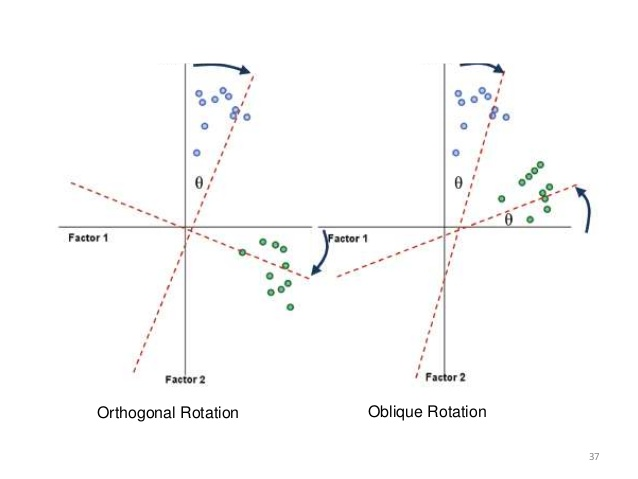
\includegraphics[width= \linewidth, scale = .5]{../images/orthogonalObliqueRotationExample.jpg}
    \caption{Orthogonal and oblique rotation methods}
    \label{fig:orthogonalOblique}
  \end{center}
\end{figure}

\subsubsection{Assessment of EFA}
EFA’s were assessed using the following criteria. Prior to factors being extracted, correlation matrices were subjected to two common sampling adequacy measures: the Kaiser-Meyer-Olkin (KMO) index and Bartlett’s test of sphericity. The KMO index provides a proportion measure of common variance to partial correlations among examined variables\footnote{If the KMO index is high ($\approx$ 1), the EFA can act efficiently; if KMO is low ($\approx$ 0), the proposed EFA is not suitable for analysis.} while Bartlett’s test of sphericity is used to test the null hypothesis that the correlation matrix is an identity matrix (i.e., a square matrix in which all the elements of the principal diagonal are equal to 1, and all other elements are 0s). Factor loadings of $> .3$ were considered adequate, and only items that loaded on one factor were accepted \citep{Field2012}. Finally, two reliability measures (Guttman's lambda3 and Cronbach's Alpha were also reported to suggest whether or not the average correlation of each subset of variables is an accurate estimate of the average correlation of all items that could pertain to the underlying construct.\footnote{Cronbach's $\alpha$ is a function of the number of items in a test, the average covariance between item-pairs, and the variance of the total score \citep{Tabachnick2007}}. Eigenvalues, or Sum of Squares Loadings (SS Loadings) for each factor were also reported\citep{Dziuban1974}.





\subsubsection{EFA of post-Tournament Variables}

\myparagraph{Technical Competence}
All eight items relevant to technical competence were analysed in a correlation matrix to assess relatedness (see Table ~\ref{tab:1competenceCorr}). Medium correlations among measures of objective competence (three out of four items correlated at $> .3$) and among measures of subjective competence (all items except for team competence measure correlated at $> .3$) suggested that the data could be explained by two underlying factors. Team Ability Chinese Provinces was dropped from analysis due to low correlation with other competence variables, and because the item did not ask about an individual athlete’s competence (it referred instead to an athlete’s opinion of the competence of the team of which they were a member). An examination of the KMO measure of sampling adequacy ($KMO = .67$), and the Bartlett sphericity test indicated that two factors were adequate, $\chi^2(21, N = 120) = 239.71$, $p < .001$. \\


An EFA (with oblique ``promax'' rotation) of technical competence variables revealed that items of interest loaded on two factors. The exception was the variable starting Reserve, which failed to load on either factor, and was thus dropped from analysis. Measures of objective competence (Years Team, Training Age, and Age) loaded on the first factor, which was labelled ``Objective Competence'' because the measures were all objective markers of an athlete's competence.  Objective Competence explained 26.4\% of the total variance ($SS Loading = 1.85$). The remaining measures of subjective competence (Ability Teammates, Ability Chinese Pros, Ability International Pros) loaded on the remaining factor.  The second factor was labelled ``Subjective Competence'', due to the fact that all measures were the product of athlete self-report.  Subjective competence explained 23.8\% of the variance ($SS Loading = 1.67$). $Guttman's \lambda =.74$ and $Cronbach's \alpha = (.67)$ indicated that the data reduction was appropriate and reliable.



\myparagraph{Component Performance for Individual and Team}
First, items related to athlete perception of components of performance were isolated from overall perceptions of performance relative to prior individual expectations for further data reduction. Given that the theoretical predictions of this dissertation concentrate in particular on athlete perceptions of joint-action, individual and team components of performance were analysed, with the intention that perceptions of success in individual performance components would be used as a statistical control for perceptions of joint-action success.

Items concerning team component performance (team defence, team attack, team support play, and on field communication) were subjected to EFA.  Correlations between team component performance items was very high (all $r's > .5$), which suggested that one factor would be appropriate (see Table ~\ref{tab:22teamPerformancePostCorr}). The KMO index and Bartlett's test both suggested high sampling adequacy, ($KMO = 0.79$, $\chi^2(6, N = 118) = 342.14$, $p < .001$).  One factor, labelled ``Joint Action Success'' was imposed on the data, which explained 72.8\% of the overall variance (SS Loading = 2.91). $Guttman's \lambda =.90$ and $Cronbach's \alpha = .91$ indicated that the data reduction was appropriate and reliable.

%, $\chi^2 (df=2) = 14.81$, $p < .001$,

Items relating to individual component performance (passing technique, support play in attack, 1on1 defence, and decision making in attack) were subjected to an EFA.  Correlations between individual component performance items were also very high (all $r's > .5$, see Table ~\ref{tab:21indPerformancePostCorr}), which suggested that one factor would be sufficient (confirmed by $KMO =  0.84$, corrtest Bartlett: $\chi^2(10, N = 118) =  326.38$, $p < .001$).  One factor was extracted and labelled ``Ind Performance Success'', which explained 62.1\% of the overall variance (SS Loading = 3.10) .  $Guttman's \lambda =.88$ and $Cronbach's \alpha = .89$ both indicated that the data reduction was appropriate.
%$\chi^2 (df=5) = 15.47$, $p < .01$

To confirm that the theoretically motivated separation of Joint Action Success from Ind Performance Success was appropriate for the collected data, a follow up EFA was conducted, in which team and individual performance component variables were combined in one matrix. Sampling adequacy measures indicated high suitability ($KMO = 0.83$, $\chi^2(36, N = 118) = 726.60$, $p < .0001$).  As expected, an EFA extracted two factors, with Individual performance measures loaded on one factor (proportion of variance = .34, $SS Loading = 3.09$), and team performance measures loading on a second factor (proportion of variance = .32, $SS Loading = 2.90$). $Guttman's \lambda =.93$ and $Cronbach's \alpha = .90$ indicated that the data reduction was appropriate.


\myparagraph{Team Click}
Next, EFA was performed on post-Tournament variables associated with team click. Strong correlations between all variables of interest ($r's > .3$, see Table ~\ref{tab:3clickPostCorr}) and sampling adequacy measures suggested that imposing one factor was appropriate, $KMO =  0.69$, $\chi^2(15, N = 118) = 182.73$, $p < .001$.  One factor labelled ``Team Click'' was extracted from the data, which explained 34.5\% of the overall variance ($SS Loading = 2.07$).  Guttman's $\lambda =.76$ and Cronbach's $\alpha = .75$ indicated that the data reduction was appropriate.
%, and a Chi-squared test indicated that one factor was sufficient to account for the variance of these items ($\chi^2 (9, ) = 46.36$, $p < .001$).

%Interestingly, when click and bonding measures were analysed together, the following loading were observed:
%Loadings:
%                       Factor1 Factor2
%unspokenUnderstanding7  0.710
%generalAtmosphere7      0.713
%clickPictorial7         0.672  -0.106
%reliabilityOfOthers7    0.128   0.539
%reliabilityForOthers7           0.424
%abilityExtended7       -0.110   0.956
%emotionalSupport7       0.656   0.131
%sharedGoal7             0.838
%fusionPictorialTeam7    0.424
%fusionVerbal7           0.138   0.281


\myparagraph{Social Bonding}
Survey items related to feelings of social bonding (to team) were separately analysed for the purposes of data reduction. A correlation matrix (~\ref{tab:4bondingPostCorr}) indicated that Group Identification did not share common variance with other variables (all correlations were $<.1$, except for the verbal measures of Identity Fusion ($r =.358$)). As such,  Group Identification was excluded from analysis.  Sampling adequacy variables suggested that the remaining subset of variables were appropriate for analysis, $KMO = 0.65$, $\chi^2(10, N = 118) = 108.22$, $p < .001$.  EFA was performed on 4 remaining items, imposing one factor labelled ``Social Bonding'', which explained 34.5\% of the overall variance ($SS Loading = 1.60$, $Guttman's \lambda =.66$ and $Cronbach's \alpha = .65$).

\myparagraph{Fatigue}
Finally, post-Tournament survey items relating to perceptions of fatigue and exertion were separately analysed for the purposes of data reduction.  Due to difficulty completing questions related to arousal in the online and in-person surveys, mood-related items were excluded from analysis.  In addition, it was clear from correlation values that injury status did not strongly correlate with other items relevant to fatigue and exertion, and was therefore also excluded from subsequent analysis (see Table ~\ref{tab:5fatiguePostCorr}).  The KMO index and Bartlett's test of sphericity indicated that the remaining subset of variables was appropriate for EFA, $KMO =  0.69$, $\chi^2(3, N = 118) = 111.93$, $p < .001$. EFA was performed on 3 remaining items (fatigue, physical perceived exertion, and mental perceived exertion), which imposed one factor labelled ``fatigue.''  The extracted factor explained 57.8\% of the overall variance (SS Loadings = 1.7, $Guttman's\lambda =.73$ and Cronbach's $\alpha = .80$).

Summary statistics for the factors extracted from the post-Tournament data, and their correlations can be viewed in Table ~\ref{tab:postTournamentFactorDescriptives} and Table ~\ref{tab:postTournamentFactorCorr} respectively.

\newpage
\newgeometry{margin=0.5cm} % modify this if you need even more space
\begin{landscape}


% Table created by stargazer v.5.2.2 by Marek Hlavac, Harvard University. E-mail: hlavac at fas.harvard.edu
% Date and time: Mon, Aug 27, 2018 - 18:51:00
\begin{table}[!htbp] \centering 
  \caption{Correlation Matrix: post-Tournament Technical Competence} 
  \label{tab:1competenceCorr} 
\scriptsize 
\begin{tabular}{@{\extracolsep{5pt}} ccccccccc} 
\\[-1.8ex]\hline 
\hline \\[-1.8ex] 
 & Years In Team & Training Age & Starting Team Average & Age & Ability Teammates & Ability Chinese Pros & Ability International & Team Ability China \\ 
\hline \\[-1.8ex] 
Years In Team & $1$ & $0.510$ & $$-$0.044$ & $0.569$ & $0.076$ & $0.102$ & $0.099$ & $0.261$ \\ 
Training Age & $0.510$ & $1$ & $0.0004$ & $0.697$ & $0.095$ & $0.183$ & $0.201$ & $0.190$ \\ 
Starting Team Average & $$-$0.044$ & $0.0004$ & $1$ & $$-$0.040$ & $0.203$ & $0.099$ & $0.044$ & $0.144$ \\ 
Age & $0.569$ & $0.697$ & $$-$0.040$ & $1$ & $0.132$ & $0.089$ & $0.154$ & $0.212$ \\ 
Ability Teammates & $0.076$ & $0.095$ & $0.203$ & $0.132$ & $1$ & $0.428$ & $0.383$ & $0.454$ \\ 
Ability Chinese Pros & $0.102$ & $0.183$ & $0.099$ & $0.089$ & $0.428$ & $1$ & $0.702$ & $0.273$ \\ 
Ability International & $0.099$ & $0.201$ & $0.044$ & $0.154$ & $0.383$ & $0.702$ & $1$ & $0.212$ \\ 
Team Ability China & $0.261$ & $0.190$ & $0.144$ & $0.212$ & $0.454$ & $0.273$ & $0.212$ & $1$ \\ 
\hline \\[-1.8ex] 
\end{tabular} 
\end{table} 


% Table created by stargazer v.5.2 by Marek Hlavac, Harvard University. E-mail: hlavac at fas.harvard.edu
% Date and time: Sun, Jun 25, 2017 - 21:08:16
\begin{table}[!htbp] \centering 
  \caption{Correlation Matrix: post-Tournament Team Performance} 
  \label{tab:22teamPerformancePostCorr} 
\footnotesize 
\begin{tabular}{@{\extracolsep{5pt}} ccccc} 
\\[-1.8ex]\hline 
\hline \\[-1.8ex] 
 & Team Defence & Team Attack & Team Support Play & Team Onfield Communication \\ 
\hline \\[-1.8ex] 
Team Defence & $1$ & $0.834$ & $0.643$ & $0.721$ \\ 
Team Attack & $0.834$ & $1$ & $0.740$ & $0.713$ \\ 
Team Support Play & $0.643$ & $0.740$ & $1$ & $0.715$ \\ 
Team Onfield Communication & $0.721$ & $0.713$ & $0.715$ & $1$ \\ 
\hline \\[-1.8ex] 
\end{tabular} 
\end{table} 


% Table created by stargazer v.5.2 by Marek Hlavac, Harvard University. E-mail: hlavac at fas.harvard.edu
% Date and time: Sun, Jun 25, 2017 - 21:07:58
\begin{table}[!htbp] \centering 
  \caption{Correlation Matrix: Individual Performance} 
  \label{tab:21indPerformancePostCorr} 
\footnotesize 
\begin{tabular}{@{\extracolsep{5pt}} cccccc} 
\\[-1.8ex]\hline 
\hline \\[-1.8ex] 
 & Passing Tech & Support In Attack & Ind Defence & Effectiveness In Contact & Decision Making Attack \\ 
\hline \\[-1.8ex] 
Passing Tech & $1$ & $0.658$ & $0.510$ & $0.508$ & $0.607$ \\ 
Support In Attack & $0.658$ & $1$ & $0.658$ & $0.641$ & $0.734$ \\ 
Ind Defence & $0.510$ & $0.658$ & $1$ & $0.590$ & $0.525$ \\ 
Effectiveness In Contact & $0.508$ & $0.641$ & $0.590$ & $1$ & $0.713$ \\ 
Decision Making Attack & $0.607$ & $0.734$ & $0.525$ & $0.713$ & $1$ \\ 
\hline \\[-1.8ex] 
\end{tabular} 
\end{table} 


% Table created by stargazer v.5.2.2 by Marek Hlavac, Harvard University. E-mail: hlavac at fas.harvard.edu
% Date and time: Mon, Aug 27, 2018 - 18:51:00
\begin{table}[!htbp] \centering 
  \caption{Correlation Matrix: post-Tournament Team Click} 
  \label{} 
\footnotesize 
\begin{tabular}{@{\extracolsep{5pt}} ccccccc} 
\\[-1.8ex]\hline 
\hline \\[-1.8ex] 
 & unspokenUnderstanding7 & generalAtmosphere7 & clickPictorial7 & reliabilityOfOthers7 & reliabilityForOthers7 & abilityExtended7 \\ 
\hline \\[-1.8ex] 
unspokenUnderstanding7 & $1$ & $0.626$ & $0.508$ & $0.275$ & $0.230$ & $0.375$ \\ 
generalAtmosphere7 & $0.626$ & $1$ & $0.385$ & $0.301$ & $0.276$ & $0.265$ \\ 
clickPictorial7 & $0.508$ & $0.385$ & $1$ & $0.282$ & $0.021$ & $0.213$ \\ 
reliabilityOfOthers7 & $0.275$ & $0.301$ & $0.282$ & $1$ & $0.276$ & $0.544$ \\ 
reliabilityForOthers7 & $0.230$ & $0.276$ & $0.021$ & $0.276$ & $1$ & $0.375$ \\ 
abilityExtended7 & $0.375$ & $0.265$ & $0.213$ & $0.544$ & $0.375$ & $1$ \\ 
\hline \\[-1.8ex] 
\end{tabular} 
\end{table} 


\clearpage

% Table created by stargazer v.5.2 by Marek Hlavac, Harvard University. E-mail: hlavac at fas.harvard.edu
% Date and time: Tue, May 30, 2017 - 09:19:43
\begin{table}[!htbp] \centering 
  \caption{Correlation Matrix: post-Tournament Social Bonding} 
  \label{} 
\footnotesize 
\begin{tabular}{@{\extracolsep{5pt}} cccccc} 
\\[-1.8ex]\hline 
\hline \\[-1.8ex] 
 & emotionalSupport & sharedGoal & groupIdentification & identityFusionVerbal & identityFusionPictorialTeam \\ 
\hline \\[-1.8ex] 
emotionalSupport & $1$ & $0.619$ & $0.079$ & $0.331$ & $0.349$ \\ 
sharedGoal & $0.619$ & $1$ & $0.061$ & $0.246$ & $0.395$ \\ 
groupIdentification & $0.079$ & $0.061$ & $1$ & $0.358$ & $0.081$ \\ 
identityFusionVerbal & $0.331$ & $0.246$ & $0.358$ & $1$ & $0.220$ \\ 
identityFusionPictorialTeam & $0.349$ & $0.395$ & $0.081$ & $0.220$ & $1$ \\ 
\hline \\[-1.8ex] 
\end{tabular} 
\end{table} 


% Table created by stargazer v.5.2 by Marek Hlavac, Harvard University. E-mail: hlavac at fas.harvard.edu
% Date and time: Sat, Jun 03, 2017 - 22:22:24
\begin{table}[!htbp] \centering 
  \caption{Correlation Matrix: post-Tournament Fatigue} 
  \label{} 
\footnotesize 
\begin{tabular}{@{\extracolsep{5pt}} ccccc} 
\\[-1.8ex]\hline 
\hline \\[-1.8ex] 
 & fatigue & RPE(physical) & RPE(mental) & injuryRev7 \\ 
\hline \\[-1.8ex] 
fatigue & $1$ & $0.665$ & $0.510$ & $0.090$ \\ 
RPE(physical) & $0.665$ & $1$ & $0.523$ & $0.009$ \\ 
RPE(mental) & $0.510$ & $0.523$ & $1$ & $$-$0.040$ \\ 
injuryRev7 & $0.090$ & $0.009$ & $$-$0.040$ & $1$ \\ 
\hline \\[-1.8ex] 
\end{tabular} 
\end{table} 


% Table created by stargazer v.5.2 by Marek Hlavac, Harvard University. E-mail: hlavac at fas.harvard.edu
% Date and time: Tue, May 30, 2017 - 09:19:44
\begin{table}[!htbp] \centering 
  \caption{Tournament Performance Correlation Matrix} 
  \label{} 
\footnotesize 
\begin{tabular}{@{\extracolsep{5pt}} cccccc} 
\\[-1.8ex]\hline 
\hline \\[-1.8ex] 
 & finalRank & totalWins - totalLosses & totalIndPoints & totalMinutesPlayed & startingTeamAvg \\ 
\hline \\[-1.8ex] 
finalRank & $1$ & $0.901$ & $0.381$ & $0.062$ & $0.055$ \\ 
totalWins - totalLosses & $0.901$ & $1$ & $0.428$ & $0.129$ & $0.089$ \\ 
totalIndPoints & $0.381$ & $0.428$ & $1$ & $0.404$ & $0.067$ \\ 
totalMinutesPlayed & $0.062$ & $0.129$ & $0.404$ & $1$ & $$-$0.038$ \\ 
startingTeamAvg & $0.055$ & $0.089$ & $0.067$ & $$-$0.038$ & $1$ \\ 
\hline \\[-1.8ex] 
\end{tabular} 
\end{table} 


\clearpage
\begin{table}[htpb]\caption{Summary Statistics: post-Tournament Factors}
\begin{center}
\begin{scriptsize} 
\begin{tabular}
{l
r
r
r
r
r
r
r
}

\multicolumn{
7
}{l}{

}
\cr 
 \hline 
Variable  &  
n  & 
mean  & 
sd  & 
min  & 
max  & 
skew  & 
krtss \cr 

 \hline 

objCompetence   &  120  &   0.00  &   0.95  &  -1.99  &    2.91  &   0.45  &  -0.23 \cr 

subjCompetence   &  120  &   0.00  &   0.96  &  -2.58  &    1.79  &  -0.16  &  -0.66 \cr 

indPerformExp   &  118  &  56.36  &  23.47  &   0.00  &  100.00  &  -0.35  &  -0.08 \cr 

indPerformSuccess   &  118  &   0.00  &   0.95  &  -2.96  &    1.70  &  -0.85  &   0.60 \cr 

teamPerformanceExpect   &  118  &  64.36  &  23.61  &   0.00  &  100.00  &  -0.52  &  -0.30 \cr 

jointActionSuccess   &  118  &   0.00  &   0.96  &  -3.28  &    1.79  &  -0.49  &  -0.01 \cr 

teamClick   &  118  &   0.00  &   0.90  &  -3.06  &    1.42  &  -1.01  &   1.03 \cr 

socialBonding   &  118  &   0.00  &   0.89  &  -3.08  &    1.08  &  -1.38  &   2.00 \cr 

fatigue   &  118  &   0.00  &   0.91  &  -3.40  &    1.67  &  -1.03  &   1.56 \cr 

 \hline 
\end{tabular}
\end{scriptsize}
\end{center}
\label{tab:postTournamentFactorDescriptives}
\end{table} 




% Table created by stargazer v.5.2.2 by Marek Hlavac, Harvard University. E-mail: hlavac at fas.harvard.edu
% Date and time: Mon, Aug 27, 2018 - 18:51:01
\begin{table}[!htbp] \centering 
  \caption{post-Tournament Factors Correlation Matrix} 
  \label{tab:postTournamentFactorCorr} 
\scriptsize 
\begin{tabular}{@{\extracolsep{5pt}} cccccccccc} 
\\[-1.8ex]\hline 
\hline \\[-1.8ex] 
 & objCompetence & subjCompetence & indPerformExp & indPerformSuccess & teamPerformanceExpect & jointActionSuccess & teamClick & socialBonding & fatigue \\ 
\hline \\[-1.8ex] 
objCompetence & $1$ & $$-$0.146$ & $0.065$ & $0.319$ & $$-$0.128$ & $$-$0.150$ & $0.011$ & $0.017$ & $0.084$ \\ 
subjCompetence & $$-$0.146$ & $1$ & $$-$0.086$ & $0.125$ & $$-$0.067$ & $0.044$ & $0.145$ & $0.195$ & $$-$0.045$ \\ 
indPerformExp & $0.065$ & $$-$0.086$ & $1$ & $0.411$ & $0.454$ & $0.285$ & $0.226$ & $0.180$ & $0.221$ \\ 
indPerformSuccess & $0.319$ & $0.125$ & $0.411$ & $1$ & $0.411$ & $0.490$ & $0.414$ & $0.273$ & $0.245$ \\ 
teamPerformanceExpect & $$-$0.128$ & $$-$0.067$ & $0.454$ & $0.411$ & $1$ & $0.709$ & $0.570$ & $0.314$ & $0.204$ \\ 
jointActionSuccess & $$-$0.150$ & $0.044$ & $0.285$ & $0.490$ & $0.709$ & $1$ & $0.686$ & $0.404$ & $0.202$ \\ 
teamClick & $0.011$ & $0.145$ & $0.226$ & $0.414$ & $0.570$ & $0.686$ & $1$ & $0.674$ & $0.271$ \\ 
socialBonding & $0.017$ & $0.195$ & $0.180$ & $0.273$ & $0.314$ & $0.404$ & $0.674$ & $1$ & $0.199$ \\ 
fatigue & $0.084$ & $$-$0.045$ & $0.221$ & $0.245$ & $0.204$ & $0.202$ & $0.271$ & $0.199$ & $1$ \\ 
\hline \\[-1.8ex] 
\end{tabular} 
\end{table} 



\end{landscape}
\restoregeometry




\subsubsection{Post-Tournament Data Structure}
The multilevel structure of the data (individual athletes nested within their respective teams; teams nested within the men’s and women’s competitions) suggests dependency in the data, or the possibility that residuals of observations for each grouping variables (team or sex) could be correlated. In addition, the data were unbalanced, meaning that there were an uneven number of observations recorded for each of the 15 teams. These particularities of the data posed challenges for , due to the violation of the assumptions of independence and equality of variance.

\subsubsection{Intra-Class Correlation}
First, to assess the need for a statistical model capable of accounting for correlation of residuals, dependency in the data had to be quantified. A ratio measure comparing within- and between-group variance, known as the intra-class correlation (ICC), was calculated for each analysis to determine the extent to which athlete responses were clustered according to team or competition (sex). For team-level variance, a one-way random effects model was used, in which average within-team variance (Mean Square Within) of the response variable was divided by the average total variance of the response (Mean Square Total) \citep{Field2005a}.  Each athlete is member of one of 15 teams, which are considered to be sampled from a larger pool of potential teams; hence they are treated as random effects. The ICC is then interpreted as the percentage of total variance accounted for by group-level variables \citep{Wolak2012}. Second, to statistically account for the unbalanced design of the data, an adjusted sample-size coefficient (k) was calculated using an equation provided by \citep{Lessells1987}.  While there is no firm agreement on what is deemed meaningful within-group variance, an ICC ratio of $> .10-1.00$ with confidence intervals that do not include zero was considered a strong indication of non-random correlation of group-level residuals \citep{Bailey2011}. As Table ~\ref{tab:ICCsummaryTeam} and ~\ref{tab:ICCsummarySex} indicate, small to moderate team-level intra-class correlation of responses exist for factors of Objective Competence, Joint Action Success, Individual Performance Success, and Team Click. ICCs for Social Bonding and Fatigue meanwhile were relatively low (all $r's <.1$). Sex-level ICCs were all relatively low, suggesting that sex-level variation could be ignored in subsequent inferential analyses.\\

In addition to an assessment of ICC values, mean differences in variables of interest were assessed. Owing to the large number of grouping variables (team = 15), pairwise t-tests were not an appropriate way to compute team-level mean differences. Missing values in the data also meant that a standard ANOVA test was also not optimal for multiple group mean comparisons.  Instead, linear regressions were used to approximate differences between group-level responses for post-Tournament survey responses. Analyses revealed:

\begin{itemize}
  \item Significant team-level differences in perceptions of success in team component performance (Joint Action Success, $F(14, 103) = 5.63, p < .0001, R^2 = 0.36$) and perceptions of success in individual component performance (Individual Performance Success, $F(14, 103) = 3.23, p < .001, R^2 = 0.21$).
  \item Significant team-level differences in perceptions of overall team performance relative to prior expectations (Team Performance Expectations, $F(14, 103) = 5.96, p < .0001, R^2 = 0.37$), but not perceptions of overall individual performance relative to expectations (Individual Performance Expectations, $R^2 = 0.03 F(14, 103) = 1.24, p = .26$).
  \item Significant team-level differences in team click (Team Click, $F(14, 103) = 4.32, p < .0001, R^2 = 0.28$), significant team-level differences in social bonding $F(14, 103) = 1.84, p = .04, R^2 = 0.09$), but team-level variance of fatigue was not significantly different, (fatigue, $F(14, 103) = 1.46, p = .14, R^2 = 0.05$).
\end{itemize}

An analysis of sex-differences revealed:
\begin{itemize}
  \item Significant sex differences in perceptions of success in individual component performance (Individual Performance Success, $F(1, 116) = 8.03, p < .01, R^2 = 0.06$, men scored significantly higher in self-rated success in components of individual performance, $\beta = 0.48, SE = 0.1709, t(116) = 2.835 p < .01$), but not perceptions of team component performance (Joint Action Success, $F(1, 116) = .002, p = .97, R^2 = -0.009$), perceptions of overall team performance relative to prior expectations (Team Performance Expectations, $F(1, 116) = .09, p = .77, R^2 = -0.008$), or perceptions of overall individual performance relative to prior expectations (Individual Performance Expectations, $F(1, 116) = .05, p = .83, R^2 = -0.008 $).
  \item There were also no significant sex differences in team click (Team Click, $F(1, 116) = .43, p = .51, R^2 = -0.005$), or fatigue ($F(1, 116) = 2.35, p = .13, R^2 = .01 $), but there was a significant sex-difference in social bonding ($F(1, 116) 6.01, p = .02, R^2 = .04$).
\end{itemize}


% Table created by stargazer v.5.2 by Marek Hlavac, Harvard University. E-mail: hlavac at fas.harvard.edu
% Date and time: Sun, Jun 25, 2017 - 21:23:24
\begin{table}[!htbp] \centering 
  \caption{Intra-Class Correlations for post-Tournament Factors according to team} 
  \label{tab:ICCsummaryTeam} 
\small 
\begin{tabular}{@{\extracolsep{5pt}} cccccc} 
\\[-1.8ex]\hline 
\hline \\[-1.8ex] 
 & variable & ICC.team & LowerCI.team & UpperCI.team & k.adjusted.team \\ 
\hline \\[-1.8ex] 
1 & subjectiveCompetence & $0.011$ & $$-$0.057$ & $0.185$ & $8.476$ \\ 
2 & objectiveCompetence & $0.356$ & $0.175$ & $0.625$ & $8.476$ \\ 
3 & jointActionSuccess & $0.374$ & $0.190$ & $0.634$ & $7.768$ \\ 
4 & indPerformanceSuccess & $0.223$ & $0.074$ & $0.484$ & $7.768$ \\ 
5 & teamClick & $0.299$ & $0.130$ & $0.564$ & $7.768$ \\ 
6 & socialBonding & $0.098$ & $$-$0.010$ & $0.324$ & $7.768$ \\ 
7 & fatigue & $0.056$ & $$-$0.036$ & $0.261$ & $7.768$ \\ 
\hline \\[-1.8ex] 
\end{tabular} 
\end{table} 


% Table created by stargazer v.5.2 by Marek Hlavac, Harvard University. E-mail: hlavac at fas.harvard.edu
% Date and time: Sun, Jun 25, 2017 - 21:23:23
\begin{table}[!htbp] \centering 
  \caption{Intra-Class Correlations for post-Tournament Factors according to sex} 
  \label{tab:ICCsummarySex} 
\small 
\begin{tabular}{@{\extracolsep{5pt}} cccccc} 
\\[-1.8ex]\hline 
\hline \\[-1.8ex] 
 & variable & ICC.sex & LowerCI.sex & UpperCI.sex & k.adjusted.sex \\ 
\hline \\[-1.8ex] 
1 & subjectiveCompetence & $0.039$ & $$-$0.006$ & $0.983$ & $58.933$ \\ 
2 & objectiveCompetence & $0.092$ & $0.006$ & $0.992$ & $58.933$ \\ 
3 & jointActionSuccess & $$-$0.017$ & $$-$0.017$ & $0.014$ & $58.390$ \\ 
4 & indPerformanceSuccess & $0.108$ & $0.009$ & $0.993$ & $58.390$ \\ 
5 & teamClick & $$-$0.010$ & $$-$0.016$ & $0.881$ & $58.390$ \\ 
6 & socialBonding & $0.079$ & $0.003$ & $0.991$ & $58.390$ \\ 
7 & fatigue & $0.023$ & $$-$0.009$ & $0.976$ & $58.390$ \\ 
\hline \\[-1.8ex] 
\end{tabular} 
\end{table} 



Due to clustering by team for variables relating to competence, performance, and team-click, as well as significant mean differences in social bonding according to team, a two-level structure was adopted in subsequent analyses of post-Tournament data, with individual observations nested within teams. Due to low ICC values for sex, in addition to the sample size requirements for models with three or more levels (i.e., athletes (level 1) nested within teams (level 2) nested within competition(level 3)), sex was not included as a level in subsequent analyses of post-Tournament survey data.


\clearpage
\subsubsection{Model Selection}
Analysis of the present study required a model capable of accounting for the multilevel structure of the post-Tournament data.  Both traditional ANCOVA (analysis of co-variance) models linear mixed-effects regression models (LMER) are capable of incorporating both fixed and random effects into analysis of variance, however ANCOVA designs only allow the intercept (and not the regression slope) to vary according to level-2 variance, whereas LMER can model the variability of both intercept and slope across different groups of the predictor variable \citep{Field2012}. In addition, the ability of LMERs to dealing with unbalanced designs (due to missing values) meant that a LMER was the most suitable modelling strategy for the present study \citep{Quene2004}.\\

The LMER can be expressed in notation form as follows:

  \begin{equation}
    \begin{align*}
      Y_ij & \sim  (\beta_0 + u_0j) + (\beta_1 + u_1j)X_ij + \varepsilon_ij\\
           & \varepsilon_ij \sim \mathcal{N}(0,\sigma^{2})
    \end{align*}
  \end{equation}


\bigskip
Where $Y_ij$ denotes the $i^th$ observation for group $j$, $(\beta_0 + u_0j)$ denotes the fixed and random intercept, $(\beta_1 + u_1j)$ the random and fixed slope, and $\varepsilon_ij$ denotes the error term.  Errors are assumed to be normally distributed with mean of zero.


\subsubsection{Mediation Analysis}
The hypothesised path of relationships outlined in predictions above (specifically: Joint Action Success $\rightarrow$ Team Click $\rightarrow$ Social Bonding) suggests the possibility that Joint Action Success exerts its influence on Social Bonding indirectly, via feelings of ``team click.''  A formal mediation analysis can be used to test the prediction that the relationship between perceptions of joint-action success and social bonding is mediated by feelings of team click, by analysing if and how an intervening variable is causally significant to the relationship between a predictor and an outcome variable. A variable is a mediator if it carries the influence of the predictor variable to an outcome variable, if it serves to explain (either partially or fully) the variance in the outcome variable attributable to the predictor. In the case of this analysis, do perceptions of joint-action success have an indirect effect on feelings of social bonding that is transmitted through feelings associated with team click?

\begin{figure}[htbp]
  \begin{center}
    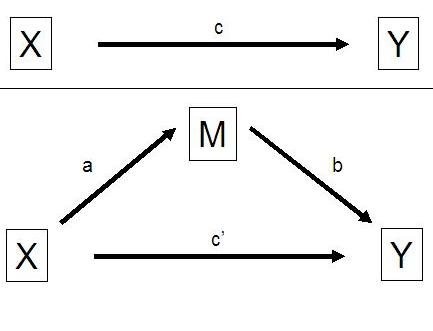
\includegraphics[scale = .5]{../images/mediation_image.jpg}
    \caption{Mediation Analysis: direct and indirect effects}
    \label{fig:mediationAnalysis}
  \end{center}
\end{figure}

Mediation analysis works by testing the extent to which the variance in the outcome attributable to a predictor variable (the direct effect, or path ``c'': $Y_i \sim d_Y + cX_i + e_i$) can be explained \textit{indirectly} by the variance of two other relationships: that of the predictor variable and a third mediator (X $\rightarrow$ M, or path ``a")  and M and the outcome variable (path ``b''), controlling for the direct relationship between X and Y (path ``'c'') (see Figure ~\ref{fig:mediationAnalysis}). The mediation model can thus be denoted by two equations:

\begin{equation}
  M_i \sim d_M + aX_i + e_Mi
\end{equation}

\begin{equation}
  Y_i \sim d_Y + bM_i + c'X_i +  + e_{Yi}
\end{equation}
\bigskip

When combined, these two equations enable the calculation of the ``indirect effect'' of the predictor on the outcome, by controlling for the relationship between the mediator's effect on the outcome variable as a function of its relationship to the predictor variable.  While the direct effect measures the extent to which the dependent variable changes when the independent variable increases by one unit and the mediator variable remains unaltered, the indirect effect measures the extent to which the dependent variable changes when the independent variable is held fixed and the mediator variable changes by the amount it would have changed had the independent variable increased by one unit \citep{Bauer2006}.

The multilevel structure of the data in this study, i.e. the clustering of residuals according to team affiliation, violates the independence assumption of mediation analysis. As such, traditional multiple linear regression and path analysis will produce biased tests of the effects in the mediation model \citep{Raudenbush2002}.
%(Hox, 2002; Kreft & de Leeuw, 1998; Raudenbush & Bryk, 2002).
A multilevel mediation analysis must therefore additionally take into account variance attributable to the random effects of the model (team, in this case), and in so doing capture heterogeneity of variance in the indirect effect due to the level 2 variable \citep{Tofighi2014}.  To do this, each coefficient in the model must be random (denoted by subscript ``j''), so that the value of the coefficient varies across Level 2 units (team): \\

\begin{equation}
  M_{ij} \sim d_{Mj} + a_jX_{ij} + e_{Mij}
\end{equation}

\begin{equation}
  Y_{ij} \sim d_{Yj} + b_jM_{ij} + 'c_jX_{ij} +  + e_{Yij}
\end{equation}
\bigskip

Linear mixed effects regression models are fitted according to these equations, and estimates of mediation effects can be computed from these model parameters.  Subsequent mediation analyses were conducted using the mediation() function of the Causal Mediation Analysis Package (version 4.4.5) in R.

\subsubsection{Roadmap of post-Tournament Analysis}
Analysis of the post-Tournament data proceeded by testing predictions associated with the overarching hypothesis, that higher perceptions of joint-action success would lead to higher levels of social bonding, mediated by feelings of ``team click''.

The first step was to assess whether the two variables hypothesised to be relevant to perceived joint-action success, 1) perceptions of component team performance (Joint Action Success) and 2) appraisal of team performance relative to prior expectations (Team Performance Expectations), predicted feelings of team click (Team Click). Controlling for athlete perceptions of individual performance success, subjective and objective technical competence, Tournament performance measures, and variation attributable to team membership (random effect), linear mixed-effect regression models were used to test the following predictions:

\begin{description}
  \item [Prediction 1.a] Joint Action Success  $\rightarrow$ Team Click
  \item [Prediction 1.b] Team Performance Expectations $\rightarrow$ Team Click
  \item [Prediction 1.c] Joint Action Success $\rightarrow$ Team Click, moderated by Team Performance Expectations
\end{description}

Next, the relationship between team click (Team Click) and social bonding (Social Bonding) was tested, controlling for subjective and objective technical competence, Tournament performance measures, and variation attributable to team membership (random effect):

\begin{description}
  \item [Prediction 2.a] Team Click $\rightarrow$ Social Bonding
\end{description}

Following this, the direct relationships between two predictor variables of interest (Joint Action Success and Team Performance Expectations) and social bonding was tested:

\begin{description}
  \item [Prediction 3.a] Joint Action Success $\rightarrow$ Social Bonding
  \item [Prediction 3.b] Team Performance Expectations $\rightarrow$ Social Bonding
\end{description}

Finally, a mediation analysis was performed to formally test whether feelings of team click mediated a direct relationship between perceptions of joint-action success and social bonding.

\begin{description}
\item[Prediction 4.a Mediation Analysis] Joint Action Success $\rightarrow$ Team Click $\rightarrow$ Social Bonding
\end{description}







\clearpage
\subsection{Analysis of pre-post Tournament data}
The predictions of the present study were further tested through an analysis of change in variables of interest between the pre- and post-Tournament surveys. By analysing pre-post Tournament responses, it was possible to investigate 1) to what extent variables of interest changed as a result of the Tournament, and 2) whether pre-post changes in variables of interest were consistent with study predictions concerning the relationship between joint-action and social bonding. When controlling for objective measures of success and feelings concerning individual performance, could change in social bonding be explained by changes in perceptions of joint-action success and/or changes in feelings of team click?


\subsubsection{Pre-post Tournament Descriptives}
Pre- and post-Tournament measures of variables of interest are displayed in tables below.  Three out of five variables designed to measure athletes' perceived success in components of individual performance significantly dropped following the Tournament (see Table ~\ref{tab:indPerformancePrePostSummary}).  Paired samples t-tests revealed significant negative mean differences between pre- and post-Tournament measures of passing technique
($M = -7.48 (-13.17, -1.80)$, $t(98)= -2.61,, p = .01$), support play ($M = -7.32 (-12.18, -2.47)$, $t(98)= -2.99,, p = .003$), and decision making in attack ($M = -5.19 ( -9.73, -0.65)$, $t(98)= -2.27,, p = .03$), while individual defence ($M = -3.42 (-9.01, 2.16)$, $t(98)= -1.22,, p = .23$), and effectiveness in contact ($M = -4.51 (-10.25, 1.24)$, $t(98)= -1.56,, p = .12$) did not decrease significantly between pre- and post-Tournament measures.  By contrast, all four variables designed to measure team success in components of joint-action did not differ significantly between pre- and post-Tournament measurements (see Table ~\ref{tab:teamPerformancePrePostSummary} for results).  Similarly, variables designed to measure team click also did not vary significantly.  These results suggest that athlelte perceptions of team joint-action success and team click on average remained stable throughout the Tournament.  Perceptions of success in individual component performance, by contrast, decreased significantly, indicating that following the Tournament athletes were on average more critical of their performance following the Tournament.\\

In terms of Social Bonding, both feelings of emotional support and feelings of shared goal with the team differed significantly between pre- and post-Tournament measurements (see Table ~\ref{tab:bondingPrePostSummary}). Both measures increased significantly in the post-Tournament measure (emotional support: $M = 9.30 (4.16, 14.45)$, $t(98)= 3.59,, p = .0005$; shared goal $M = 7.12 (3.06, 11.19)$, $t(98)= 3.48,, p = .0007$).  All other variables did not vary significantly from pre-Tournament measures, except for the pictorial measure of fusion to \textit{family}, which increased significantly, $M = .33 (0.03, 0.64)$, $t(98)= 2.18, p = .03$.  Bonding variables for which measures were 5-point Likert may have suffered from ceiling effects: the mean and median of each Fusion Pictorial scale was $> 4$.  In general, it appeared that bonding to the team (and to one measure of Family) increased when measured following the Tournament.

In addition, variables designed to measure feelings of fatigue also varied significantly between pre- and post-Tournament measurements.  Fatigue ($M = 21.61 (15.02 28.20)$, $t(116)= 6.49,, p < .0001$), physical perceived exertion ($M = 2.84 (1.89, 3.79)$, $t(116)= 5.93, p < .0001$), and mental perceived exertion ($M = 2.84 (1.89, 3.79)$, $t(116)= 5.93, p < .0001$) all increased significantly from the point of first measurement immediately llowing the 2nd game on day 1 of the Tournament (see Table ~\ref{tab:fatiguePrePostSummary}).  Injury status did not differ significantly from pre-Tournament measures, although the mean difference did appear to increase, $M = 2.84 (-10.63, 0.59)$, $t(98)= 1.78, p = .08$.  These results indicate that on average, athletes felt higher levels of exertion and fatigue after the Tournament, than they did before or after the first game of the Tournament. This is to be expected, given the intensity of the rugby sevens Tournament format. It provides confirmation for the strenuous nature of the activity of the present study.


\newgeometry{margin=0.5cm} % modify this if you need even more space
\begin{landscape}

% Table created by stargazer v.5.2 by Marek Hlavac, Harvard University. E-mail: hlavac at fas.harvard.edu
% Date and time: Sun, Jun 25, 2017 - 22:44:09
\begin{table}[!htbp] \centering 
  \caption{Individual Performance change pre-post Tournament} 
  \label{tab:indPerformancePrePostSummary} 
\footnotesize 
\begin{tabular}{@{\extracolsep{5pt}} cccccccccc} 
\\[-1.8ex]\hline 
\hline \\[-1.8ex] 
 & Variable & Mean.pre & SD.pre & Mean.post & SD.post & MeanDiffernece & MeanPairedDifference & t-test & p-value \\ 
\hline \\[-1.8ex] 
1 & passingTechnique & $65.74$ & $24.94$ & $58.41$ & $24.25$ & $$-$7.33$ & $$-$7.48$ & $$-$2.61$ & $0.01$ \\ 
2 & supportPlay & $69.54$ & $23.23$ & $62.62$ & $22.70$ & $$-$6.92$ & $$-$7.32$ & $$-$2.99$ & $0.003$ \\ 
3 & individualDefense & $59.22$ & $26.64$ & $57.64$ & $23.57$ & $$-$1.57$ & $$-$3.42$ & $$-$1.22$ & $0.23$ \\ 
4 & effectivenessContact & $65.66$ & $24.85$ & $62.15$ & $24.81$ & $$-$3.51$ & $$-$4.51$ & $$-$1.56$ & $0.12$ \\ 
5 & decisionMakingAttack & $65.48$ & $23.80$ & $61.22$ & $21.43$ & $$-$4.26$ & $$-$5.19$ & $$-$2.27$ & $0.03$ \\ 
\hline \\[-1.8ex] 
\end{tabular} 
\end{table} 


% Table created by stargazer v.5.2 by Marek Hlavac, Harvard University. E-mail: hlavac at fas.harvard.edu
% Date and time: Sun, Jun 25, 2017 - 22:47:06
\begin{table}[!htbp] \centering 
  \caption{Team Performance change pre-post Tournament} 
  \label{tab:teamPerformancePrePostSummary} 
\footnotesize 
\begin{tabular}{@{\extracolsep{5pt}} cccccccccc} 
\\[-1.8ex]\hline 
\hline \\[-1.8ex] 
 & Variable & Mean.pre & SD.pre & Mean.post & SD.post & MeanDiffernece & MeanPairedDifference & t-test & p-value \\ 
\hline \\[-1.8ex] 
1 & teamDefense & $65.06$ & $22.85$ & $62.42$ & $22.50$ & $$-$2.63$ & $$-$4.92$ & $$-$1.57$ & $0.12$ \\ 
2 & teamAttack & $66.01$ & $24.95$ & $65.33$ & $20.26$ & $$-$0.68$ & $$-$1.59$ & $$-$0.55$ & $0.58$ \\ 
3 & teamSupportPlay & $64.36$ & $23.53$ & $65.75$ & $19.72$ & $1.40$ & $0.90$ & $0.35$ & $0.73$ \\ 
4 & teamCommunication & $62.37$ & $24.21$ & $65.25$ & $21.26$ & $2.89$ & $$-$0.07$ & $$-$0.03$ & $0.98$ \\ 
\hline \\[-1.8ex] 
\end{tabular} 
\end{table} 


% Table created by stargazer v.5.2 by Marek Hlavac, Harvard University. E-mail: hlavac at fas.harvard.edu
% Date and time: Sat, Jun 03, 2017 - 15:44:29
\begin{table}[!htbp] \centering 
  \caption{click change pre-post Tournament} 
  \label{} 
\footnotesize 
\begin{tabular}{@{\extracolsep{5pt}} cccccccccc} 
\\[-1.8ex]\hline 
\hline \\[-1.8ex] 
 & Variable & Mean.pre & SD.pre & Mean.post & SD.post & MeanDiffernece & MeanPairedDifference & t-test & p-value \\ 
\hline \\[-1.8ex] 
1 & unspokenUnderstanding & $71.58$ & $20.77$ & $72.72$ & $19.95$ & $1.14$ & $1.33$ & $0.58$ & $0.56$ \\ 
2 & generalAtmosphere & $75.51$ & $23.27$ & $78.45$ & $21.34$ & $2.94$ & $1.05$ & $0.47$ & $0.64$ \\ 
3 & clickPictorial & $3.87$ & $1.24$ & $3.93$ & $1.04$ & $0.07$ & $0.03$ & $0.21$ & $0.84$ \\ 
4 & reliabilityOfOthers & $67.43$ & $28.01$ & $68$ & $23.09$ & $0.57$ & $1.21$ & $0.40$ & $0.69$ \\ 
5 & reliabilityForOthers & $62.38$ & $25.40$ & $63.45$ & $25.80$ & $1.07$ & $1.06$ & $0.38$ & $0.70$ \\ 
6 & abilityExtended & $70.45$ & $25.83$ & $72.25$ & $19.27$ & $1.80$ & $1.43$ & $0.53$ & $0.60$ \\ 
\hline \\[-1.8ex] 
\end{tabular} 
\end{table} 


% Table created by stargazer v.5.2 by Marek Hlavac, Harvard University. E-mail: hlavac at fas.harvard.edu
% Date and time: Sun, Jun 25, 2017 - 22:51:01
\begin{table}[!htbp] \centering 
  \caption{bonding change pre-post Tournament} 
  \label{tab:bondingPrePostSummary} 
\footnotesize 
\begin{tabular}{@{\extracolsep{5pt}} cccccccccc} 
\\[-1.8ex]\hline 
\hline \\[-1.8ex] 
 & Variable & Mean.pre & SD.pre & Mean.post & SD.post & MeanDiffernece & MeanPairedDifference & t-test & p-value \\ 
\hline \\[-1.8ex] 
1 & emotionalSupport & $70.12$ & $26.21$ & $79.67$ & $18.84$ & $9.55$ & $9.30$ & $3.59$ & $0.001$ \\ 
2 & sharedGoal & $77.66$ & $24.28$ & $86$ & $15.56$ & $8.34$ & $7.12$ & $3.48$ & $0.001$ \\ 
3 & groupId & $4.34$ & $0.78$ & $4.29$ & $0.67$ & $$-$0.04$ & $0.06$ & $0.78$ & $0.44$ \\ 
4 & fusionVerbal & $4.03$ & $0.74$ & $4.00$ & $0.71$ & $$-$0.03$ & $0$ & $0$ & $1$ \\ 
5 & fusionPictorialTeam & $4.26$ & $1.25$ & $4.33$ & $1.19$ & $0.07$ & $0.04$ & $0.30$ & $0.77$ \\ 
6 & fusionPictorialCountry & $4.01$ & $1.58$ & $4.03$ & $1.39$ & $0.02$ & $$-$0.04$ & $$-$0.22$ & $0.83$ \\ 
7 & fusionPictorialFamily & $4.10$ & $1.50$ & $4.51$ & $0.96$ & $0.41$ & $0.33$ & $2.18$ & $0.03$ \\ 
8 & rankTeam & $1.49$ & $0.79$ & $1.61$ & $0.81$ & $0.12$ & $0.09$ & $1.15$ & $0.25$ \\ 
9 & rankCountry & $1.92$ & $1.06$ & $1.93$ & $1.03$ & $$ & $$-$0.04$ & $$-$0.44$ & $0.66$ \\ 
10 & rankFamily & $1.41$ & $0.88$ & $1.42$ & $0.86$ & $0.01$ & $0$ & $0$ & $1$ \\ 
\hline \\[-1.8ex] 
\end{tabular} 
\end{table} 


% Table created by stargazer v.5.2 by Marek Hlavac, Harvard University. E-mail: hlavac at fas.harvard.edu
% Date and time: Sun, Jun 25, 2017 - 23:08:36
\begin{table}[!htbp] \centering 
  \caption{Fatigue change pre-post Tournament} 
  \label{fatiguePrePostSummary} 
\footnotesize 
\begin{tabular}{@{\extracolsep{5pt}} cccccccccc} 
\\[-1.8ex]\hline 
\hline \\[-1.8ex] 
 & Variable & Mean.pre & SD.pre & Mean.post & SD.post & MeanDiffernece & MeanPairedDifference & t-test & p-value \\ 
\hline \\[-1.8ex] 
1 & fatigue & $50.14$ & $28.80$ & $69.27$ & $21.24$ & $19.13$ & $21.61$ & $6.49$ & $0$ \\ 
2 & prpe & $12.45$ & $4.52$ & $14.97$ & $2.66$ & $2.52$ & $2.84$ & $5.93$ & $0.0000$ \\ 
3 & mental & $4.09$ & $2.83$ & $6.08$ & $2.47$ & $1.99$ & $2.30$ & $6.85$ & $0$ \\ 
4 & injury & $81.28$ & $23.36$ & $76.14$ & $26.91$ & $$-$5.13$ & $5.02$ & $1.78$ & $0.08$ \\ 
\hline \\[-1.8ex] 
\end{tabular} 
\end{table} 


% Table created by stargazer v.5.2 by Marek Hlavac, Harvard University. E-mail: hlavac at fas.harvard.edu
% Date and time: Sat, Jun 03, 2017 - 17:41:41
\begin{table}[!htbp] \centering 
  \caption{factors change pre-post Tournament} 
  \label{} 
\footnotesize 
\begin{tabular}{@{\extracolsep{5pt}} cccccccccc} 
\\[-1.8ex]\hline 
\hline \\[-1.8ex] 
 & Variable & Mean.pre & SD.pre & Mean.post & SD.post & MeanDiffernece & MeanPairedDifference & t-test & p-value \\ 
\hline \\[-1.8ex] 
1 & teamPerformanceFactorPrePost & $$-$0.01$ & $1.04$ & $0.01$ & $0.88$ & $0.01$ & $$-$0.06$ & $$-$0.48$ & $0.63$ \\ 
2 & indPerformanceFactorPrePost & $0.12$ & $0.95$ & $$-$0.13$ & $0.93$ & $$-$0.25$ & $$-$0.28$ & $$-$2.99$ & $0.004$ \\ 
3 & clickFactorPrePost & $$-$0.04$ & $0.98$ & $0.04$ & $0.85$ & $0.09$ & $0.06$ & $0.69$ & $0.84$ \\ 
4 & bondingFactorPrePost & $$-$0.18$ & $1.03$ & $0.19$ & $0.71$ & $0.37$ & $0.34$ & $3.74$ & $0.0003$ \\ 
5 & fatigueFactorPrePost & $$-$0.29$ & $1.01$ & $0.40$ & $0.65$ & $0.68$ & $0.77$ & $7.03$ & $0$ \\ 
\hline \\[-1.8ex] 
\end{tabular} 
\end{table} 

\end{landscape}
\restoregeometry



\subsubsection{Data Reduction}
As in the analysis of the pre- and post-Tournament survey responses, data reduction was performed in order to consolidate measures of interest into underlying factors. The following results are extracted from EFAs using an oblique rotation method in R (see details above).

\myparagraph{Component Performance}
Four survey items related to perceptions of component performance (team and individual) were collected and subjected to factor analysis. For items relating to components of team performance, one factor was imposed (labelled ``Joint Action Success Pre Post''),  which explained 74.5\% of the overall variance (SS Loading = 2.97).  Various statistics, including $KMO = 0.82$, corrtest Bartlett: $\chi^2(6, N = 238) = 717.55$, $p < .001$ and $Guttman's \lambda =.90$ and $Cronbach's \alpha = (.92)$ indicated that the data reduction was appropriate. Five items relating to components of individual performance were subjected to EFA. One factor—``Ind Performance Success Pre Post''—was imposed, which explained 59.9\% of the overall variance (SS Loading = 2.99).  Various statistics, including $KMO = 0.83$, corrtest Bartlett: $\chi^2(10, N = 238) = 633.82$, $p < .001$ and $Guttman's\lambda =.87$ and $Cronbach's \alpha = .88$ indicated that the data reduction was appropriate.
%$\chi^2 (df=2) = 20.27$, $p < .001$,
%$\chi^2 (df=5) = 47.29$, $p < .001$,

\myparagraph{Team Click}
Six survey items related to feelings of team click (``Team Click Pre Post'') were collected and subjected to EFA. One factor was imposed, $\chi^2(9, N = 238) = 31.52 $, $p < .001$, which explained 37.6\% of the overall variance (SS Loading = 2.26).  Various statistics, including $KMO = 0.78$, corrtest Bartlett: $\chi^2(15, N = 238) = 336.41$, $p < .001$ and $Guttman's \lambda =.76$ and $Cronbach's \alpha = .76$ indicated that the data reduction was appropriate.

\myparagraph{Social Bonding}
Four survey items related to feelings of social bonding were subjected to EFA. One factor, labelled ``Social Bonding Pre Post'' was extracted, which explained 41.9\% of the overall variance (SS Loading = 1.68).  Various statistics, including $KMO = 0.66$, corrtest Bartlett: $\chi^2(6, N = 238) = 218.95$, $p < .001$ and $Guttman's \lambda =.68$ and $Cronbach's \alpha = .71$ indicated that the data reduction was appropriate.
% $\chi^2 (df=2) = 10.3 $, $p < .01$,

\myparagraph{Fatigue}
Three survey items related to feelings of fatigue (``Fatigue Pre Post'') were collected and subjected to EFA. One factor was imposed, $\chi^2(0, N = 238) = 0 $, $p < .001$, which explained 66.3\% of the overall variance (SS Loading = 1.99).  $KMO = .7$, corrtest Bartlett: $\chi^2(3, N = 238) = 382.88$, $p < .001$ and $Guttman's \lambda =.8$ and $Cronbach's \alpha = .85$ indicated that the data reduction was appropriate.

\subsubsection{Pre-post differences in latent factors}
Following data reduction, paired samples t-tests were used to compare pre- and post-Tournament measures of extracted factors relating to team and individual performance, team click, social bonding, and fatigue. Results are displayed in Table ~\ref{}.  Mean difference between athlete scores of team component performance (Joint Action Success Pre Post) did not vary significantly from pre- to post-Tournament, $M = -.06 (-0.30  0.18)$, $t(98)= -.48, p = .63$, nor did team click, $M = .06 (-0.12, 0.25)$, $t(98)= .69, p = .49$. Athlete mean differences in perceptions of components of individual performance (Ind Performance Success Pre Post) significantly decreased following the Tournament, $M = -0.28 (-0.47, -0.10)$, $t(98)= -2.99, p = .003$, confirming that athletes were an average more critical of their individual performance at the completion of the Tournament.

Tests revealed that the there was a significant difference in athlete reports of social bonding between pre- and post-Tournament measurements, $M = 0.34 (0.16, 0.52)$, $t(98)= 3.73, p = .0003$, Athletes' feelings of bonding on average increased after the Tournament.  Average ratings of fatigue also significantly increased from measurement following athletes' second game on day 1  to ratings following the Tournament, $M =  0.77 (0.55, 0.99)$, $t(116)= 7.03, p < .0001$.
\clearpage




\subsection{Model Selection}
The summary statistics outline above suggested that further analysis into the relationships between changing variables was appropriate. The number of observations available in the pre-post Tournament data were insufficient to construct a mixed-effects repeated measures design in which both the intercept and slope of observations could vary according to each individual athlete nested within their given team over time.\footnote{Allowing both the intercept and slope to vary requires twice the number of observations to estimate the random effects ($2x174 = 248$), whereas the available number of observations was only 198} Alternative models for suitable for repeated measures designs, such as RM-ANOVA or ANCOVA, are also incapable of allowing each fixed factor (the regression coefficient or slope) to vary randomly according to higher level factors (individual and team), and are also unable to handle unbalanced designs (in this case, due missing data for athletes across pre- and post-Tournament measurements). As a compromise, change scores in variables of interest (individual and team performance, team click, social bonding, and fatigue) were calculated by subtracting pre- from post-Tournament scores for each athlete. The calculation of change scores reduced the complexity of the data structure to only two levels of analysis, and meant that relationships between these change variables could be modelled using a linear mixed effects regression. Change scores of relevant factors were introduced to the model as fixed effects, and their slopes and intercepts were allowed to vary according to team.





\subsubsection{Roadmap of pre-post Tournament Analysis}
Analysis of the pre-post Tournament data proceeded in the same manner as the post-Tournament data. The hypothesised relationship between joint-action success and social bonding was broken down into component relationships. \\

First, changes in feelings of team click were analysed as a function of changes in 1) perceptions of team component performance (Joint Action Success Pre Post), 2) post-Tournament appraisal of team performance relative to prior expectations (Team Performance Expectations), and 3) the interaction between these two predictor variables.
\bigskip
\begin{description}
  \item [Prediction 2.1.a] $\Delta$Joint Action Success  $\rightarrow$  $\Delta$Team Click
  \item [Prediction 2.1.b] $\Delta$Team Performance Expectations $\rightarrow$ $\Delta$ Team Click
  \item [Prediction 2.1.c] $\Delta$Joint Action Success $\rightarrow$ $\Delta$Team Click, moderated by $\Delta$Team Performance Expectations
\end{description}

Second, the change observed in social bonding (Social Bonding Pre Post) was analysed as a function of change in feelings of team click.
\bigskip
\begin{description}
  \item [Prediction 2.2.a] $\Delta$Team Click $\rightarrow$ $\Delta$Social Bonding
\end{description}

Third, the direct relationships between predictor variables (change in perceptions of join-action success and appraisal of team performance relative to prior expectation) and change in social bonding was analysed:
\bigskip
\begin{description}
  \item [Prediction 2.3.a] $\Delta$Joint Action Success $\rightarrow$ $\Delta$Social Bonding
  \item [Prediction 2.3.b] $\Delta$Team Performance Expectations $\rightarrow$ $\Delta$Social Bonding
\end{description}

Finally, a mediation analysis was performed to formally test whether feelings of team click mediated a direct relationship between perceptions of joint-action success and social bonding.

\begin{description}
  \item[Prediction 2.4.a Mediation Analysis] $\Delta$Joint Action Success $\rightarrow$ $\Delta$Team Click $\rightarrow$ $\Delta$Social Bonding
\end{description}



\clearpage














\subsection{Analysis of overall Tournament data}

In the final section of analysis, evidence for a relationship between joint-action success, team click, and social bonding was assessed across the entire data set. Given that the mid-Tournament survey was truncated to accord with athlete schedules and convenience following games, variables that could be analysed across the entire tournament were limited to those that appeared in the mid-Tournament surveys. Time constraints meant that component performance was not assessed in the mid-Tournament survey, and only appraisals of overall individual and team performance relative to prior expectations were included. The mid-Tournament survey contained three team click items (Unspoken Understanding, General Atmosphere, and Click Pictorial), three social bonding items (Emotional Support, Shared Goal, and Fusion Pictorial), and three fatigue items (Fatigue, Physical Exertion, Mental Exertion). These groups of variables were all subjected to data reduction (EFA).

\subsubsection{Descriptive Statistics: ``Toys out of the Pram''}

Tables~\ref{tab:performanceOverallSummary}\nobreakdash--\ref{tab:fatigueOverallSummary} display basic summary statistics (mean and standard deviation) for variables of interest at each recorded time point. Almost all variables of interest under the categories of performance, team click, social bonding and fatigue have means above the mid-point of each scale. In addition, mid-Tournament measurements tend to be lower than pre- or post-Tournament measures for each category. In relation to performance measures, for example, athletes appear on average to be more critical of their own and their team’s performance (relative to prior expectations) when surveyed immediately after games on day 1 and 2 than they were following the Tournament (note that survey items relating to individual and team performance administered pre-Tournament were not posed in relation to athlete expectations, and thus could not be directly compared to subsequent mid- and post-Tournament measures). The same pattern was identifiable in team click variables, with the means for mid-Tournament measures of Unspoken Understanding and General Atmosphere 10-15\% lower than pre- or post-Tournament measures. This is also the case for variables related to social bonding: Emotional Support and Shared Goal in particular showing a steep increase form mid-Tournament measurements to the post-Tournament measurement. The same pattern was identifiable for variables relevant to fatigue (see Table ~\ref{tab:fatigueOverallSummary}).\\


% Table created by stargazer v.5.2 by Marek Hlavac, Harvard University. E-mail: hlavac at fas.harvard.edu
% Date and time: Mon, Jun 26, 2017 - 09:48:21
\begin{table}[!htbp] \centering 
  \caption{Overall Tournament Performance Summary Statistics} 
  \label{tab:performanceOverallSummary} 
\scriptsize 
\begin{tabular}{@{\extracolsep{5pt}} ccccccccc} 
\\[-1.8ex]\hline 
\hline \\[-1.8ex] 
time & teamPerf & tP.sd & indPerf & iP.sd & teamPerfExp & tPE.sd & indPerfExp & iP.sd.1 \\ 
\hline \\[-1.8ex] 
pre-Tournament & $71.11$ & $21.87$ & $68.92$ & $21.32$ & $$ & $$ & $$ & $$ \\ 
day1 & $$ & $$ & $$ & $$ & $54.43$ & $30.63$ & $39.43$ & $27.25$ \\ 
day2 & $$ & $$ & $$ & $$ & $53.19$ & $32.98$ & $40.92$ & $27.93$ \\ 
post-Tournament & $$ & $$ & $$ & $$ & $64.36$ & $23.61$ & $56.36$ & $23.47$ \\ 
\hline \\[-1.8ex] 
\end{tabular} 
\end{table} 


% Table created by stargazer v.5.2 by Marek Hlavac, Harvard University. E-mail: hlavac at fas.harvard.edu
% Date and time: Mon, Jun 26, 2017 - 09:21:29
\begin{table}[!htbp] \centering 
  \caption{Team Click Overall Tournament Summary Statistics} 
  \label{tab:clickOverallSummary} 
\scriptsize 
\begin{tabular}{@{\extracolsep{5pt}} ccccccc} 
\\[-1.8ex]\hline 
\hline \\[-1.8ex] 
time & unspUnd & uU.sd & genAt & gA.sd & clickPic & cP.sd \\ 
\hline \\[-1.8ex] 
pre-Tournament & $71.58$ & $20.77$ & $75.51$ & $23.27$ & $3.87$ & $1.24$ \\ 
day1 & $55.92$ & $26.88$ & $65.74$ & $31.95$ & $3.46$ & $1.49$ \\ 
day2 & $55.30$ & $29.43$ & $64.32$ & $33.39$ & $3.33$ & $1.70$ \\ 
post-Tournament & $72.72$ & $19.95$ & $78.45$ & $21.34$ & $3.93$ & $1.04$ \\ 
\hline \\[-1.8ex] 
\end{tabular} 
\end{table} 


% Table created by stargazer v.5.2 by Marek Hlavac, Harvard University. E-mail: hlavac at fas.harvard.edu
% Date and time: Mon, Jun 26, 2017 - 09:22:14
\begin{table}[!htbp] \centering 
  \caption{Social Bonding Overall Tournament Summary Statistics} 
  \label{tab:bondingOverallSummary} 
\scriptsize 
\begin{tabular}{@{\extracolsep{5pt}} ccccccc} 
\\[-1.8ex]\hline 
\hline \\[-1.8ex] 
time & emoSup & eS.sd & sharedGoal & sG.sd & fusionPic & fP.sd \\ 
\hline \\[-1.8ex] 
pre-Tournament & $70.12$ & $26.21$ & $77.66$ & $24.28$ & $4.26$ & $1.25$ \\ 
day1 & $67.29$ & $30.56$ & $76.34$ & $30.50$ & $4.06$ & $1.47$ \\ 
day2 & $67.53$ & $32.55$ & $71.42$ & $35.47$ & $3.85$ & $1.69$ \\ 
post-Tournament & $79.67$ & $18.84$ & $86$ & $15.56$ & $4.33$ & $1.19$ \\ 
\hline \\[-1.8ex] 
\end{tabular} 
\end{table} 


% Table created by stargazer v.5.2 by Marek Hlavac, Harvard University. E-mail: hlavac at fas.harvard.edu
% Date and time: Mon, Jun 26, 2017 - 09:23:43
\begin{table}[!htbp] \centering 
  \caption{Fatigue Overall Tournament Summary Statistics} 
  \label{tab:fatigueOverallSummary} 
\scriptsize 
\begin{tabular}{@{\extracolsep{5pt}} ccccccccc} 
\\[-1.8ex]\hline 
\hline \\[-1.8ex] 
time & fat & f.sd & prpe & p.sd & mental & m.sd & inj.mu & inj.sd \\ 
\hline \\[-1.8ex] 
pre-Tournament & $$ & $$ & $$ & $$ & $$ & $$ & $18.73$ & $23.36$ \\ 
day1 & $50.14$ & $28.80$ & $12.45$ & $4.52$ & $4.09$ & $2.83$ & $29.91$ & $33.15$ \\ 
day2 & $53.65$ & $31.03$ & $12.60$ & $5.53$ & $4.13$ & $3.17$ & $37.14$ & $37.66$ \\ 
post-Tournament & $69.27$ & $21.24$ & $14.97$ & $2.66$ & $6.08$ & $2.47$ & $23.86$ & $26.91$ \\ 
\hline \\[-1.8ex] 
\end{tabular} 
\end{table} 


An examination of the frequency distributions for each variable reveals that lower mean scores for mid-Tournament measurements could be explained by high frequencies of extremely low values (zero or near zero) for performance, team-click, social bonding, and fatigue relative to pre- or post-Tournament measurement.  While pre- and post-Tournament distributions appear to be generally near-normal in terms of kurtosis (but with slight-to-moderate negative skew), almost all mid-Tournament distributions were clearly not-normally distributed, with some appearing almost bi-model due to the high frequency of zero or near-zero values (see time series frequency distributions for each variable, Figures ~\ref{fig:teamPerformanceDist}\nobreakdash--\ref{fig:mentalDist}).  In the case of individual and team performance relative to prior expectations, only 4 of 118 Individual Performance Expectations and 1 of 118 Team Performance Expectations post-Tournament observations were zero (indicating extremely poor performance relative to prior expectations), whereas the same questions on Day 1 of the Tournament received 30 of 164 (18\%) zero responses for Ind Performance Expectations and 22 of 164 (13\%) for Team Performance Expectations; Day 2 received 28 of 164 (17\%) zero responses for Ind Performance Expectations and 24 of 164 (15\%) for Team Performance Expectations.  While not directly comparable to the mid- and post-Tournament measures, the pre-Tournament measure of recent individual and team performance, ``Over the past month, how well do you feel you personally/your team have been performing overall in training and competition?'' only recorded totals of 4/120 (individual) and 5/120 (team) zero scores (see frequency distribution histograms in appendix).

This pattern of extremely low scores for mid-Tournament measures relative to pre- and mid-Tournament measures is consistent for team click, social bonding, and fatigue.

% teamPerformance
\begin{figure}[htbp]
  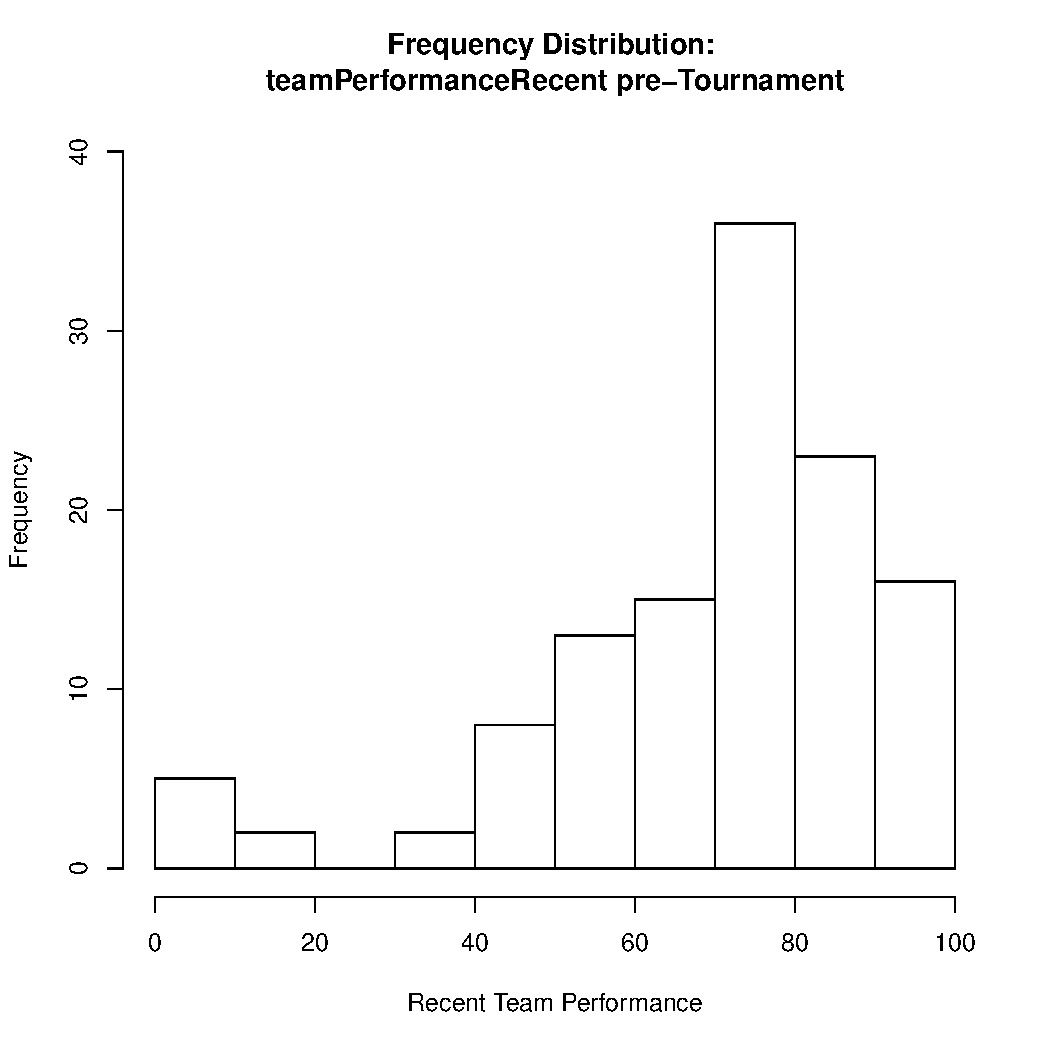
\includegraphics[scale =.4]{../images/distTeamPerformancePre.pdf}
  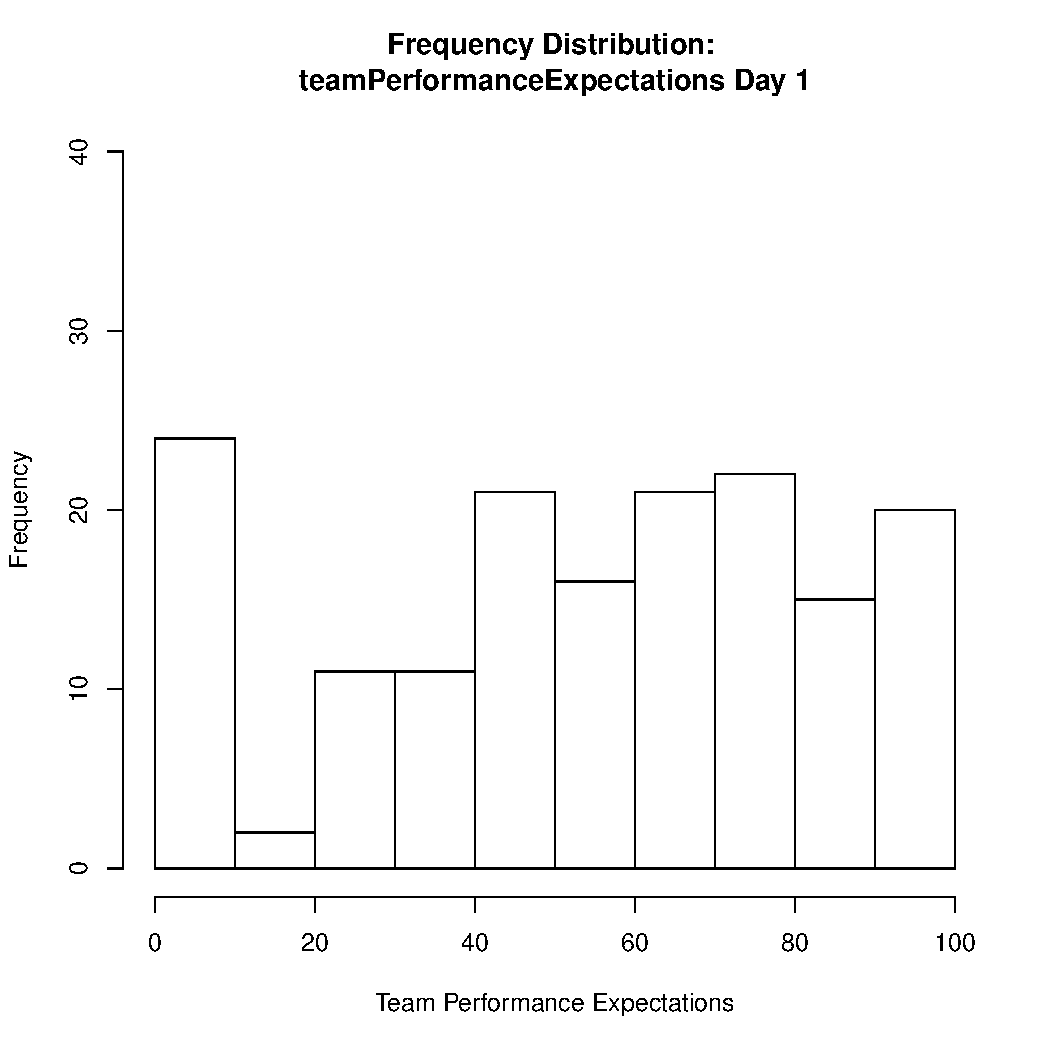
\includegraphics[scale =.4]{../images/distTeamPerfExpDay1.pdf}
  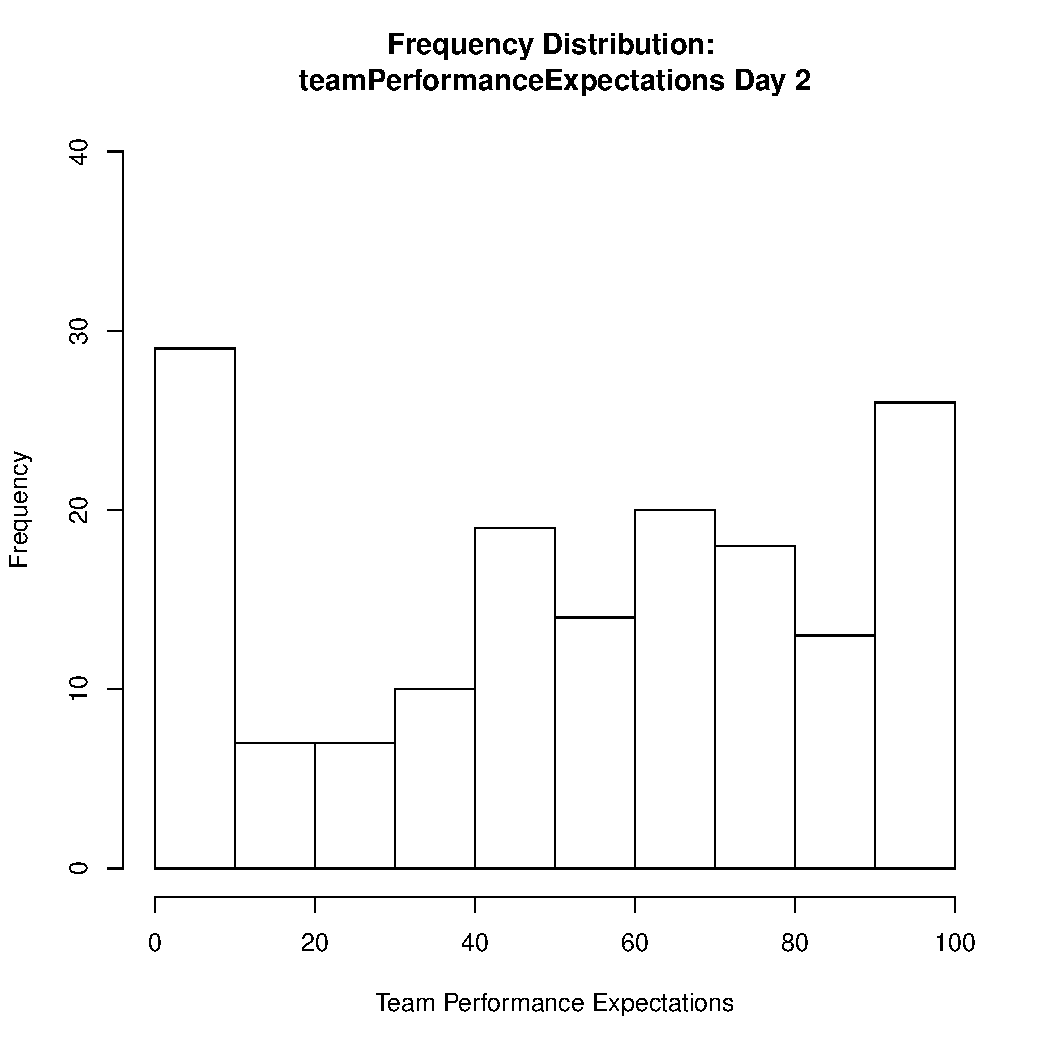
\includegraphics[scale =.4]{../images/distTeamPerfExpDay2.pdf}
  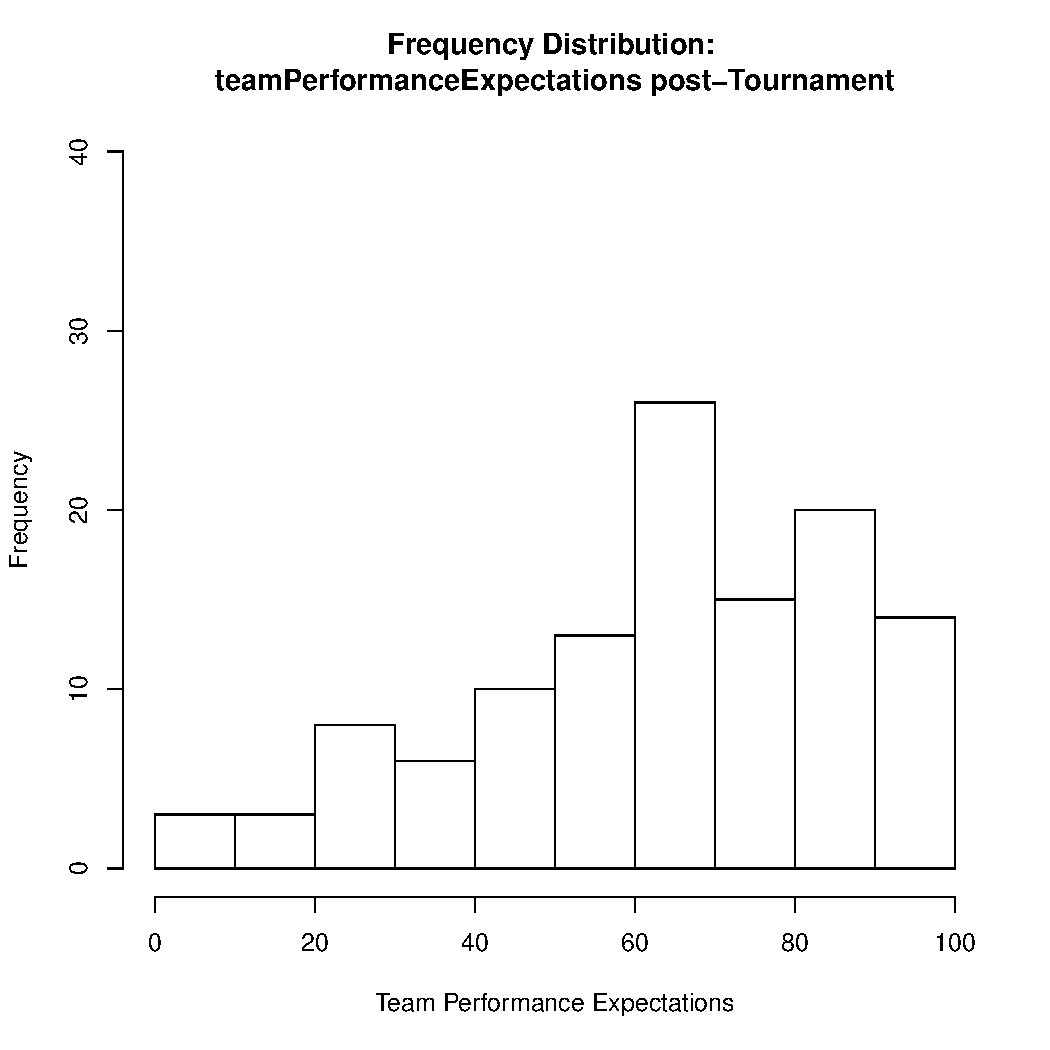
\includegraphics[scale =.4]{../images/distTeamPerfExpPost.pdf}
  \caption{Team Performance Frequency Distributions}
  \label{fig:teamPerformanceDist}
\end{figure}

%indPerformance
\begin{figure}[htbp]
  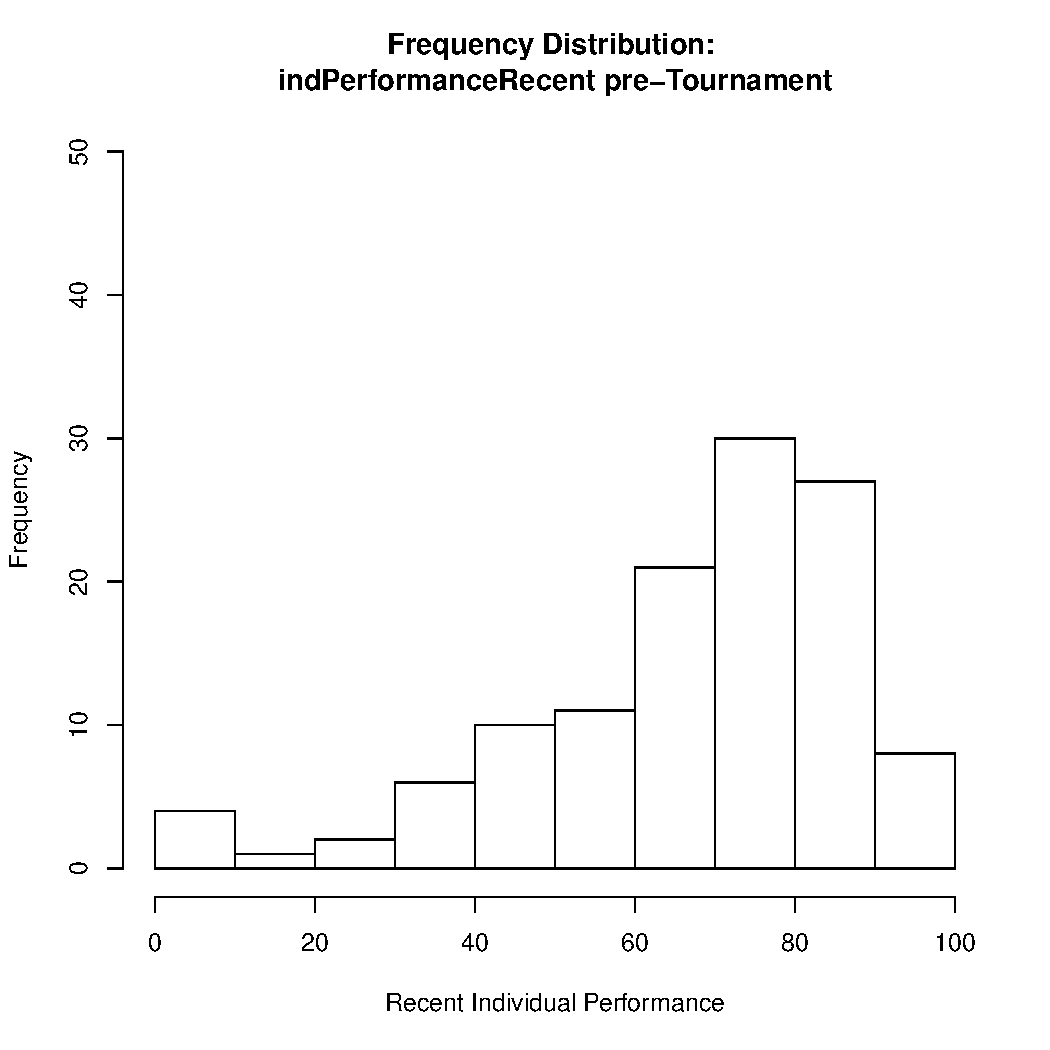
\includegraphics[scale =.4]{../images/distIndPerformancePre.pdf}
  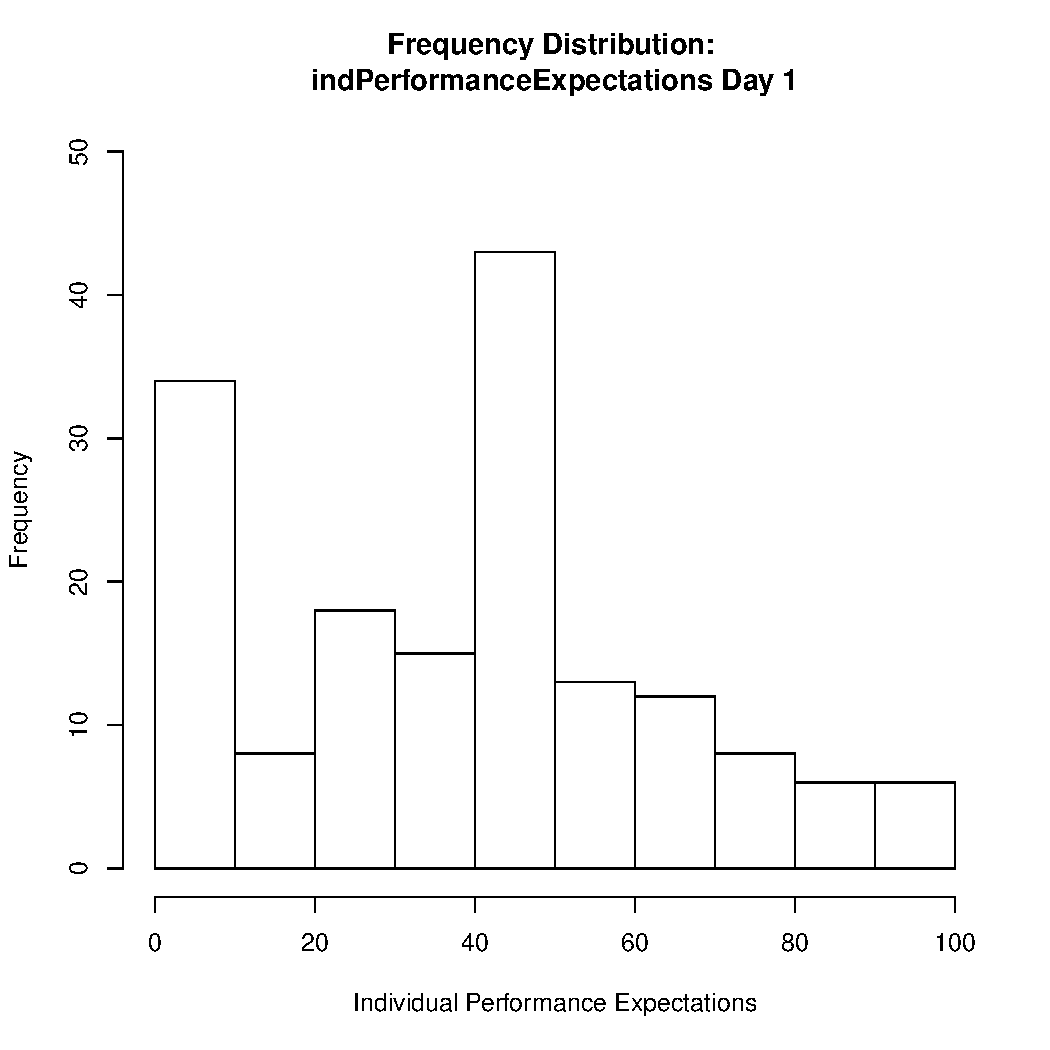
\includegraphics[scale =.4]{../images/distIndPerfExpDay1.pdf}
  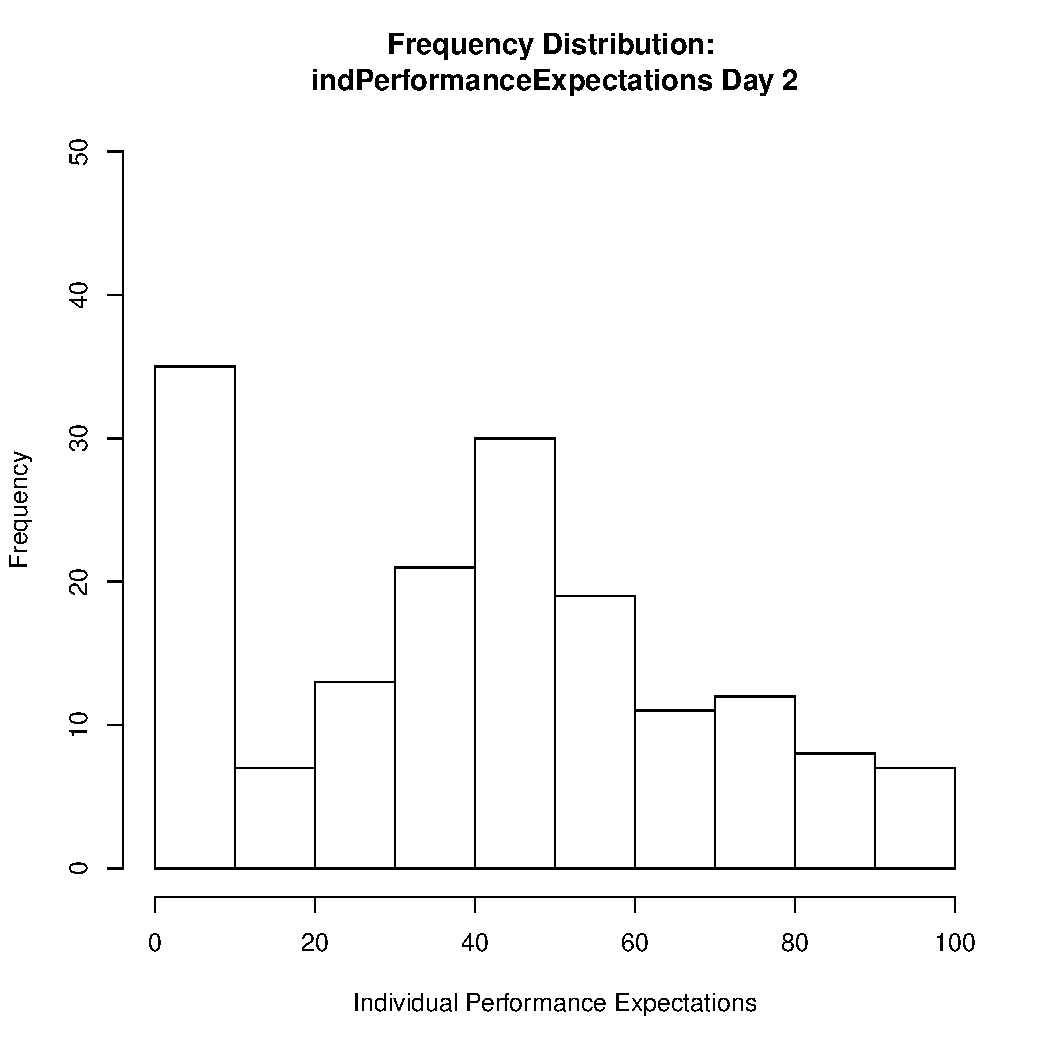
\includegraphics[scale =.4]{../images/distIndPerfExpDay2.pdf}
  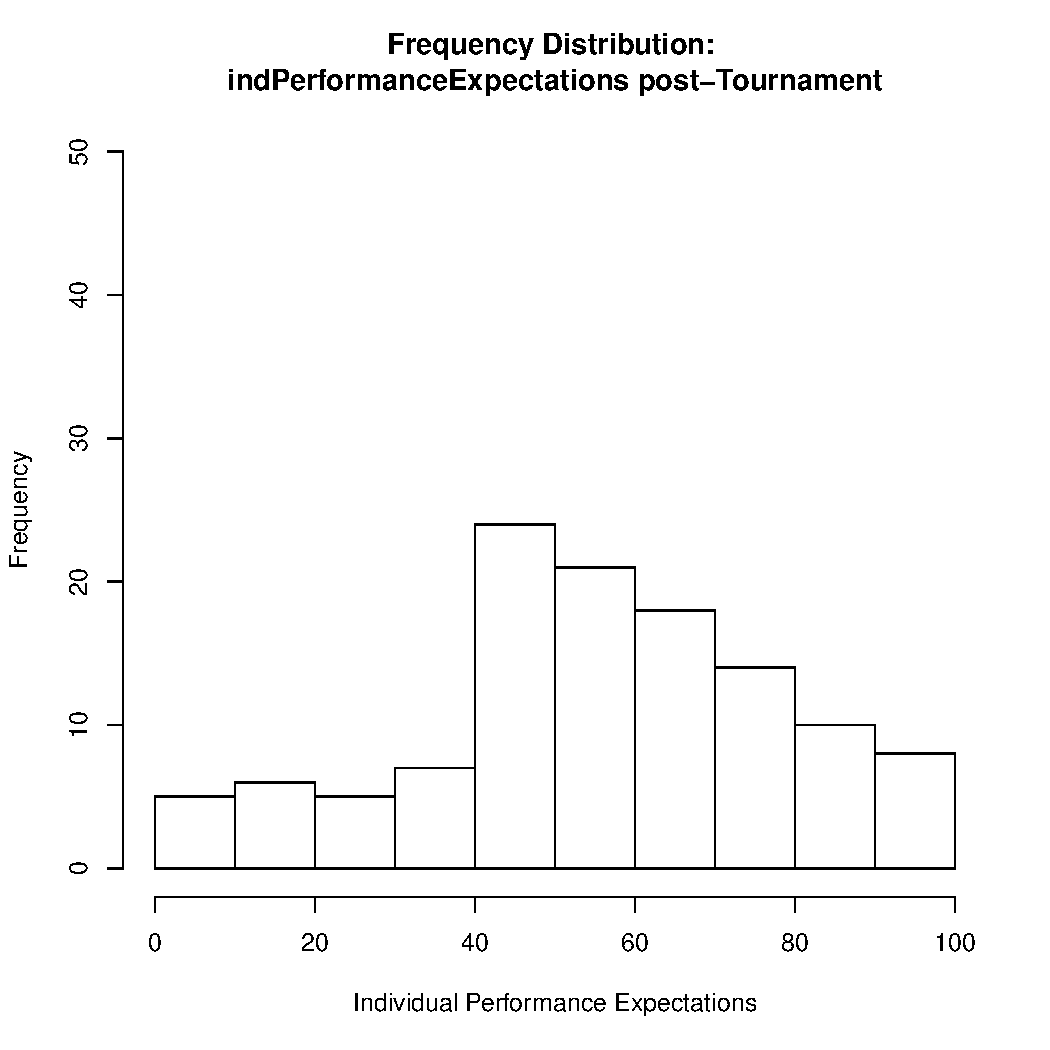
\includegraphics[scale =.4]{../images/distIndPerfExpPost.pdf}
  \caption{Individual Performance Frequency Distributions}
  \label{fig:indPerformanceDist}
\end{figure}
%click:
%unspokenUnderstanding
\begin{figure}[htbp]
  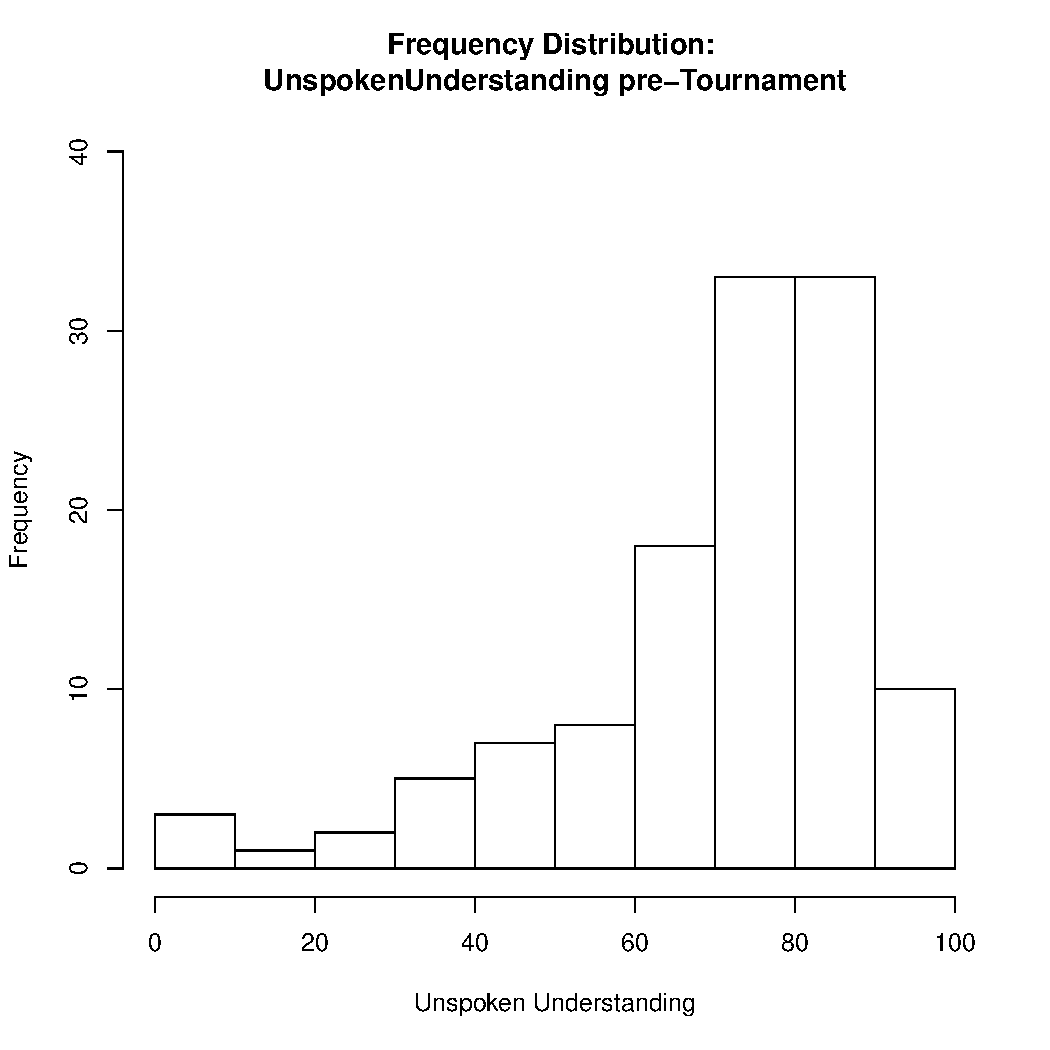
\includegraphics[scale =.4]{../images/distUnspokenUnderstandingPre.pdf}
  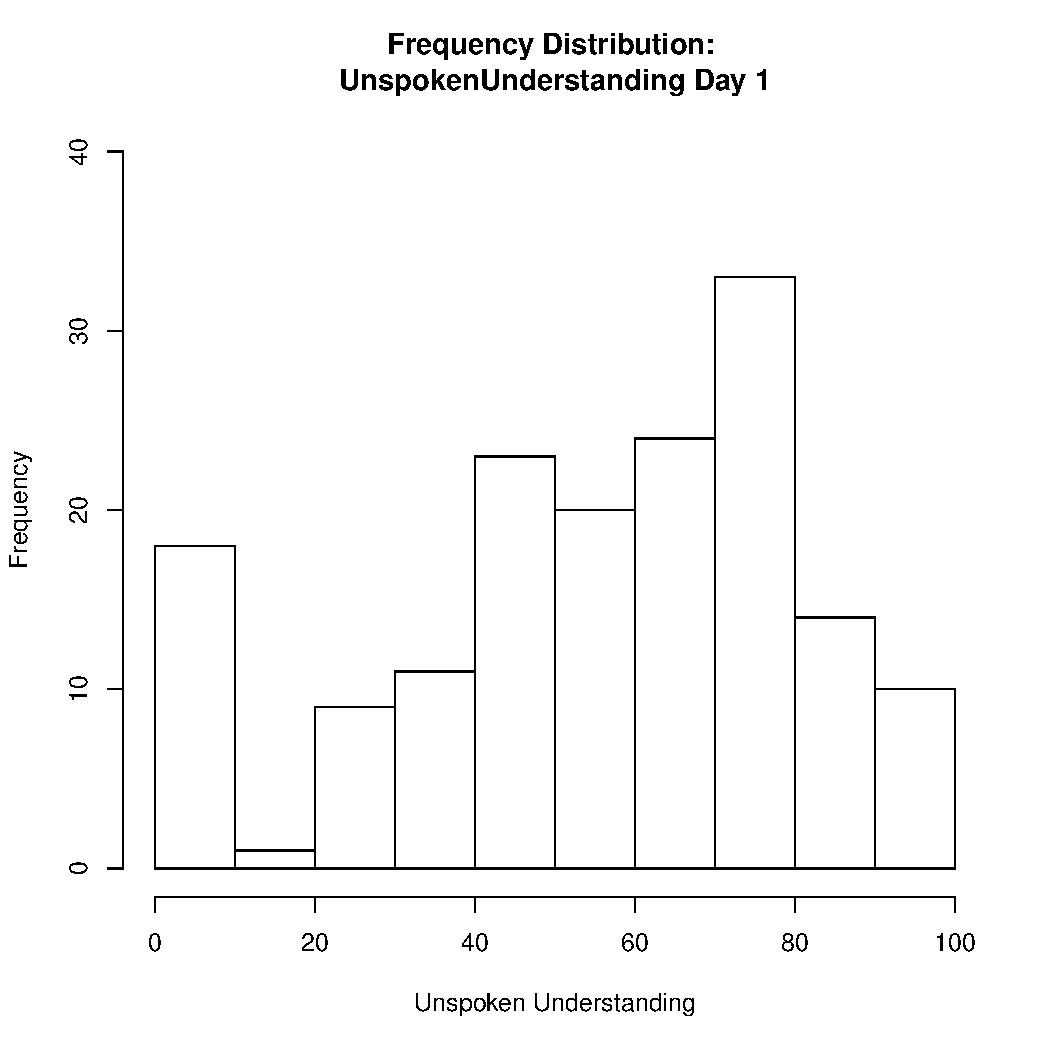
\includegraphics[scale =.4]{../images/distUnspokenUnderstandingDay1.pdf}
  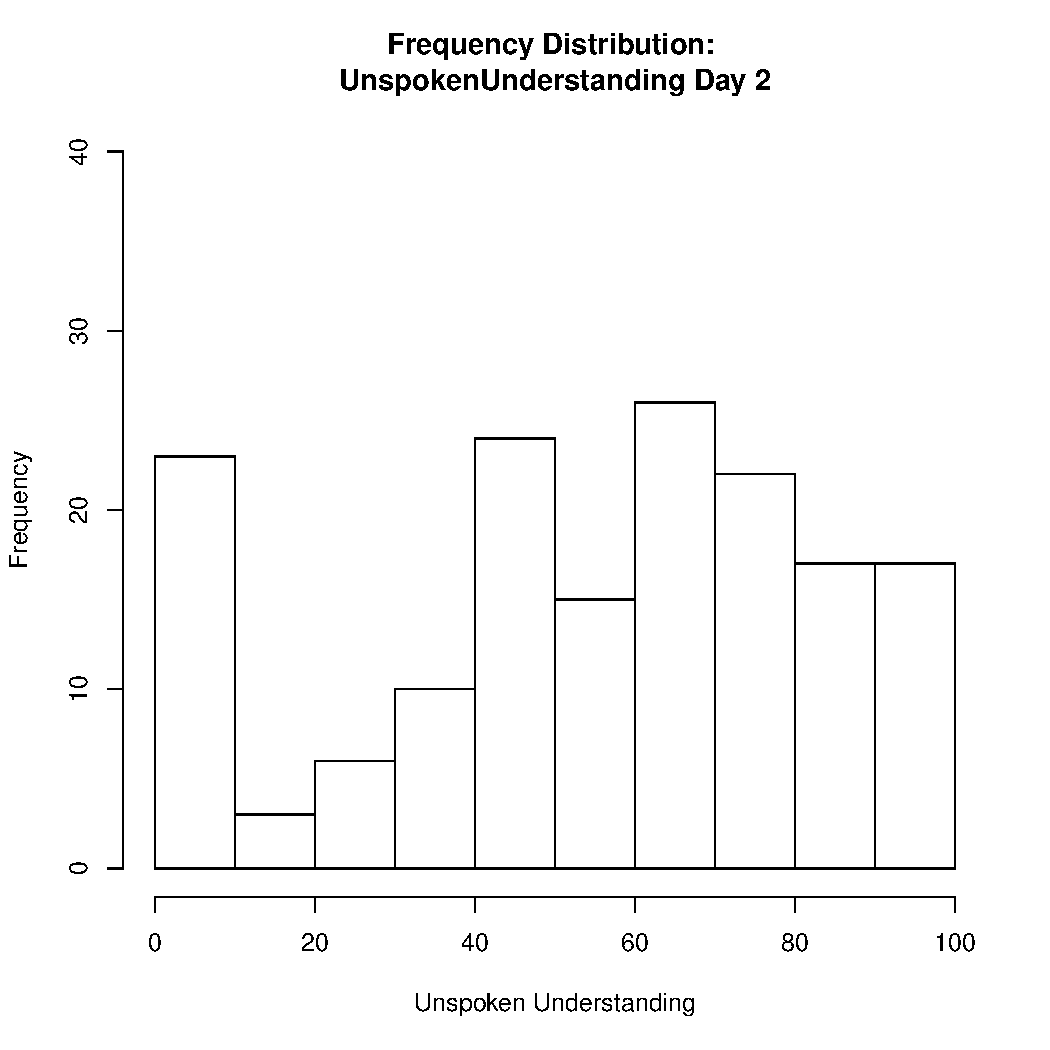
\includegraphics[scale =.4]{../images/distUnspokenUnderstandingDay2.pdf}
  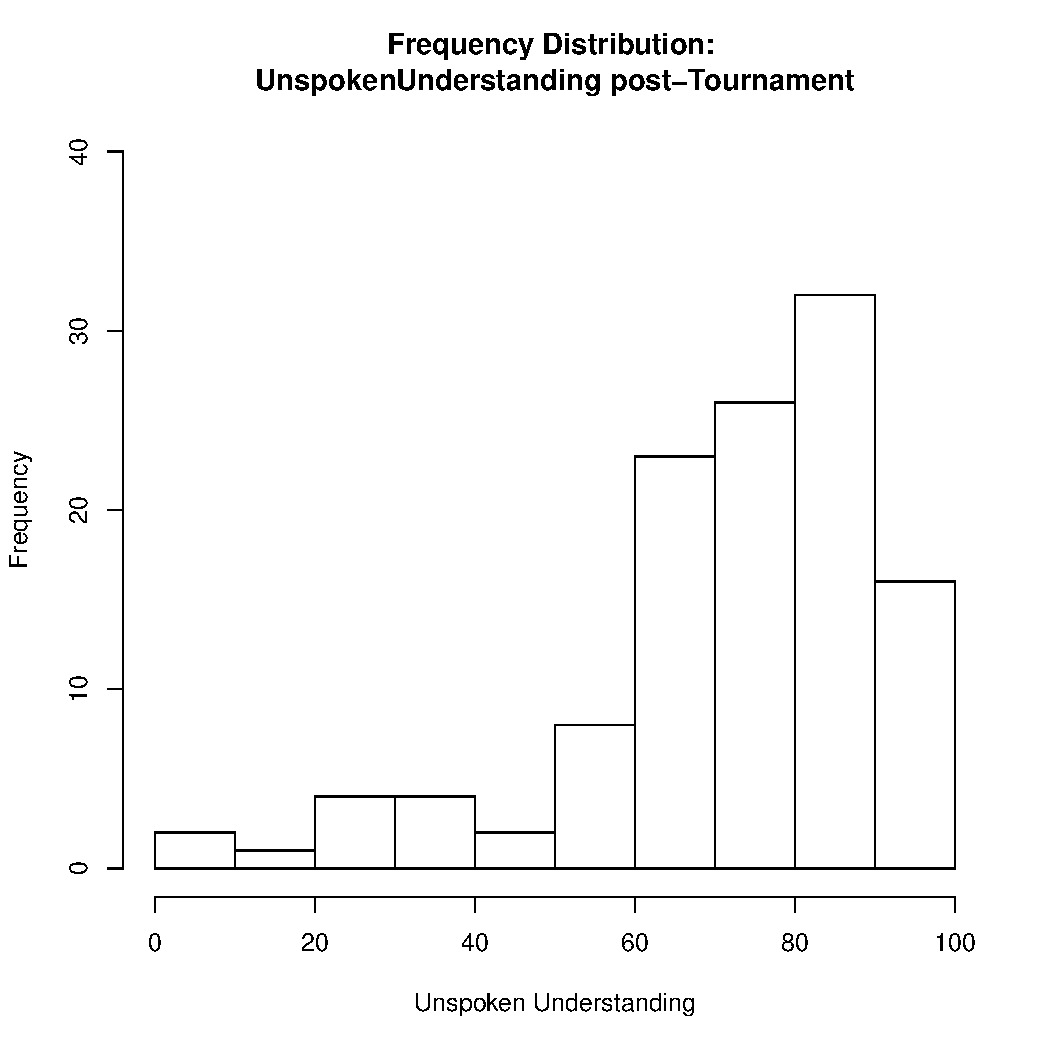
\includegraphics[scale =.4]{../images/distUnspokenUnderstandingPost.pdf}
  \caption{Unspoken Understanding Frequency Distributions}
  \label{fig:unspokenUnderstandingDist}
\end{figure}


%generalAtmosphere
\begin{figure}[htbp]
  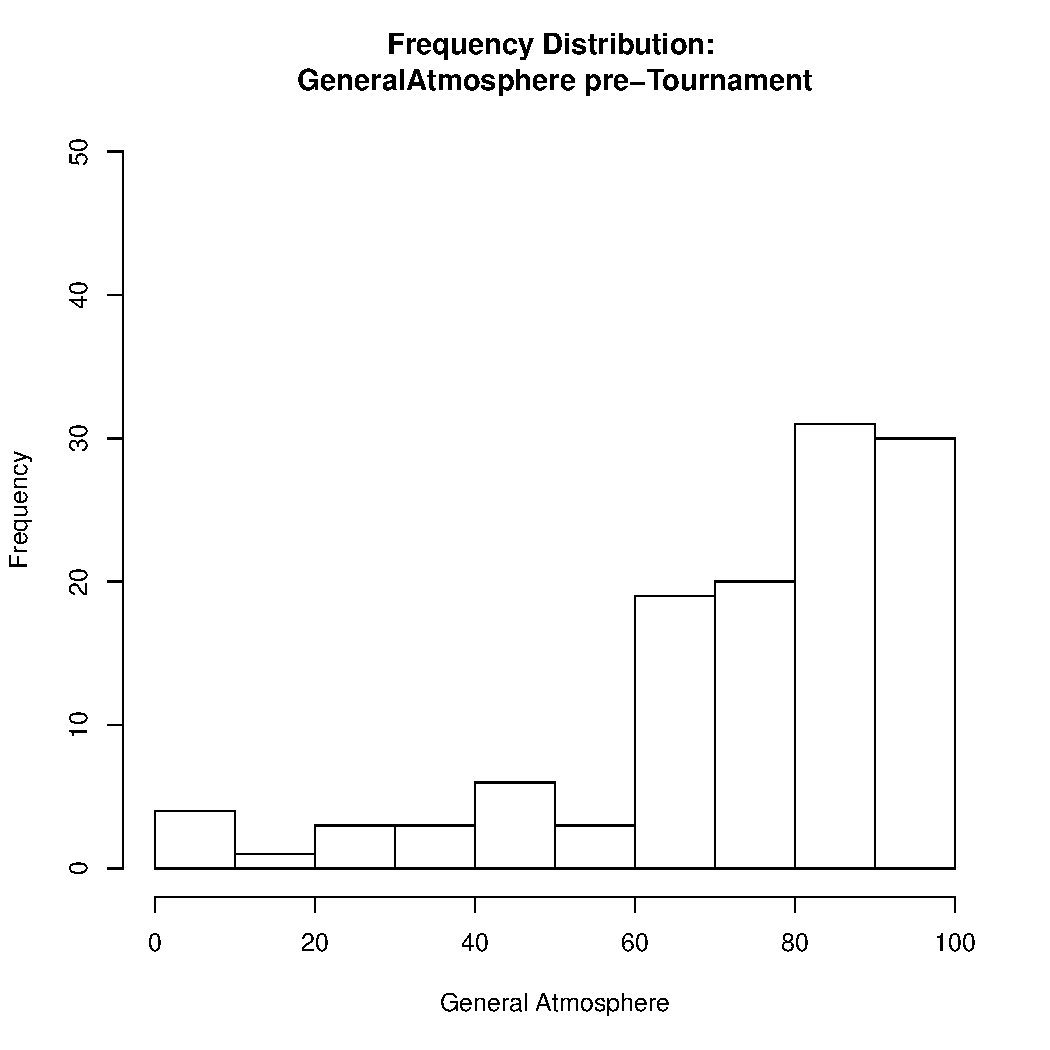
\includegraphics[scale =.4]{../images/distGeneralAtmospherePre.pdf}
  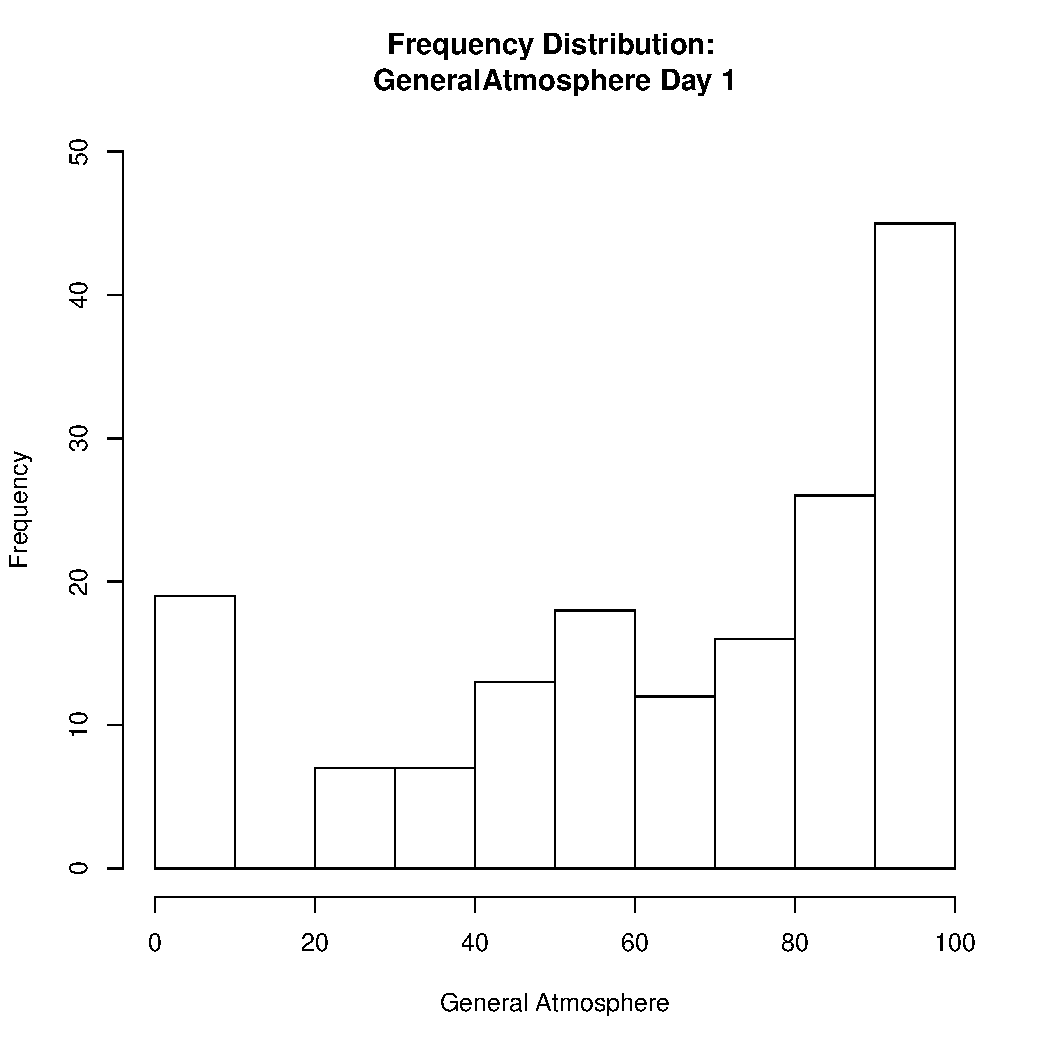
\includegraphics[scale =.4]{../images/distGeneralAtmosphereDay1.pdf}
  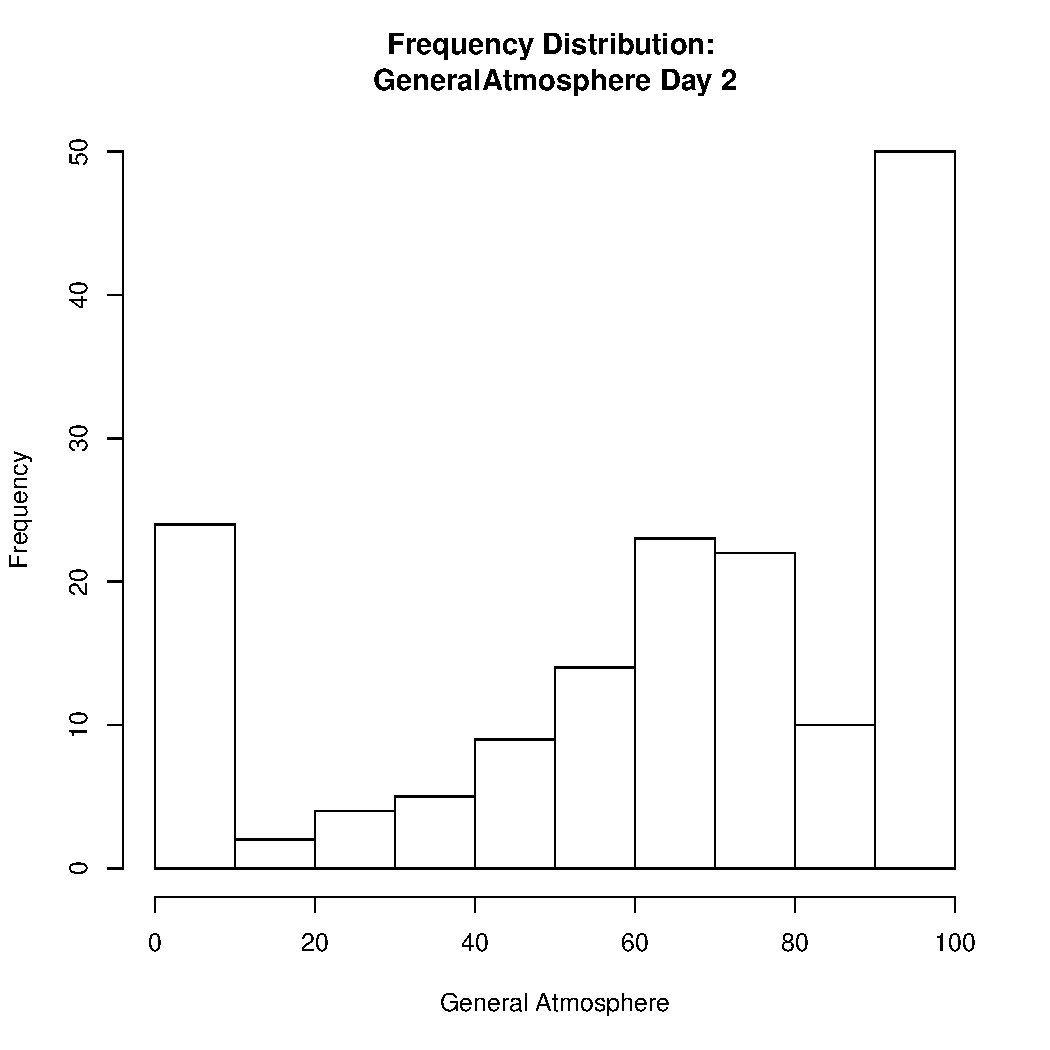
\includegraphics[scale =.4]{../images/distGeneralAtmosphereDay2.pdf}
  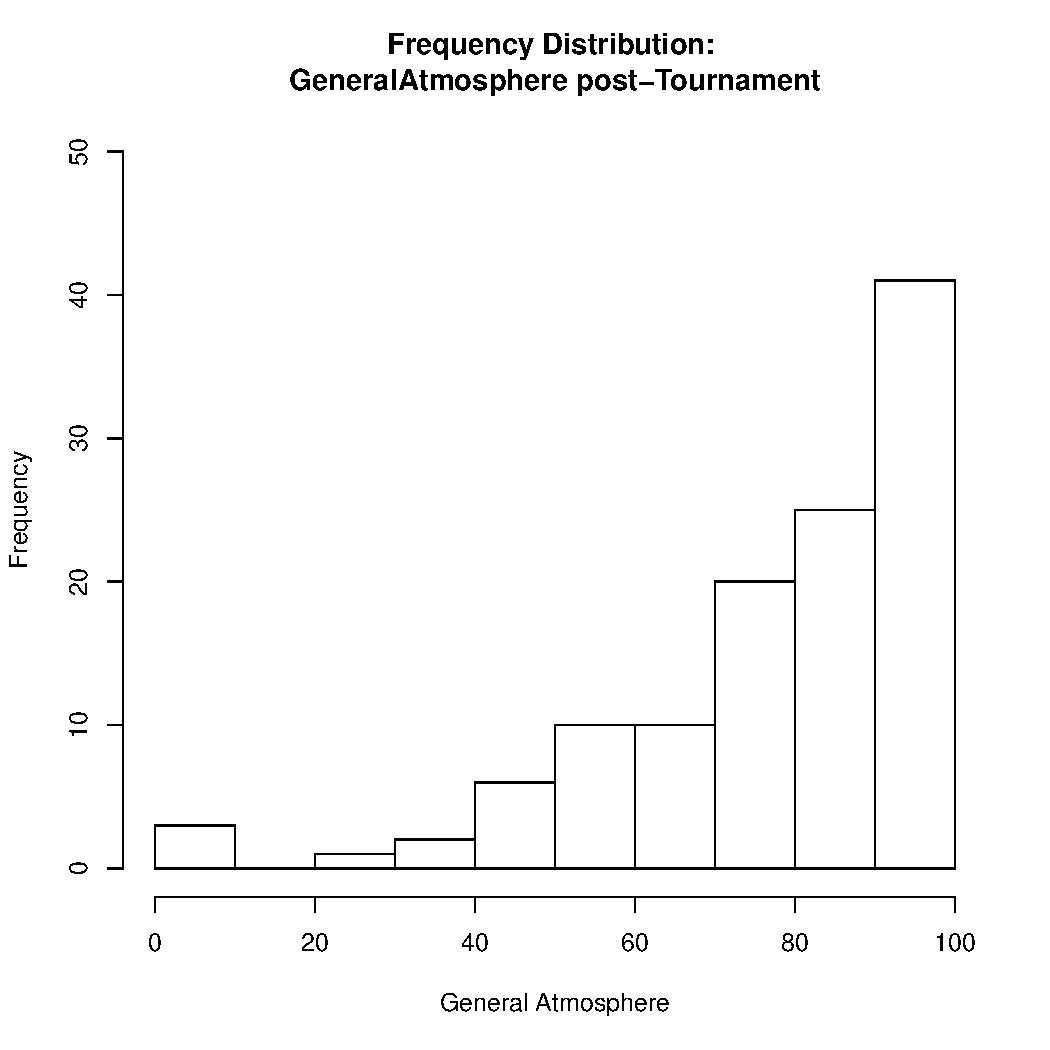
\includegraphics[scale =.4]{../images/distGeneralAtmospherePost.pdf}
  \caption{General Atmosphere Frequency Distributions}
  \label{fig:generalAtmosphereDist}
\end{figure}



\begin{figure}[htbp]
  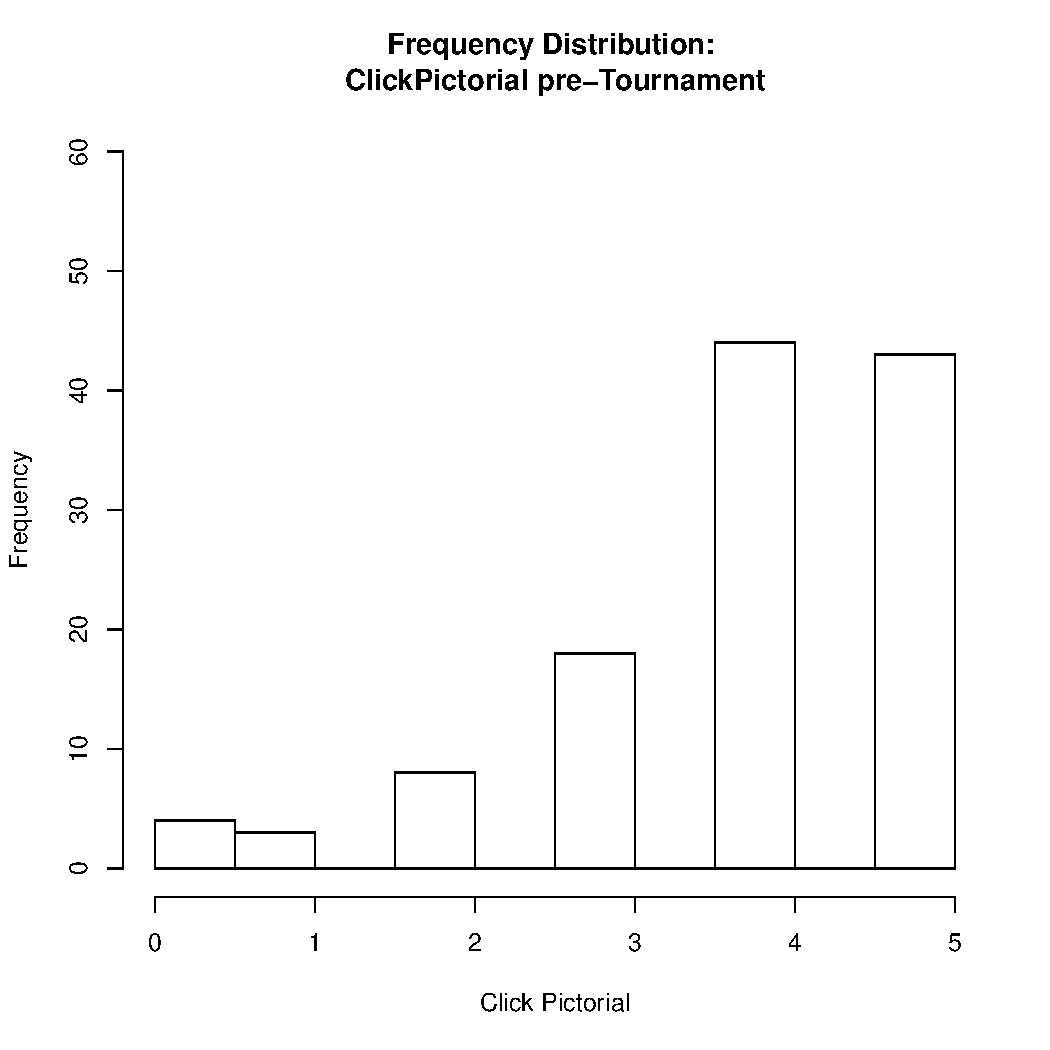
\includegraphics[scale =.4]{../images/distClickPictorialPre.pdf}
  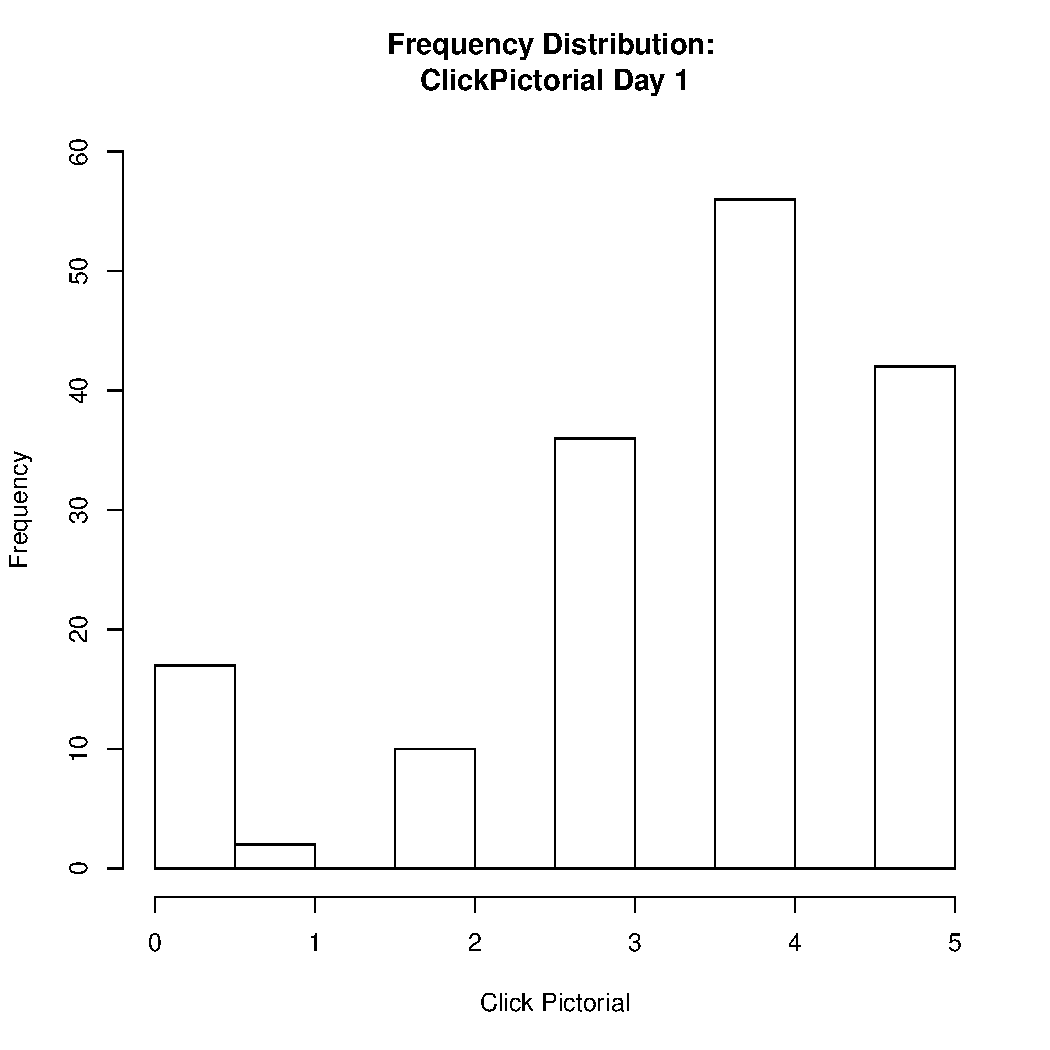
\includegraphics[scale =.4]{../images/distClickPictorialDay1.pdf}
  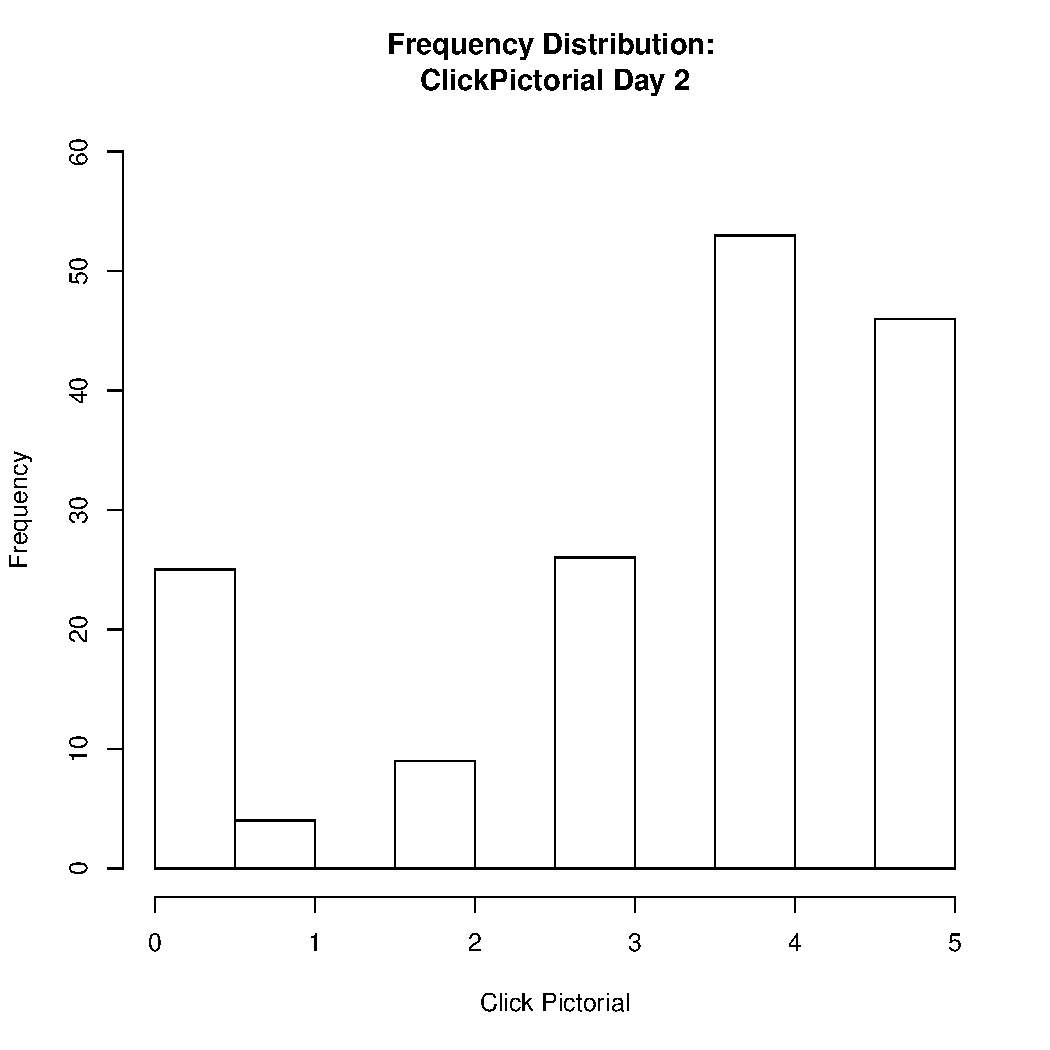
\includegraphics[scale =.4]{../images/distClickPictorialDay2.pdf}
  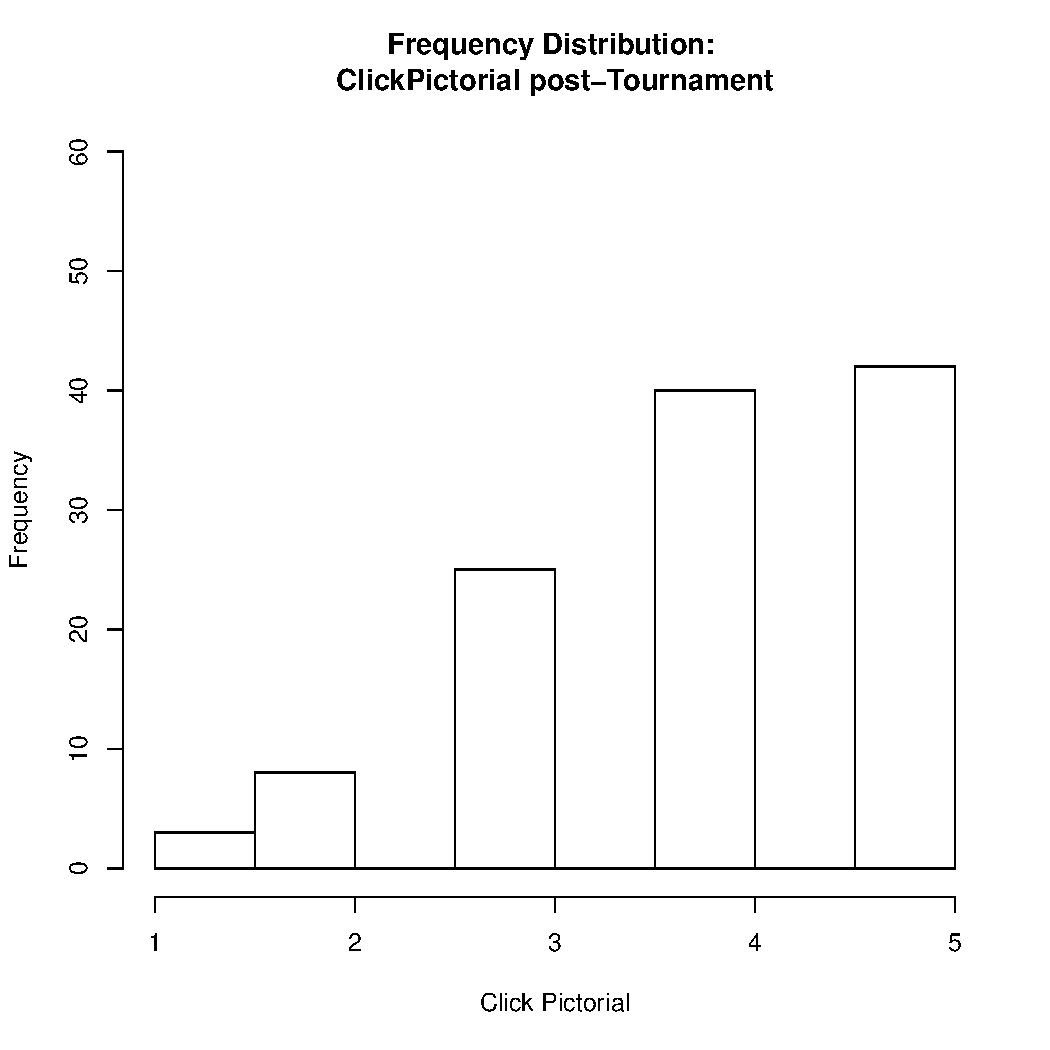
\includegraphics[scale =.4]{../images/distClickPictorialPost.pdf}
  \caption{Click Pictorial Frequency Distributions}
  \label{fig:clickPictorialDist}
\end{figure}


%Bonding:
%emotionalSupport

\begin{figure}[htbp]
  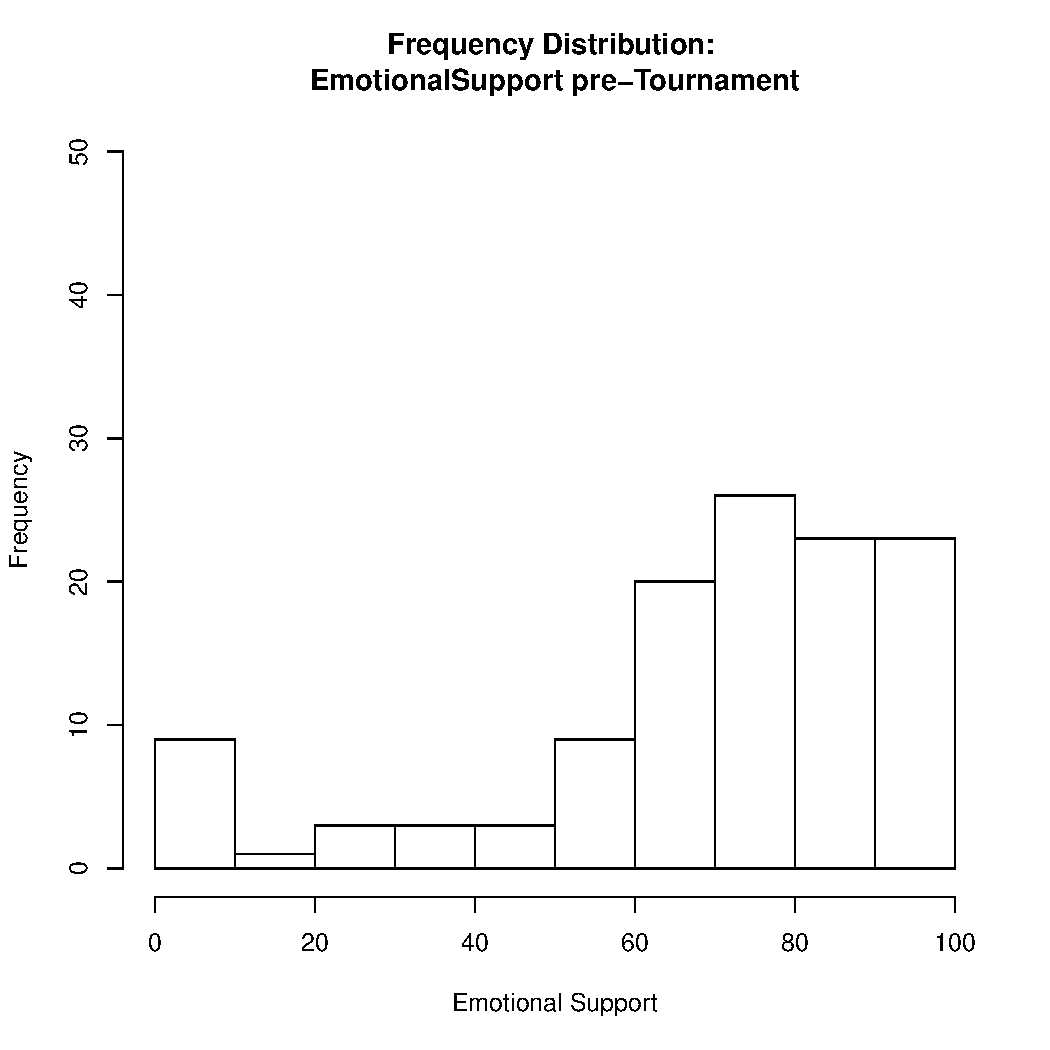
\includegraphics[scale =.4]{../images/distEmotionalSupportPre.pdf}
  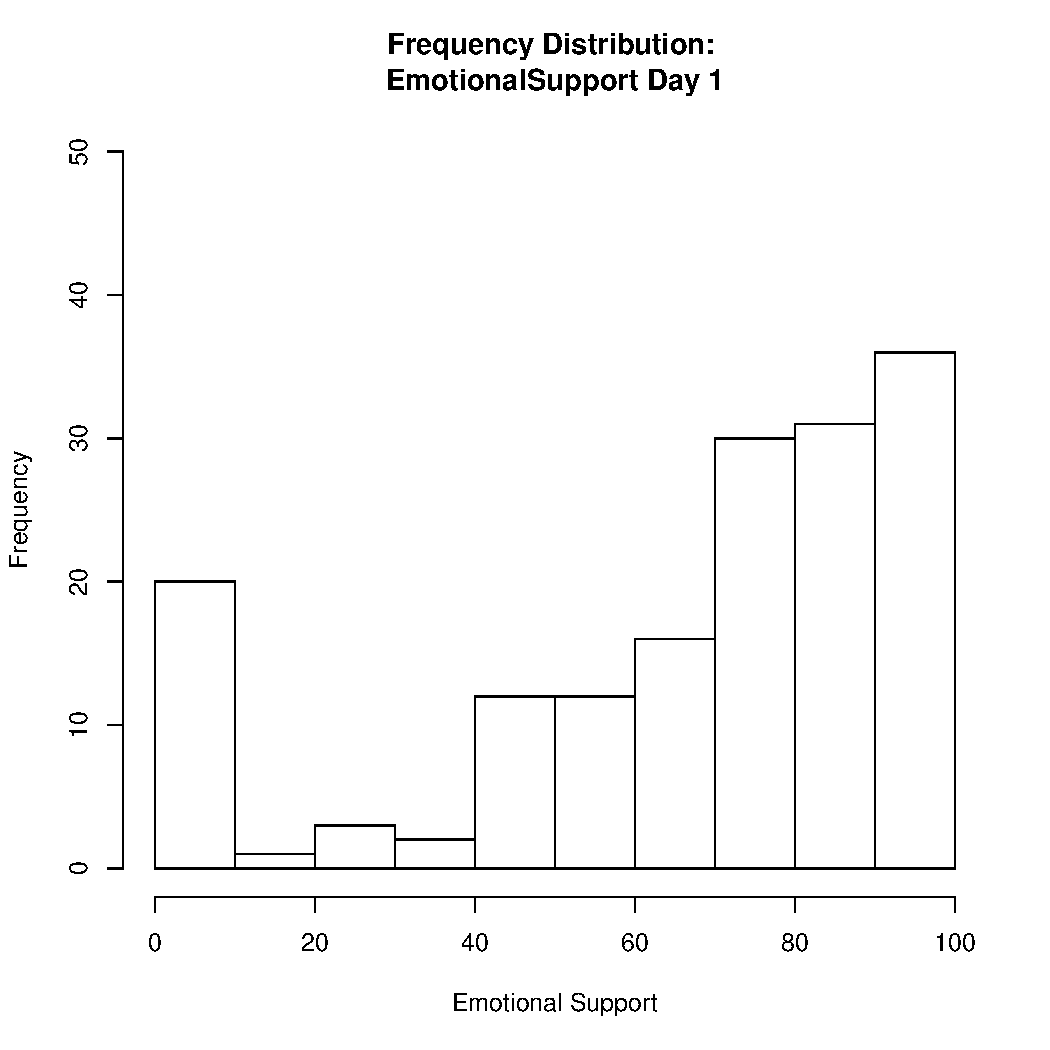
\includegraphics[scale =.4]{../images/distEmotionalSupportDay1.pdf}
  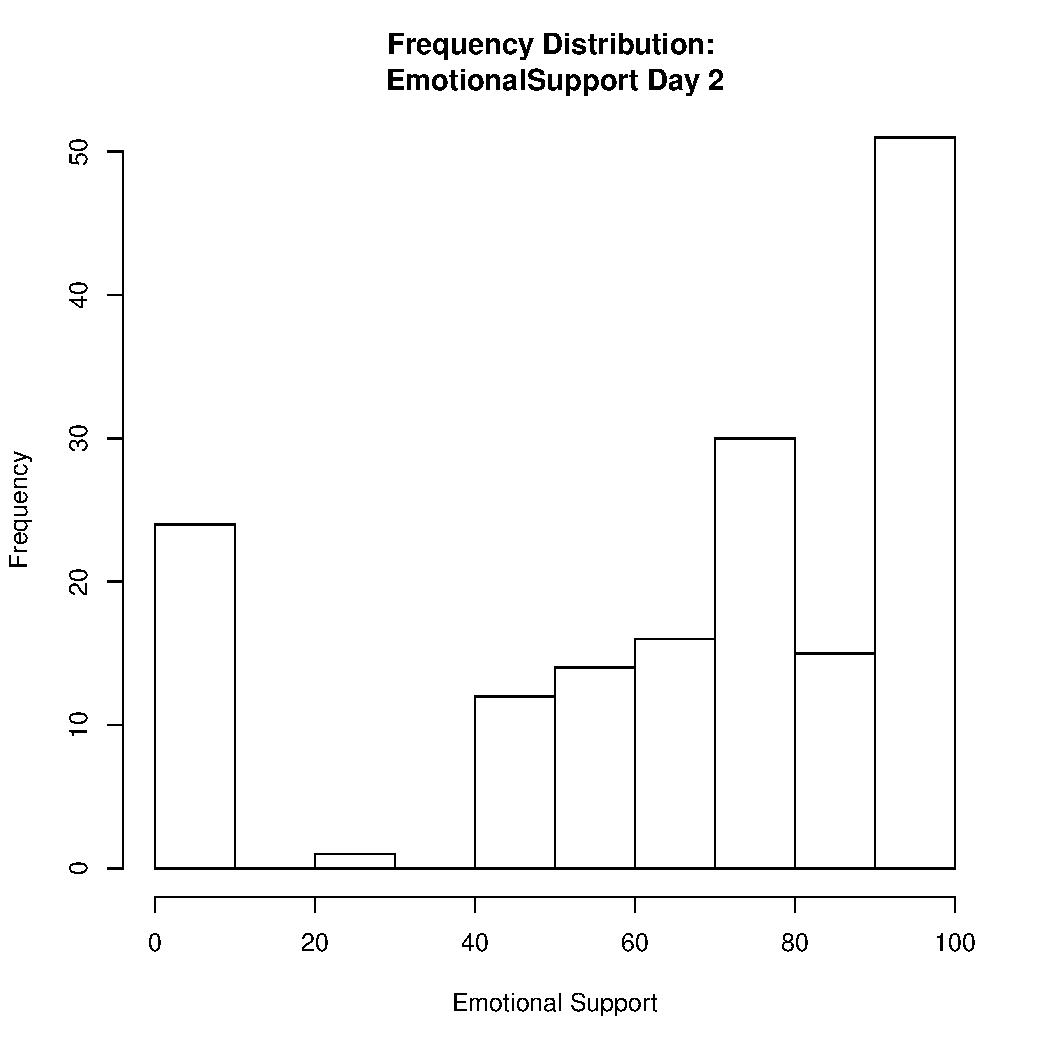
\includegraphics[scale =.4]{../images/distEmotionalSupportDay2.pdf}
  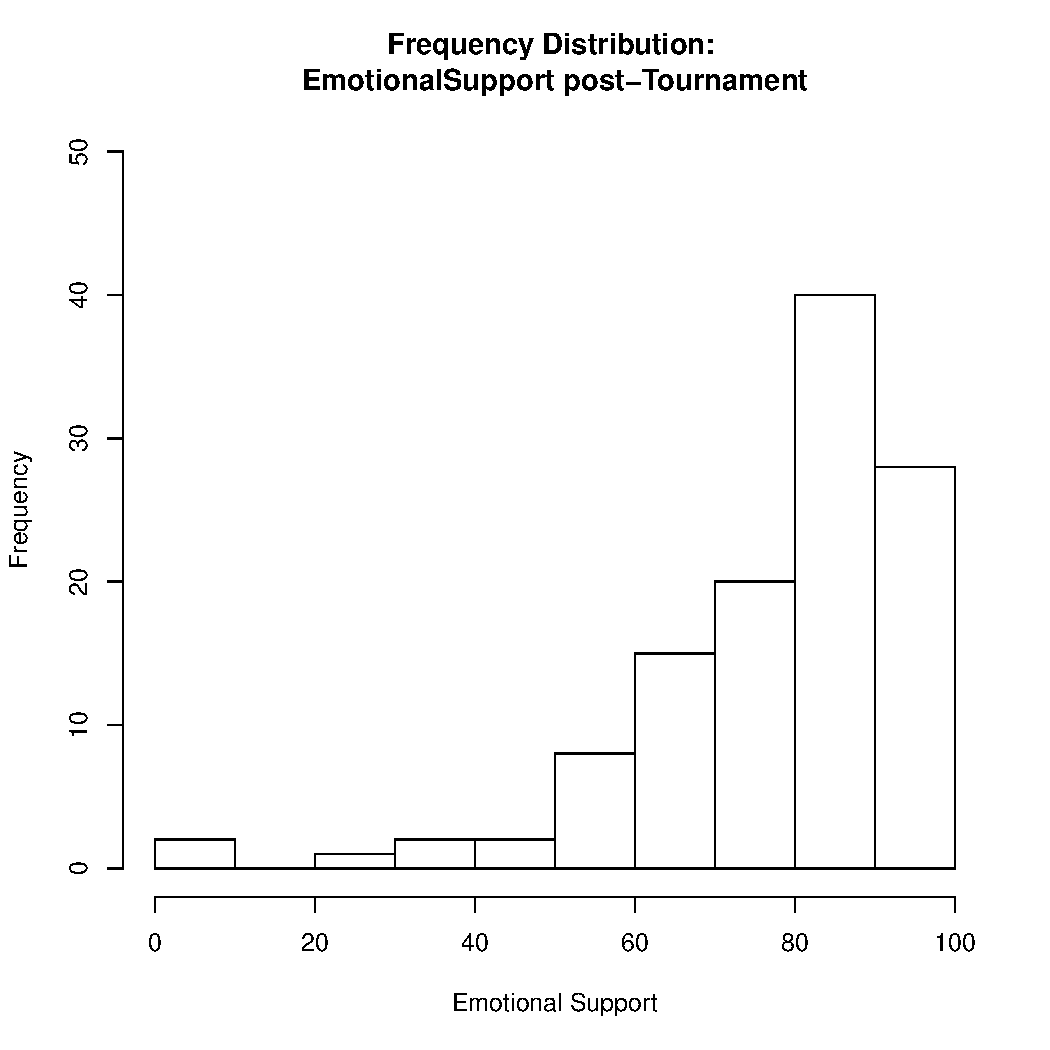
\includegraphics[scale =.4]{../images/distEmotionalSupportPost.pdf}
  \caption{Emotional Support Frequency Distributions}
  \label{fig:emotionalSupportDist}
\end{figure}


%sharedGoal

\begin{figure}[htbp]
  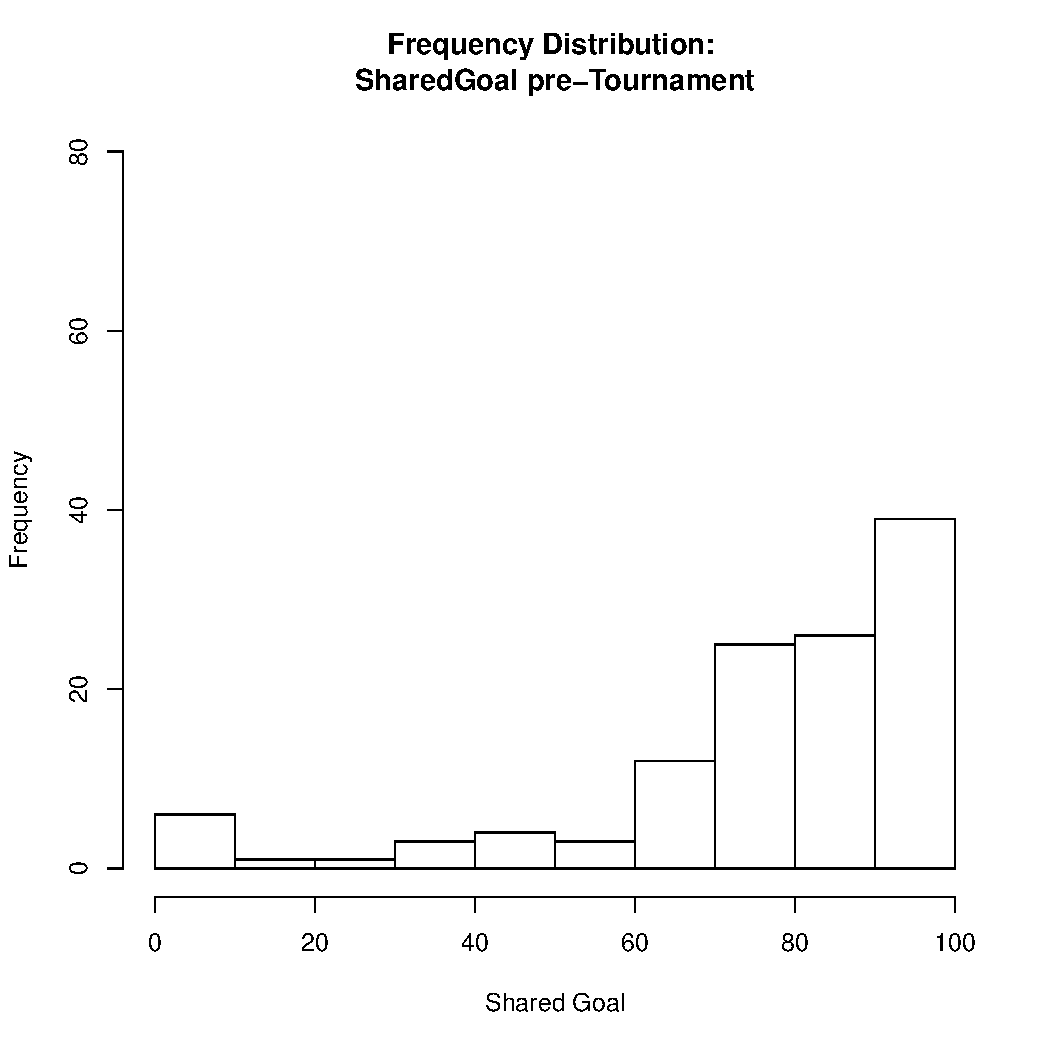
\includegraphics[scale =.4]{../images/distSharedGoalPre.pdf}
  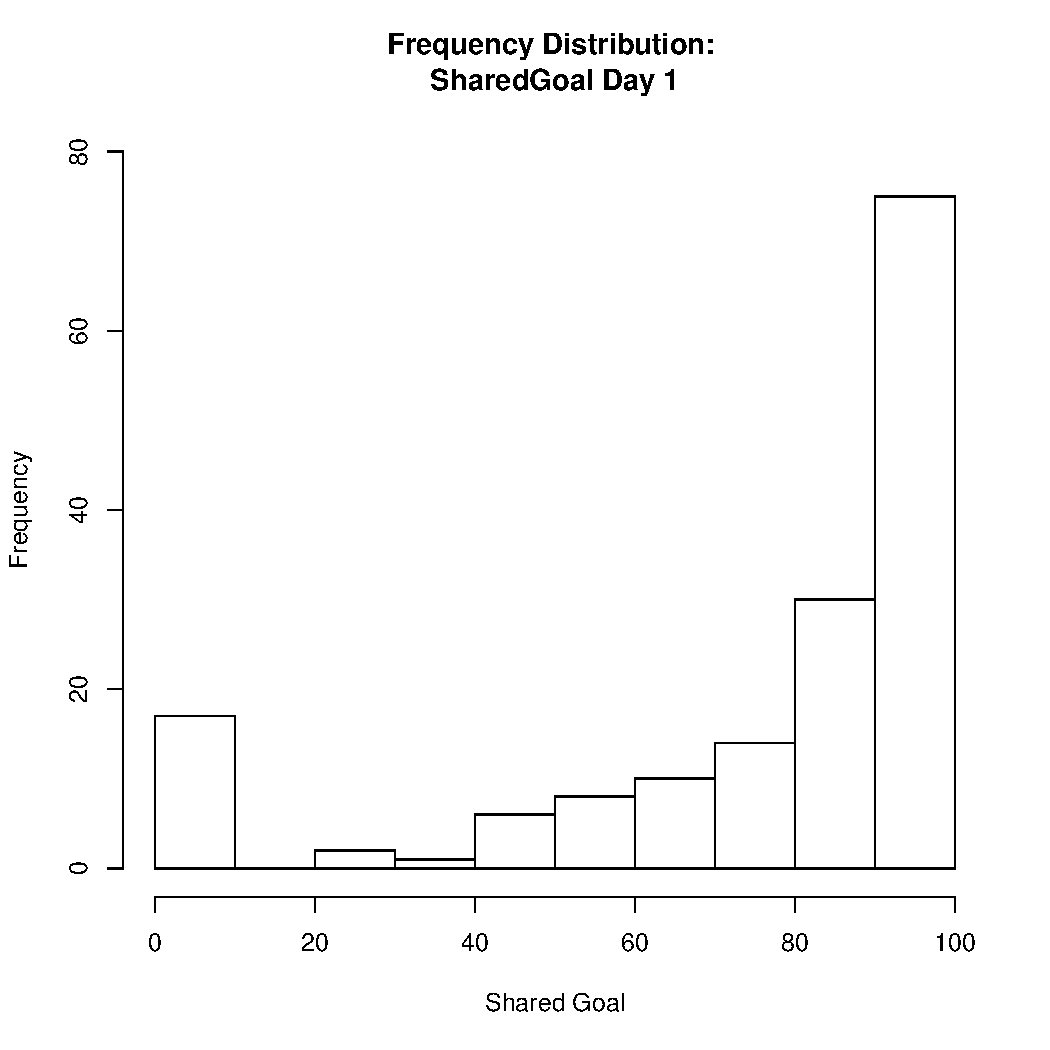
\includegraphics[scale =.4]{../images/distSharedGoalDay1.pdf}
  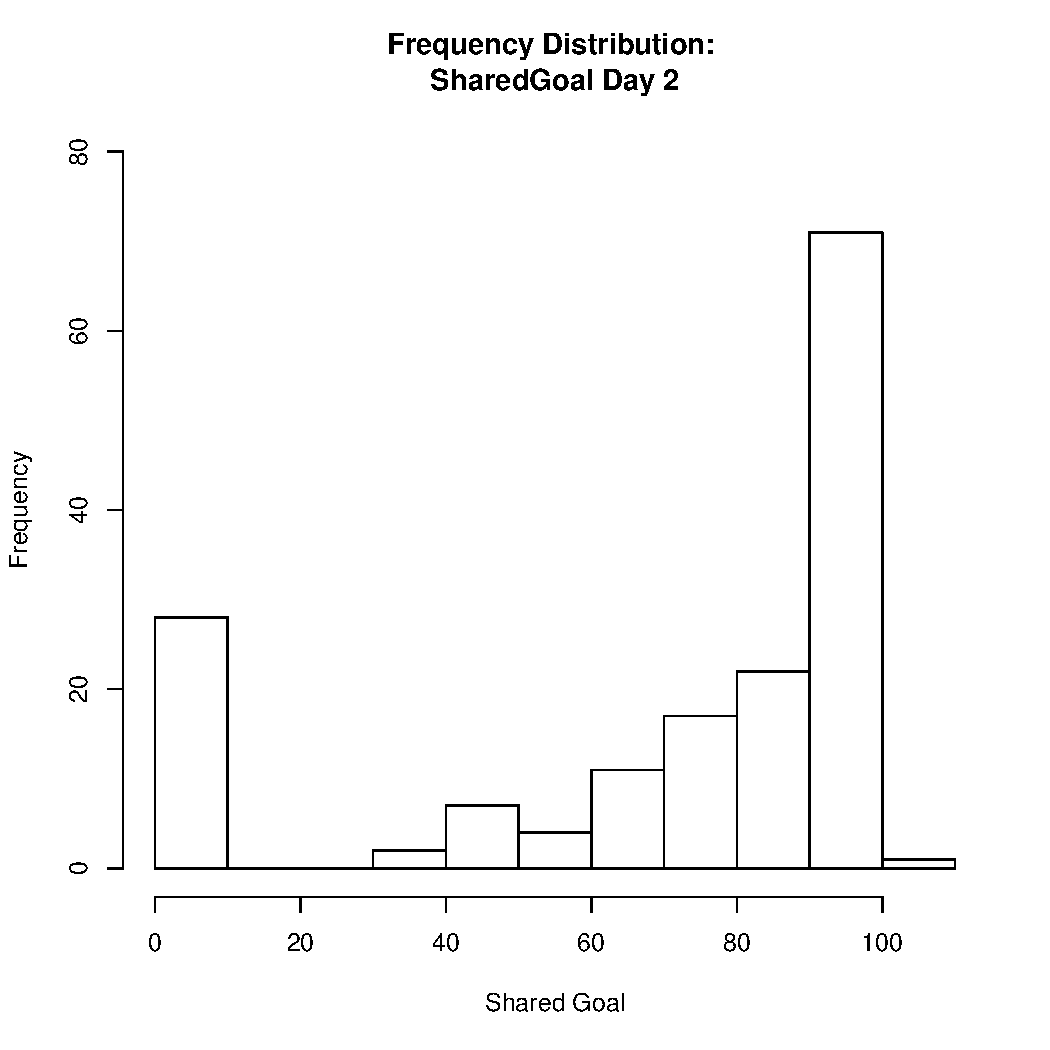
\includegraphics[scale =.4]{../images/distSharedGoalDay2.pdf}
  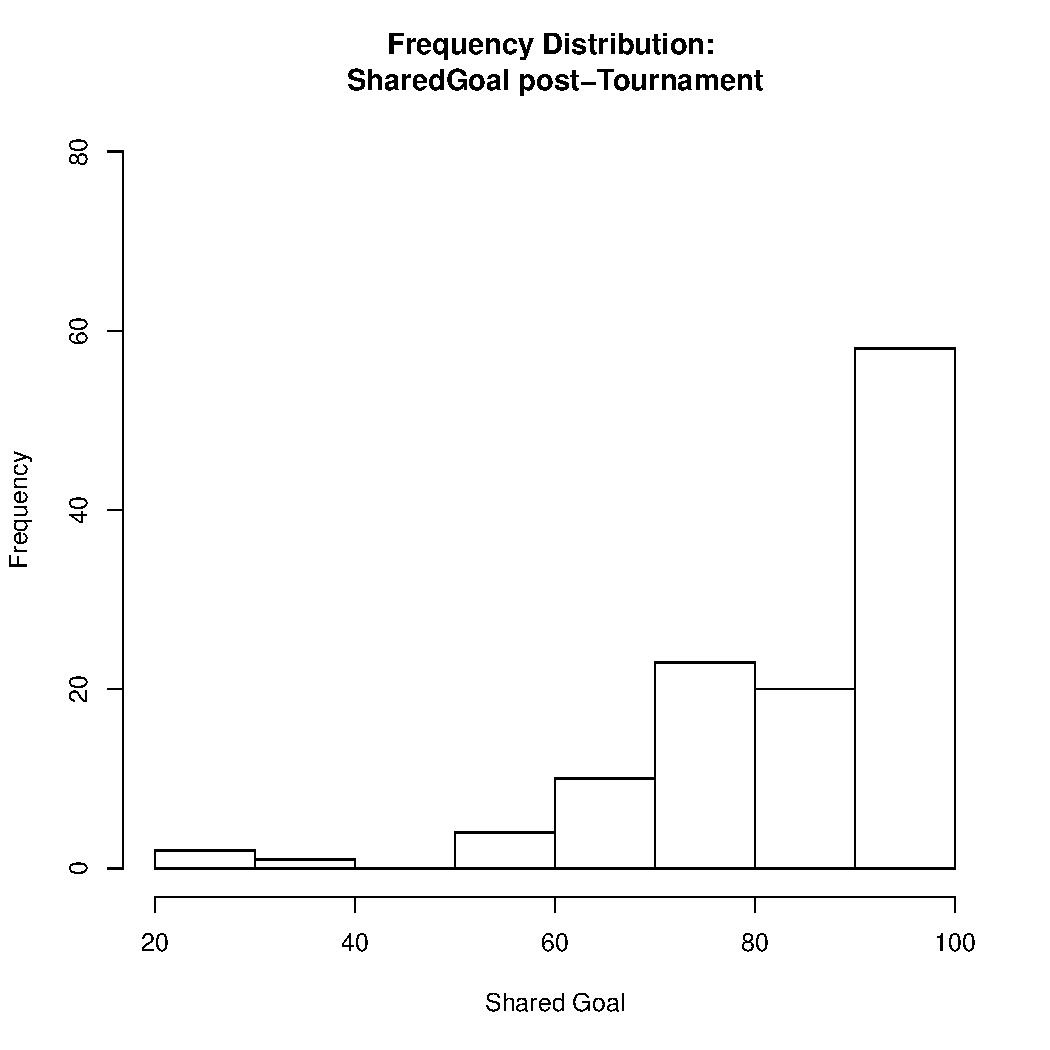
\includegraphics[scale =.4]{../images/distSharedGoalPost.pdf}
  \caption{Shared Goal Frequency Distributions}
  \label{fig:sharedGoalDist}
\end{figure}


% fusionPictorial
\begin{figure}[htbp]
  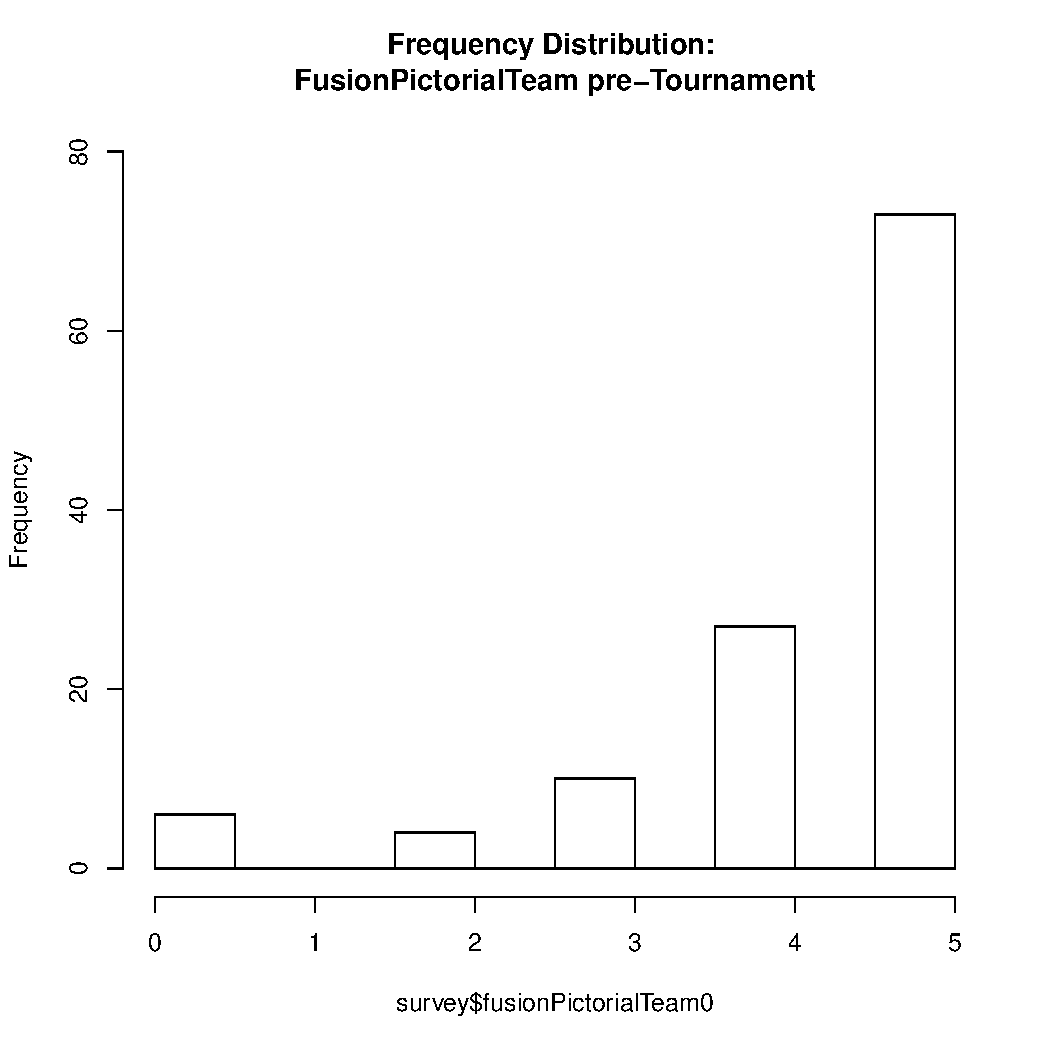
\includegraphics[scale =.4]{../images/distFusionPictorialTeamPre.pdf}
  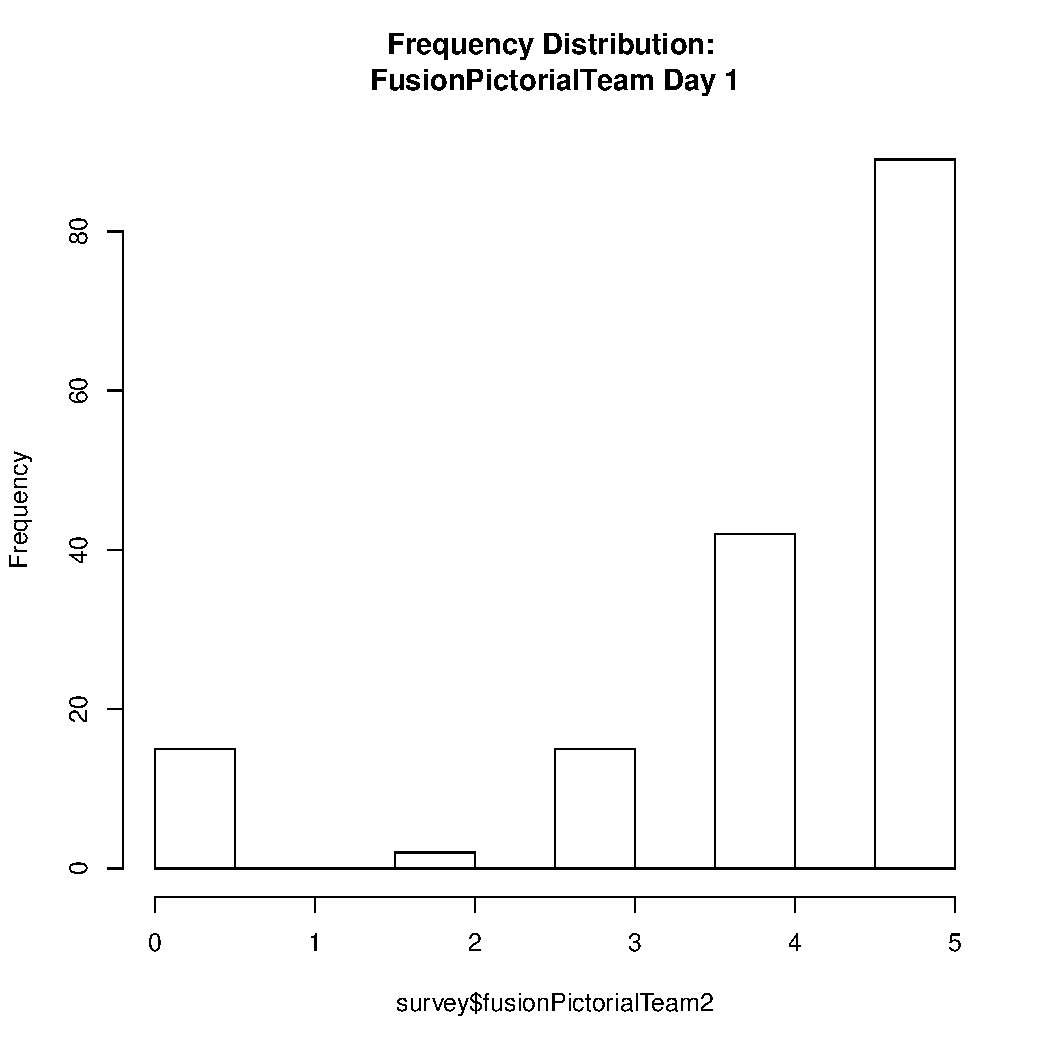
\includegraphics[scale =.4]{../images/distFusionPictorialTeamDay1.pdf}
  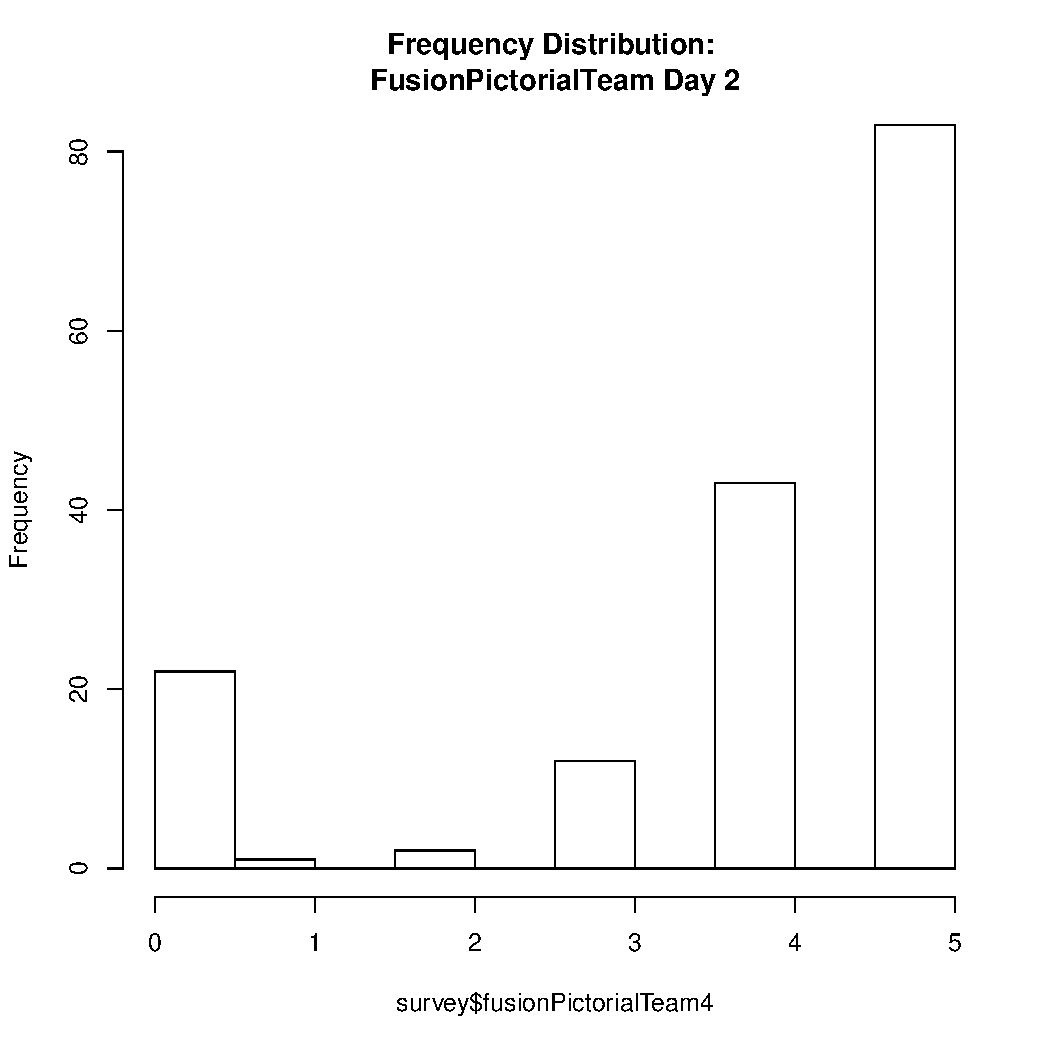
\includegraphics[scale =.4]{../images/distFusionPictorialTeamDay2.pdf}
  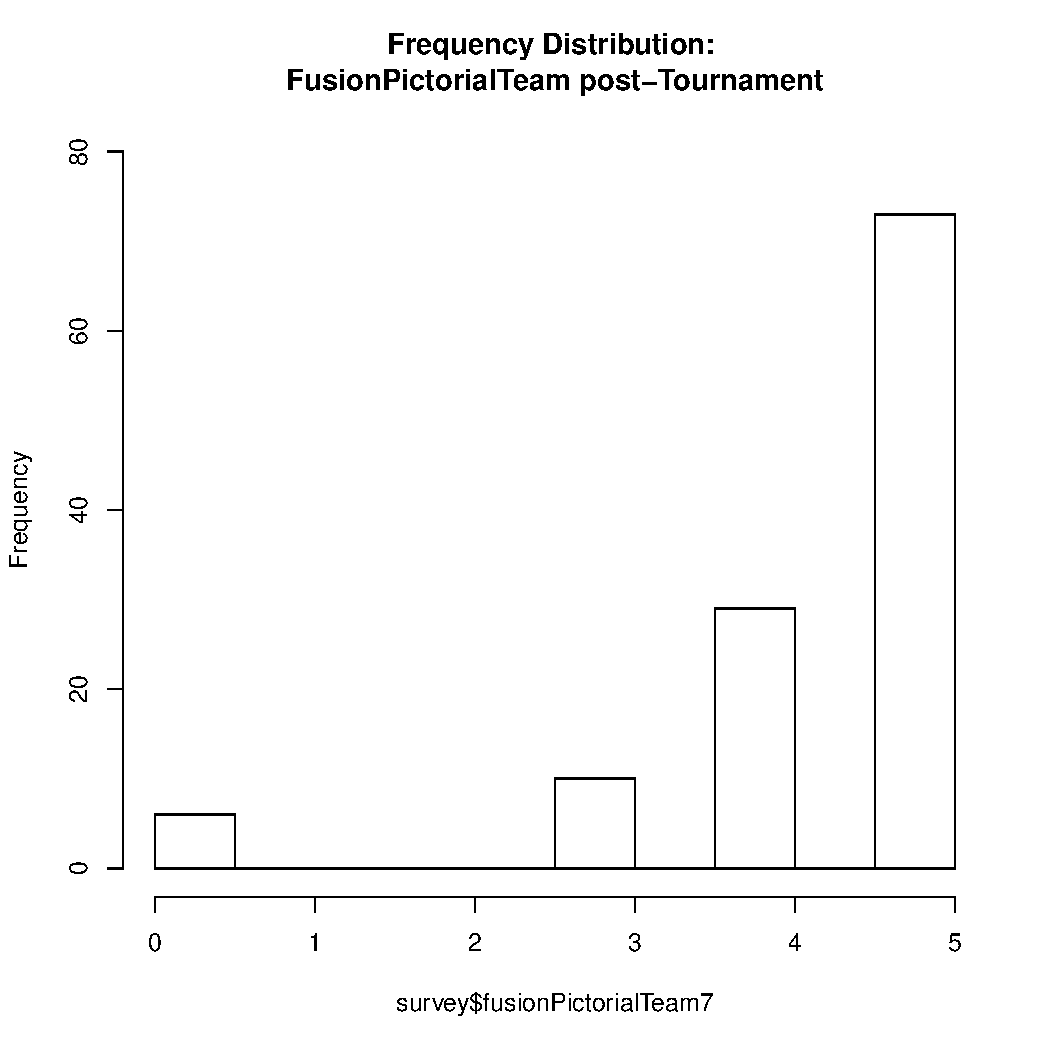
\includegraphics[scale =.4]{../images/distFusionPictorialTeamPost.pdf}
  \caption{Fusion Pictorial Frequency Distributions}
  \label{fig:fusionPictorialDist}
\end{figure}



%fatigue
\begin{figure}[htbp]
  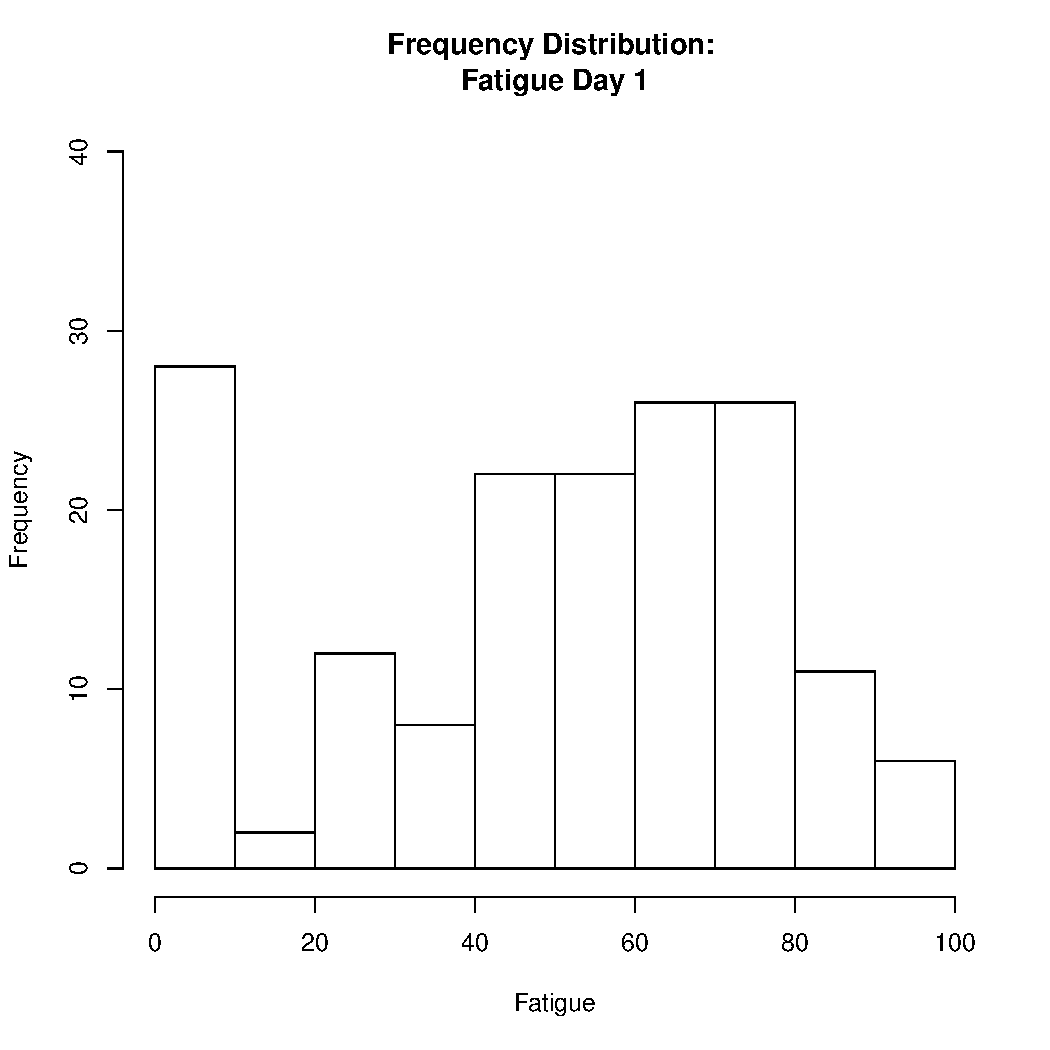
\includegraphics[scale =.4]{../images/distFatigueDay1.pdf}
  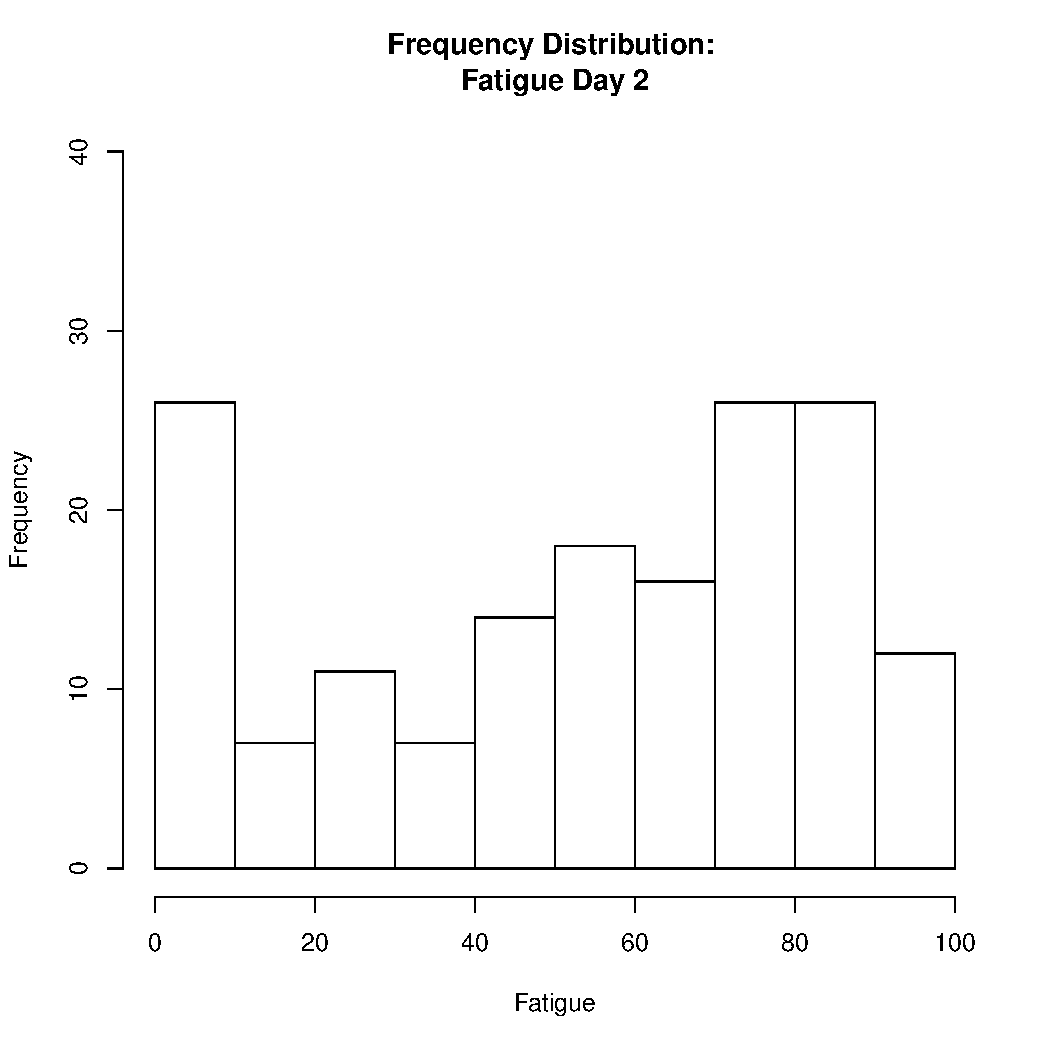
\includegraphics[scale =.4]{../images/distFatigueDay2.pdf}
  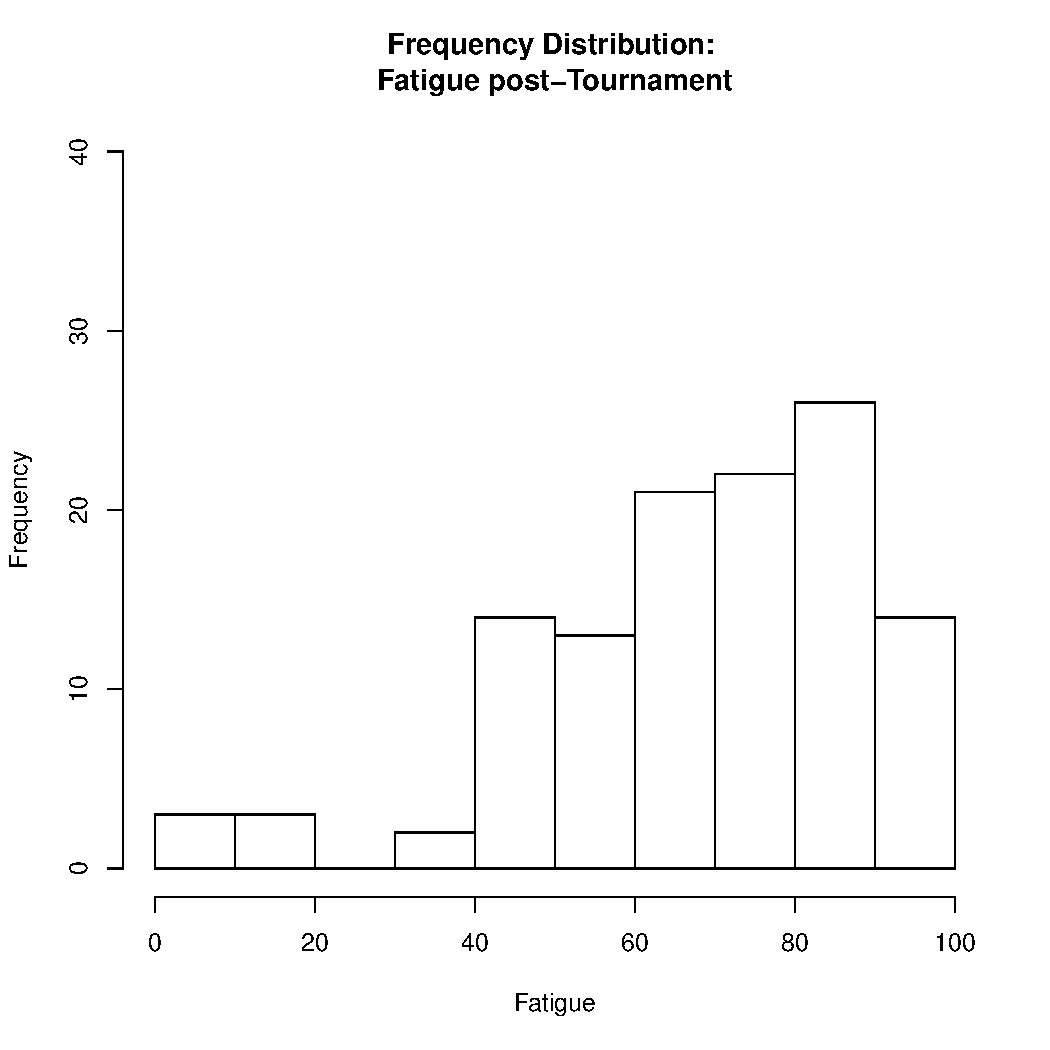
\includegraphics[scale =.4]{../images/distFatiguePost.pdf}
  \caption{Fatigue Frequency Distributions}
  \label{fig:fatigueDist}
\end{figure}



%prpe
\begin{figure}[htbp]
  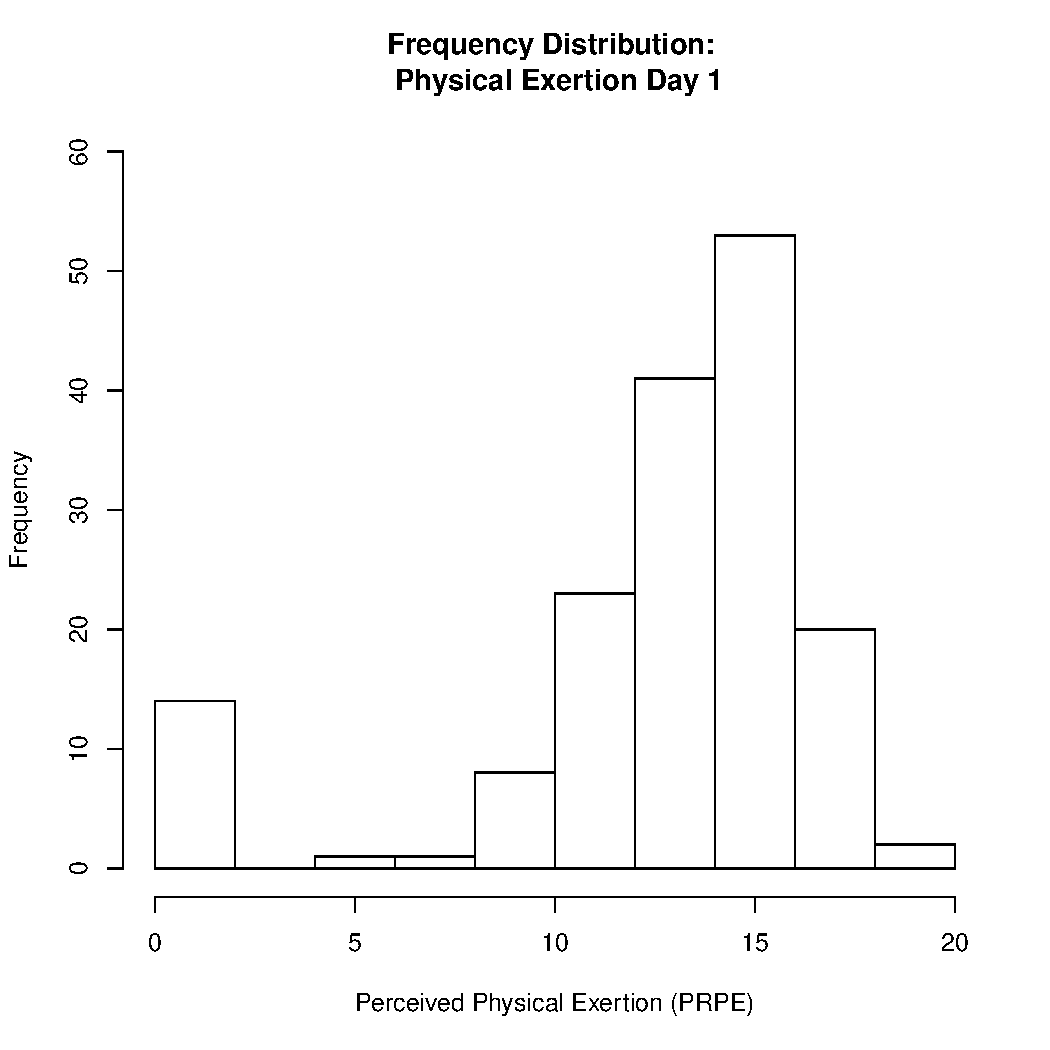
\includegraphics[scale =.4]{../images/distPrpeDay1.pdf}
  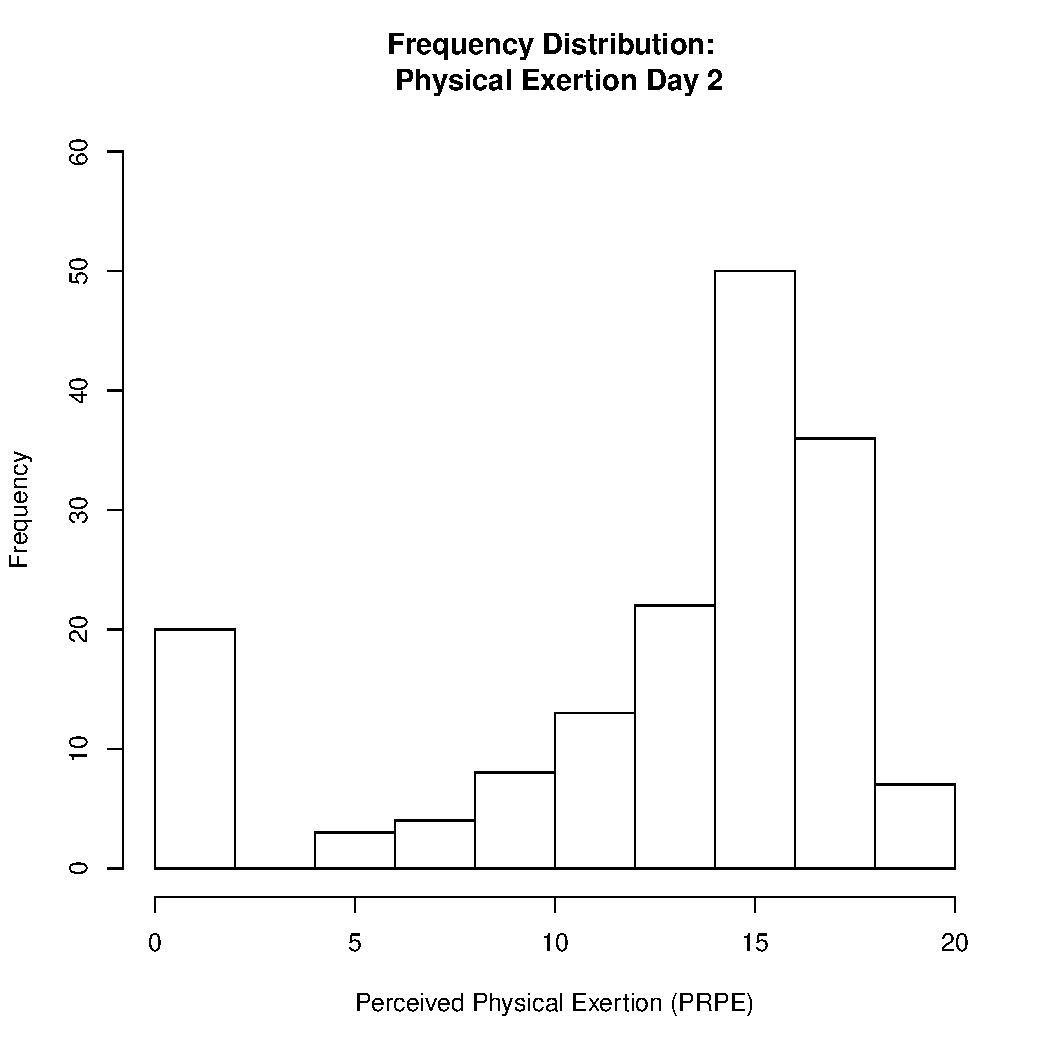
\includegraphics[scale =.4]{../images/distPrpeDay2.pdf}
  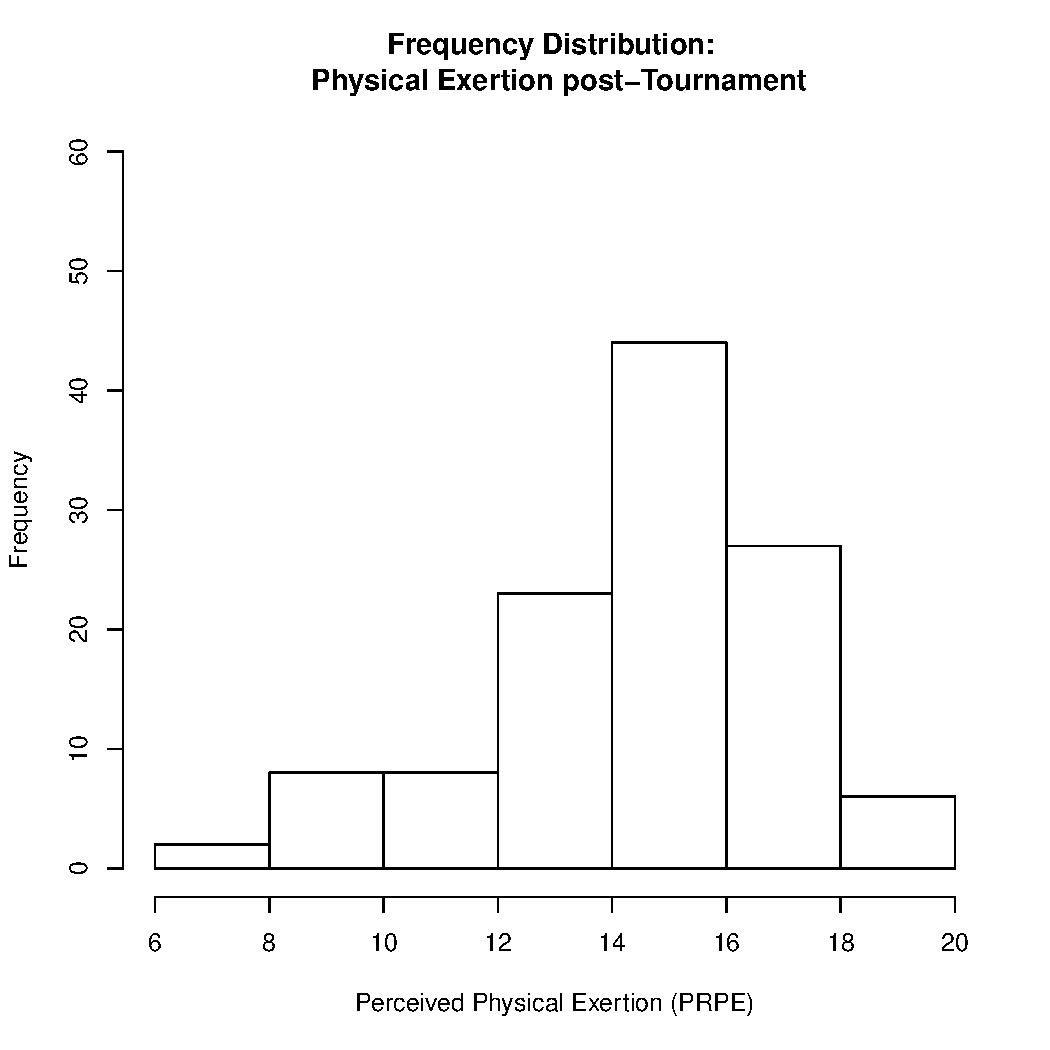
\includegraphics[scale =.4]{../images/distPrpePost.pdf}
  \caption{Perceived Physical Exertion Frequency Distribution}
  \label{fig:prpeDist}
\end{figure}



%mental

\begin{figure}[htbp]
  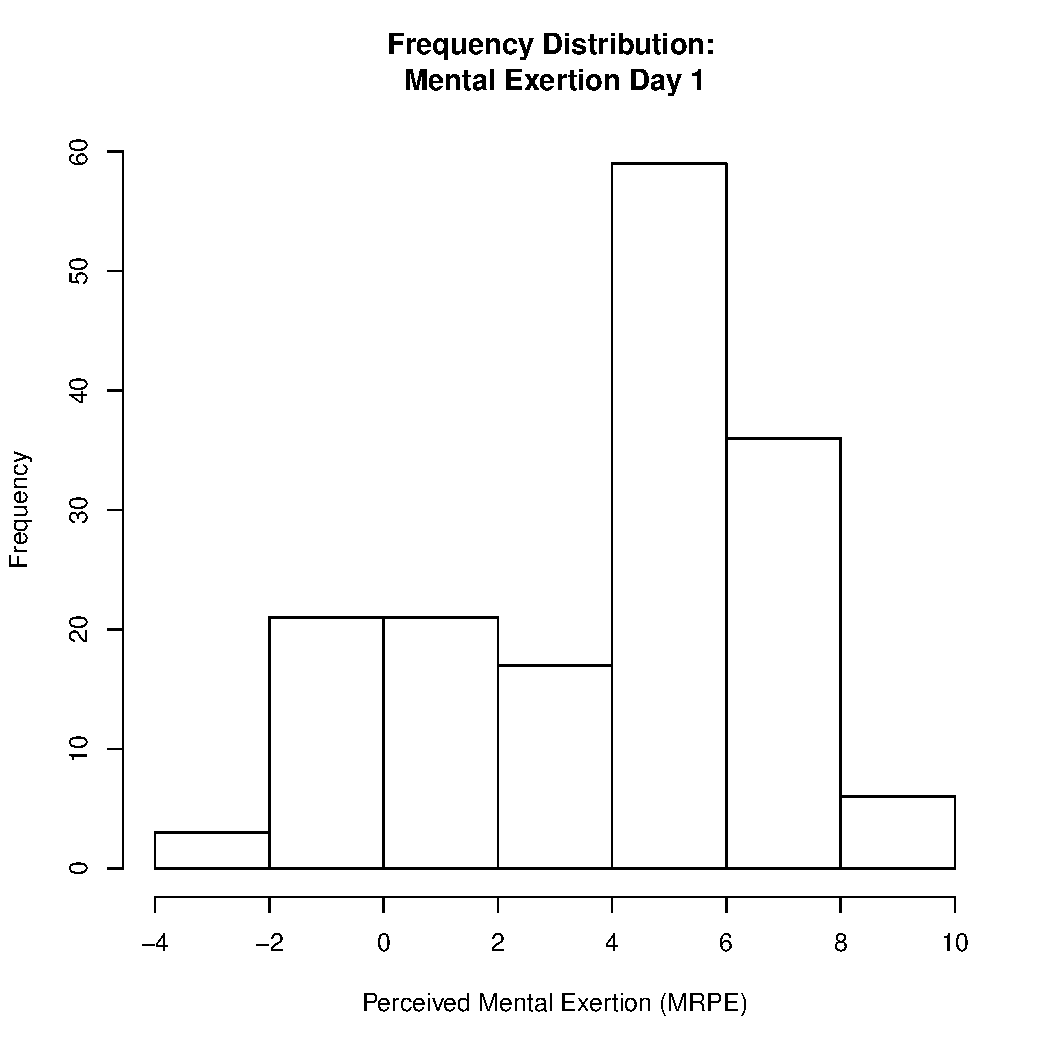
\includegraphics[scale =.4]{../images/distMentalDay1.pdf}
  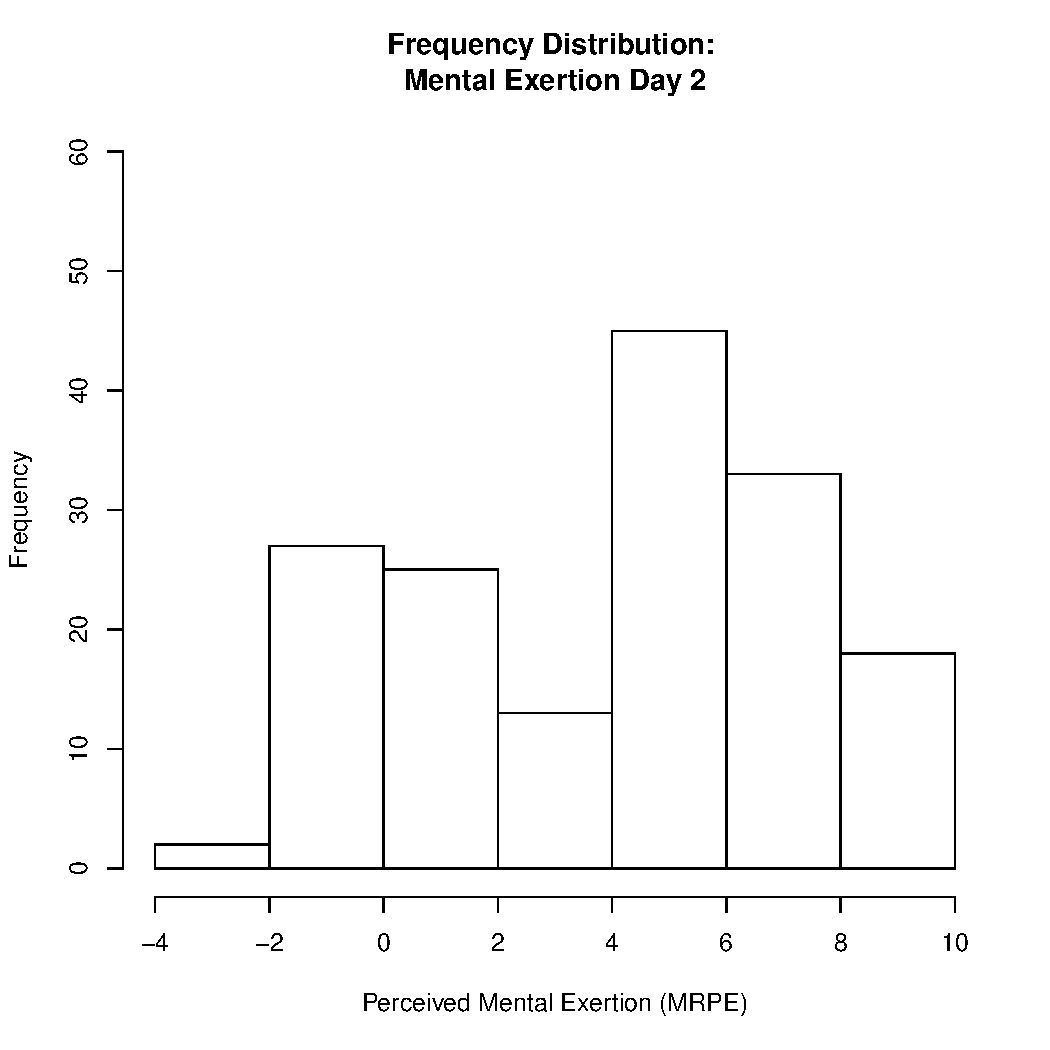
\includegraphics[scale =.4]{../images/distMentalDay2.pdf}
  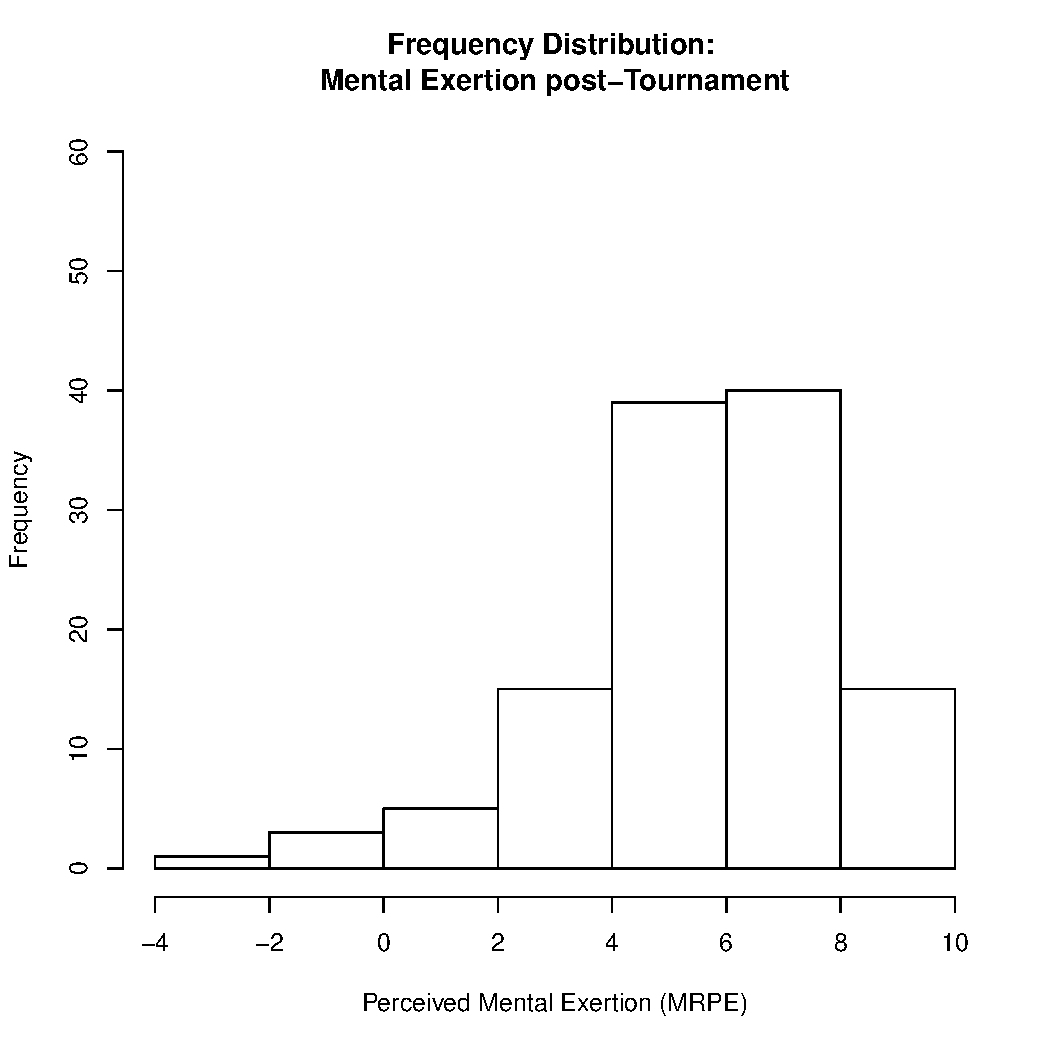
\includegraphics[scale =.4]{../images/distMentalPost.pdf}
  \caption{Perceived Mental Exertion Frequency Distributions}
  \label{fig:mentalDist}
\end{figure}




This observed pattern has a number of potential explanations. First, the pattern of extremely low responses could be an indication of athletes’ disappointment with individual and team performance immediately following games. To test this interpretation, correlations between game result (win or loss) immediately prior to being surveyed and responses for performance, team click, social bonding, and fatigue were examined using linear regressions.  The relationship between game outcome and Team Performance Expectations for all athletes who participated in the Day 1 was not significant, $F(1,159) = 2.1 SE = 30.32, p = .15$; $\beta = 6.92, SE = 4.78, t = 1.45 p = .15.$  Of those athletes who scored zero for their appraisal of team performance relative to prior expectations ($n = 22$), 11 lost the game prior to the survey, and the average number of minutes played by athletes who registered zero was 10.52 minutes. Similarly, for individual performance, the overall relationship between game outcome and Individual Performance Expectations was not significant, $F(1,159) = .15 SE = 27.31, p = .70$; $\beta = 1.65, SE = 4.31, t = .38 p = .70$.  Of those athletes who scored zero for their appraisal of individual performance relative to prior expectations ($n = 30$), 17 lost the game immediately prior to being surveyed, and the average number of minutes played by athletes who scored zero was 9.21. Day 2 shows similar results: of the total of 24 zero responses for Team Performance Expectations, 12 athletes had lost the game immediately prior to ($average minutes played by respondents = 9.92$); of the total 28 zero responses for Individual Performance Expectations, 13 athletes had lost the game immediately prior to being surveyed ($avg. minutes played = 10.03$).  In brief, athletes' extremely low evaluation of individual and team performance does not appear to correlate to the result of the game immediately prior to being surveyed, or the number of minutes in each game prior to the mid-Tournament surveys. \\


When the pattern of extremely low responses was examined in team click variables, a significant positive association between result in the game immediately prior to survey and team click was observed on Day 1, but not on Day 2 (see Tables ~\ref{tab:teamClickDay1Result}\nobreakdash--\ref{tab:teamClickDay2Result}). This overall relationship does not, however, appear necessarily to be driven by the zero responses.  Of the 22, 23, and 25 zero responses for Unspoken Understanding, General Atmoshpere, and Click Pictorial respectively, 11, 12, and 12 respondents respectively had lost the game immediately prior.

For social bonding variables, only measurements of Shared Goal on Day 1 appeared to significantly correlate with game result immediately prior to survey, $F(1,159) = 4.87 SE = 30.27, p = .03$; $\beta = 10.53, SE = 4.77, t = 2.21 p = .03, R^2 = .03$ (see Tables ~\ref{tab:socialBondingDay1Result}\nobreakdash--\ref{tab:socialBondingDay2Result}). In similar ratios to team click variables, of the 23, 24, and 22 athletes who produced zero responses for Emotional Support, Shared Goal, and fusionPictorialTeam, 10, 11, and 9 respectively had experienced a loss immediately prior. Relationships between game outcome and fatigue variables were all insignificant (see Tables ~\ref{tab:fatigueDay1Result}\nobreakdash\ref{tab:fatigueDay2Result}).  Zero responses also did not appear to disproportionately influence this relationship. Of the 24, 20, and 21 athletes who reported zero for fatigue, physical exertion, and mental exertion, 11, 9, and 10 of those athletes respectively had experienced a loss immediately prior to being surveyed.


% Table created by stargazer v.5.2 by Marek Hlavac, Harvard University. E-mail: hlavac at fas.harvard.edu
% Date and time: Mon, Jun 26, 2017 - 10:48:55
\begin{table}[!htbp] \centering 
  \caption{Team Click Day 1 predicted by game result} 
  \label{tab:teamClickDay1Result} 
\footnotesize 
\begin{tabular}{@{\extracolsep{5pt}}lccc} 
\\[-1.8ex]\hline 
\hline \\[-1.8ex] 
 & \multicolumn{3}{c}{\textit{Dependent variable:}} \\ 
\cline{2-4} 
\\[-1.8ex] & unspokenUnderstanding2 & generalAtmosphere2 & clickPictorial2 \\ 
\\[-1.8ex] & (1) & (2) & (3)\\ 
\hline \\[-1.8ex] 
 Constant & 51.53$^{***}$ & 61.03$^{***}$ & 3.16$^{***}$ \\ 
  & (2.91) & (3.46) & (0.16) \\ 
  & & & \\ 
 result2 & 9.60$^{**}$ & 10.09$^{**}$ & 0.59$^{**}$ \\ 
  & (4.15) & (4.94) & (0.23) \\ 
  & & & \\ 
\hline \\[-1.8ex] 
Observations & 161 & 161 & 161 \\ 
R$^{2}$ & 0.03 & 0.03 & 0.04 \\ 
Adjusted R$^{2}$ & 0.03 & 0.02 & 0.03 \\ 
Residual Std. Error (df = 159) & 26.32 & 31.34 & 1.47 \\ 
F Statistic (df = 1; 159) & 5.36$^{**}$ & 4.17$^{**}$ & 6.44$^{**}$ \\ 
\hline 
\hline \\[-1.8ex] 
\textit{Note:}  & \multicolumn{3}{r}{$^{*}$p$<$0.1; $^{**}$p$<$0.05; $^{***}$p$<$0.01} \\ 
\end{tabular} 
\end{table} 


% Table created by stargazer v.5.2 by Marek Hlavac, Harvard University. E-mail: hlavac at fas.harvard.edu
% Date and time: Mon, Jun 26, 2017 - 10:48:56
\begin{table}[!htbp] \centering 
  \caption{Team Click Day 2 predicted by game result Day 2} 
  \label{tab:teamClickDay2Result} 
\footnotesize 
\begin{tabular}{@{\extracolsep{5pt}}lccc} 
\\[-1.8ex]\hline 
\hline \\[-1.8ex] 
 & \multicolumn{3}{c}{\textit{Dependent variable:}} \\ 
\cline{2-4} 
\\[-1.8ex] & unspokenUnderstanding4 & generalAtmosphere4 & clickPictorial4 \\ 
\\[-1.8ex] & (1) & (2) & (3)\\ 
\hline \\[-1.8ex] 
 Constant & 52.94$^{***}$ & 61.42$^{***}$ & 3.24$^{***}$ \\ 
  & (3.23) & (3.67) & (0.19) \\ 
  & & & \\ 
 result4 & 4.43 & 5.50 & 0.23 \\ 
  & (4.64) & (5.28) & (0.27) \\ 
  & & & \\ 
\hline \\[-1.8ex] 
Observations & 161 & 161 & 161 \\ 
R$^{2}$ & 0.01 & 0.01 & 0.005 \\ 
Adjusted R$^{2}$ & $-$0.001 & 0.001 & $-$0.001 \\ 
Residual Std. Error (df = 159) & 29.45 & 33.48 & 1.69 \\ 
F Statistic (df = 1; 159) & 0.91 & 1.09 & 0.77 \\ 
\hline 
\hline \\[-1.8ex] 
\textit{Note:}  & \multicolumn{3}{r}{$^{*}$p$<$0.1; $^{**}$p$<$0.05; $^{***}$p$<$0.01} \\ 
\end{tabular} 
\end{table} 



% Table created by stargazer v.5.2 by Marek Hlavac, Harvard University. E-mail: hlavac at fas.harvard.edu
% Date and time: Mon, Jun 26, 2017 - 10:53:10
\begin{table}[!htbp] \centering 
  \caption{Social Bonding Day 1 predicted by game result} 
  \label{tab:socialBondingDay1Result} 
\footnotesize 
\begin{tabular}{@{\extracolsep{5pt}}lccc} 
\\[-1.8ex]\hline 
\hline \\[-1.8ex] 
 & \multicolumn{3}{c}{\textit{Dependent variable:}} \\ 
\cline{2-4} 
\\[-1.8ex] & emotionalSupport2 & sharedGoal2 & fusionPictorialTeam2 \\ 
\\[-1.8ex] & (1) & (2) & (3)\\ 
\hline \\[-1.8ex] 
 Constant & 63.96$^{***}$ & 71.02$^{***}$ & 3.90$^{***}$ \\ 
  & (3.38) & (3.34) & (0.16) \\ 
  & & & \\ 
 result2 & 6.23 & 10.53$^{**}$ & 0.34 \\ 
  & (4.82) & (4.77) & (0.23) \\ 
  & & & \\ 
\hline \\[-1.8ex] 
Observations & 161 & 161 & 161 \\ 
R$^{2}$ & 0.01 & 0.03 & 0.01 \\ 
Adjusted R$^{2}$ & 0.004 & 0.02 & 0.01 \\ 
Residual Std. Error (df = 159) & 30.57 & 30.27 & 1.47 \\ 
F Statistic (df = 1; 159) & 1.67 & 4.87$^{**}$ & 2.12 \\ 
\hline 
\hline \\[-1.8ex] 
\textit{Note:}  & \multicolumn{3}{r}{$^{*}$p$<$0.1; $^{**}$p$<$0.05; $^{***}$p$<$0.01} \\ 
\end{tabular} 
\end{table} 


% Table created by stargazer v.5.2 by Marek Hlavac, Harvard University. E-mail: hlavac at fas.harvard.edu
% Date and time: Mon, Jun 26, 2017 - 10:53:10
\begin{table}[!htbp] \centering 
  \caption{Social Bonding Day 2 predicted by game result Day 2} 
  \label{tab:socialBondingDay2Result} 
\footnotesize 
\begin{tabular}{@{\extracolsep{5pt}}lccc} 
\\[-1.8ex]\hline 
\hline \\[-1.8ex] 
 & \multicolumn{3}{c}{\textit{Dependent variable:}} \\ 
\cline{2-4} 
\\[-1.8ex] & emotionalSupport4 & sharedGoal4 & fusionPictorialTeam4 \\ 
\\[-1.8ex] & (1) & (2) & (3)\\ 
\hline \\[-1.8ex] 
 Constant & 67.67$^{***}$ & 72.67$^{***}$ & 3.88$^{***}$ \\ 
  & (3.55) & (3.87) & (0.19) \\ 
  & & & \\ 
 result4 & 0.19 & $-$1.98 & $-$0.07 \\ 
  & (5.10) & (5.56) & (0.27) \\ 
  & & & \\ 
\hline \\[-1.8ex] 
Observations & 161 & 161 & 161 \\ 
R$^{2}$ & 0.0000 & 0.001 & 0.0005 \\ 
Adjusted R$^{2}$ & $-$0.01 & $-$0.01 & $-$0.01 \\ 
Residual Std. Error (df = 159) & 32.32 & 35.29 & 1.70 \\ 
F Statistic (df = 1; 159) & 0.001 & 0.13 & 0.07 \\ 
\hline 
\hline \\[-1.8ex] 
\textit{Note:}  & \multicolumn{3}{r}{$^{*}$p$<$0.1; $^{**}$p$<$0.05; $^{***}$p$<$0.01} \\ 
\end{tabular} 
\end{table} 



% Table created by stargazer v.5.2 by Marek Hlavac, Harvard University. E-mail: hlavac at fas.harvard.edu
% Date and time: Mon, Jun 26, 2017 - 10:55:25
\begin{table}[!htbp] \centering 
  \caption{Fatigue Day 1 predicted by game result} 
  \label{tab:fatigueDay1Result} 
\footnotesize 
\begin{tabular}{@{\extracolsep{5pt}}lccc} 
\\[-1.8ex]\hline 
\hline \\[-1.8ex] 
 & \multicolumn{3}{c}{\textit{Dependent variable:}} \\ 
\cline{2-4} 
\\[-1.8ex] & fatigue2 & prpe2 & mental2 \\ 
\\[-1.8ex] & (1) & (2) & (3)\\ 
\hline \\[-1.8ex] 
 Constant & 52.20$^{***}$ & 12.27$^{***}$ & 4.30$^{***}$ \\ 
  & (3.19) & (0.50) & (0.31) \\ 
  & & & \\ 
 result2 & $-$4.23 & 0.31 & $-$0.46 \\ 
  & (4.56) & (0.72) & (0.45) \\ 
  & & & \\ 
\hline \\[-1.8ex] 
Observations & 161 & 161 & 161 \\ 
R$^{2}$ & 0.01 & 0.001 & 0.01 \\ 
Adjusted R$^{2}$ & $-$0.001 & $-$0.01 & 0.0002 \\ 
Residual Std. Error (df = 159) & 28.92 & 4.55 & 2.84 \\ 
F Statistic (df = 1; 159) & 0.86 & 0.19 & 1.03 \\ 
\hline 
\hline \\[-1.8ex] 
\textit{Note:}  & \multicolumn{3}{r}{$^{*}$p$<$0.1; $^{**}$p$<$0.05; $^{***}$p$<$0.01} \\ 
\end{tabular} 
\end{table} 


% Table created by stargazer v.5.2 by Marek Hlavac, Harvard University. E-mail: hlavac at fas.harvard.edu
% Date and time: Mon, Jun 26, 2017 - 10:55:25
\begin{table}[!htbp] \centering 
  \caption{Fatigue Day 2 predicted by game result Day 2} 
  \label{tab:fatigueDay2Result} 
\footnotesize 
\begin{tabular}{@{\extracolsep{5pt}}lccc} 
\\[-1.8ex]\hline 
\hline \\[-1.8ex] 
 & \multicolumn{3}{c}{\textit{Dependent variable:}} \\ 
\cline{2-4} 
\\[-1.8ex] & fatigue4 & prpe4 & mental4 \\ 
\\[-1.8ex] & (1) & (2) & (3)\\ 
\hline \\[-1.8ex] 
 Constant & 52.13$^{***}$ & 12.51$^{***}$ & 3.95$^{***}$ \\ 
  & (3.43) & (0.61) & (0.35) \\ 
  & & & \\ 
 result4 & 2.82 & 0.13 & 0.33 \\ 
  & (4.93) & (0.88) & (0.50) \\ 
  & & & \\ 
\hline \\[-1.8ex] 
Observations & 161 & 161 & 161 \\ 
R$^{2}$ & 0.002 & 0.0001 & 0.003 \\ 
Adjusted R$^{2}$ & $-$0.004 & $-$0.01 & $-$0.004 \\ 
Residual Std. Error (df = 159) & 31.24 & 5.57 & 3.19 \\ 
F Statistic (df = 1; 159) & 0.33 & 0.02 & 0.43 \\ 
\hline 
\hline \\[-1.8ex] 
\textit{Note:}  & \multicolumn{3}{r}{$^{*}$p$<$0.1; $^{**}$p$<$0.05; $^{***}$p$<$0.01} \\ 
\end{tabular} 
\end{table} 



An alternative interpretation of the higher occurrence of extremely negative responses in the mid-Tournament surveys could be that athletes were not willing to seriously engage in the survey response, and so responded zero for multiple survey items.  To assess the plausibility of this explanation, the mid-Tournament data were examined for evidence of athletes who recorded multiple zero responses for the variables of interest. On Day 1, 19 athletes scored zero for both individual and team performance measures.  15 athletes recorded zero scores for all three measures of team click (Unspoken Understanding, General Atmosphere, and Click Pictorial). For bonding measures, 15 athletes scored zero for Emotional Support and Shared Goal, but no athletes also scored zero for fusionPictorialTeam.  Finally for fatigue, 14 athletes responded zero for all three variables.  On Day 2, 22 athletes scored zero for both individual and team performance measures.  20 athletes recorded zero scores for all three measures of click (Unspoken Understanding, General Atmoshpere, and Click Pictorial). For bonding measures, 23 athletes scored zero for Emotional Support and Shared Goal, but no athletes also scored zero for fusionPictorialTeam.  Finally for fatigue, 20 athletes responded zero for all three variables.  An analysis of overall responses revealed that on Day 1 a total of 14 athletes responded zero for all variables in all categories of interest (excluding Fusion Pictorial Team, for which all athletes recorded a score of at least 1).  On Day 2, a total of 20 athletes responded with zero for all variables in all categories (excluding Fusion Pictorial Team).  Only two athletes responded zero for all variables on both days of the Tournament.  Considering these reasonably high proportions of consistent zero responses, subsequent statistical models would be checked by excluding these cases as outliers.

%The variation in frequency distributions between mid- and pre/post-Tournament survey responses also highlights a methodological weakness in the study, namely that the experience of completing the survey before and after the Tournament on a mobile phone or computer would be quite different from the experience of completing a survey with pen and paper immediately following an intense game.




\subsubsection{Data Reduction}

Data reduction was performed in order to consolidate outcome variables and reduce multicolinearity of predictor variables. There were only single items for individual and team performance items, and so EFA was not required. Variables consistent across the entire Tournament and relevant to team click, social bonding, and fatigue were subjected to EFA.

For Team Click, Unspoken Understanding, General Atmosphere, and Click Pictorial were subjected to EFA. One factor was imposed, ``Team Click Tournament,'' and explained 70.3 \% of the variance (SS Loadings = 2.11, $KMO = 0.7$, $\chi^2(3, N = 440) =  723.67$, $p < .001$, $Guttman's \lambda =.83$ and Cronbach's $\alpha = .87$).  For variables related to Social Bonding, Emotional Support, Shared Goal, and Fusion Pictorial were subjected to EFA.  The factor imposed for Social Bonding (``Social Bonding Tournament'') explained 71.7\% of the variance ($SS Loadings =  2.15$, $KMO = 0.71$, $\chi^2(3, N = 440) =  759.30$, $p < .001$, $Guttman's \lambda =.84$ and $Cronbach's \alpha= .88$). Fatigue items consisted of fatigue, physical exertion and mental exertion.  The factor imposed for fatigue ``Fatigue Tournament'' explained 69\% of the variance ($SS Loading = 2.07$, $KMO = 0.71$, $\chi^2(3, N = 440) =  677.37, p < .001$, $Guttman's \lambda =.82$ and Cronbach's $\alpha = .87$).  All other variables in the overall Tournament analysis were single item variables and did not require data reduction.




\subsubsection{Roadmap of Overall Tournament Analysis}
Analysis of the overall Tournament data proceeded in the same step-wise fashion as analyses above. First, the relationship between joint-action success, (Team Performance Expectations) and team click (Team Click Tournament) was tested, controlling for Tournament performance, perceptions of individual performance, and competence.

\begin{description}
  \item [Prediction 3.1.b] Team Performance Expectations $\rightarrow$ Team Click Tournament
\end{description}

Next, the relationship between team click and social bonding was tested, followed by a test of the direct relationship between Team Performance Expectations and social bonding:

\begin{description}
  \item [Prediction 3.2.a] Team Click Tournament $\rightarrow$ Social Bonding Tournament
  \item [Prediction 3.2.b] Team Performance Expectations $\rightarrow$ Social Bonding Tournament
\end{description}
\bigskip
Finally, a mediation model was constructed in which the interaction effect of Team Performance Expectations and team click on social bonding was tested.
\bigskip
\begin{description}
\item[Prediction 3.4.a] Team Performance Expectations^*Team Click Tournament -> Social Bonding Tournament \\
\item[Prediction 3.4.b] Mediation Analysis: Team Performance Expectations $\rightarrow$ Team Click Tournament $\rightarrow$ Social Bonding Tournament
\end{description}
\clearpage



















\section{Results}

In this section, the results of the data analysis set out above are presented. Predictions were tested using mixed-effects linear regression models, controlling for Tournament performance (overall rank, total wins versus total losses, total points scored, total minutes played), perceptions of individual performance (as opposed to team performance), and group-level clustering (intra-class correlation) of the response variable (team level differences in team click, bonding, and fatigue). \\

For the following analyses, multilevel linear models were fit with Maximum Likelihood parameter estimation method using the lme4 package (Bates & Sarkar, 2006) in the R environment (R Development Core Team, 2006).  Team was included as a random effect, which allowed the intercepts and slopes of the response to vary according to team (i.e., random intercept model, see \citep{Pinheiro2000}; for an application, see \citep{Oberauer2006}). This helped statistically account for the intra-class correlation of observations within teams. Control and moderator variables were introduced into the model as fixed effects in a stepwise fashion, and model fit was judged by comparing the Akaike Information Criteria (AIC) and Bayesian Information Criteria (BIC) using a chi-squared test based on -2Log Likelihood score when possible.\footnote{The chi-squared test based on -2Log Likelihood scores was not possible when comparing models with different sample sizes.  This created difficulty when introducing covariates into the model, and subsequently reducing the number of observations} In addition, marginal and conditional $R^2$ values of equivalent models were compared and used as an indication of model effect size.\footnote{Nakagawa and Schielzeth 2013 have proposed a formula for calculating the proportion of variance explained by the fixed factor of the model (marginal $R^2$, compared to an intercept-only or null model), and the proportion of variance explained by the combination of the fixed factor plus the random factor, (conditional $R^2$, compared to the null)}

%random intercepts, reflecting differences in the overall level of the outcome variable across Level 2 units; random slopes, re- flecting differences in the effects of predictors across Level 2 units; or both.


\subsection{Post-Tournament Results}

\subsubsection{1.a: Joint Action Success predicts Team Click}

In order to test the prediction that perceptions of joint-action success are positively related to team click in the post-Tournament data, the following model was constructed:

\begin{equation}
  \begin{align*}
    Team Click =  & Joint Action Success\\
              & + Individual Performance Success \\
              & + Objective Competence + Subjective Competence\\
              & + TournamentPerformanceMeasures \\
  \end{align*}
\end{equation}
\bigskip

Team was specified as a random effect, which allowed the slope and intercept of team click responses to vary by team. The predictor variable (Joint Action Success), moderator variables (Objective Competence and Subjective Competence), and controls (Individual Performance Success and Tournament performance measures) were introduced incrementally as fixed effects. To avoid issues of multicolinearity, Total Win Loss was excluded from the model, given the high pairwise correlation with Final Rank (.90). Pairwise correlation between all other predictor variables in the model was below .80.

Did perceptions of success in joint-action predict feelings of team click?  The model revealed a significant positive effect of Joint Action Success on Team Click, $\beta = .69$ ($95\% CI =  0.46, 0.89$), $SE = 0.11$, $t(13.23) = 6.20$, $p < .01$, $marginal R^2 = .53$, $conditional R^2 = .60$.  Perceptions of success in individual performance components ($\beta = -.03$, $SE = .09$, $t(97) = -.33$, $p = .74$), objective ($\beta = .05$, $SE = .08$, $t(84.41) = .61$, $p = .54$) and subjective competence ($\beta = .11$, $SE = .07$, $t(87.76) = 1.57$, $p = .12$), and Tournament performance measures (Final Rank: $\beta = .02$, $SE = .04$, $t(92.85) = .58$, $p = .57$; total minutes: $\beta = .01$, $SE = .003$, $t(88.68) = 1.84$, $p = .07$), and total points: $\beta = .004$, $SE = .005$, $t(88.39) = .89$, $p = .38$)) did not significantly predict team click.  The inclusion of these fixed effects in the model did, however, significantly improve the overall model fit, as indicated by a comparison of AIC/BIC values between interactions of the model (see Table ~\ref{tab:MLM1aJointActionSuccessClick}).  Model residuals were normally distributed around zero ($W = 0.97, p = .03$), and individual cases had low influence on the model (Cook's Distances all < .25, see Figure ~\ref{fig:MLM1aAssumptions}). Results of this model support the prediction that athletes' perceptions of joint-action success correlate positively with feelings of ``team click.''


\begin{table}
\begin{center}
\begin{tabular}{l c c c }
\toprule
 & Intercept & Main effect & Controls \\
\midrule
(constant)                                                & $-0.04$  & $0.02$                & $-0.55$               \\
                                                          & $(0.15)$ & $(0.07)$              & $(0.37)$              \\
Team Performance Components                               &          & $\mathbf{0.65}^{***}$ & $\mathbf{0.66}^{***}$ \\
                                                          &          & $(0.10)$              & $(0.11)$              \\
Ind Performance Components                                &          &                       & $-0.04$               \\
                                                          &          &                       & $(0.09)$              \\
Objective Competence                                      &          &                       & $0.05$                \\
                                                          &          &                       & $(0.08)$              \\
Subjective Competence                                     &          &                       & $0.11$                \\
                                                          &          &                       & $(0.07)$              \\
Final Rank                                                &          &                       & $0.03$                \\
                                                          &          &                       & $(0.04)$              \\
Minutes Total                                             &          &                       & $0.00$                \\
                                                          &          &                       & $(0.00)$              \\
Points Total                                              &          &                       & $0.00$                \\
                                                          &          &                       & $(0.01)$              \\
Fatigue                                                   &          &                       & $0.10$                \\
                                                          &          &                       & $(0.08)$              \\
Extraverted                                               &          &                       & $0.03$                \\
                                                          &          &                       & $(0.05)$              \\
\midrule
AIC                                                       & 299.06   & 237.51                & 211.70                \\
BIC                                                       & 307.37   & 254.14                & 247.75                \\
Log Likelihood                                            & -146.53  & -112.76               & -91.85                \\
Num. obs.                                                 & 118      & 118                   & 97                    \\
\bottomrule
\multicolumn{4}{l}{\scriptsize{Coefficients with $p < 0.05$ in \textbf{bold}. Marginal $R^2 = .56$, Conditional $R^2 = .61$}}
\end{tabular}
\caption{Prediction 1: Team Performance Components predicts Team Click in the Post-Tournament survey data.}
\label{tab:MLM1aJointActionSuccessClick}
\end{center}
\end{table}



\begin{figure}[htbp]
    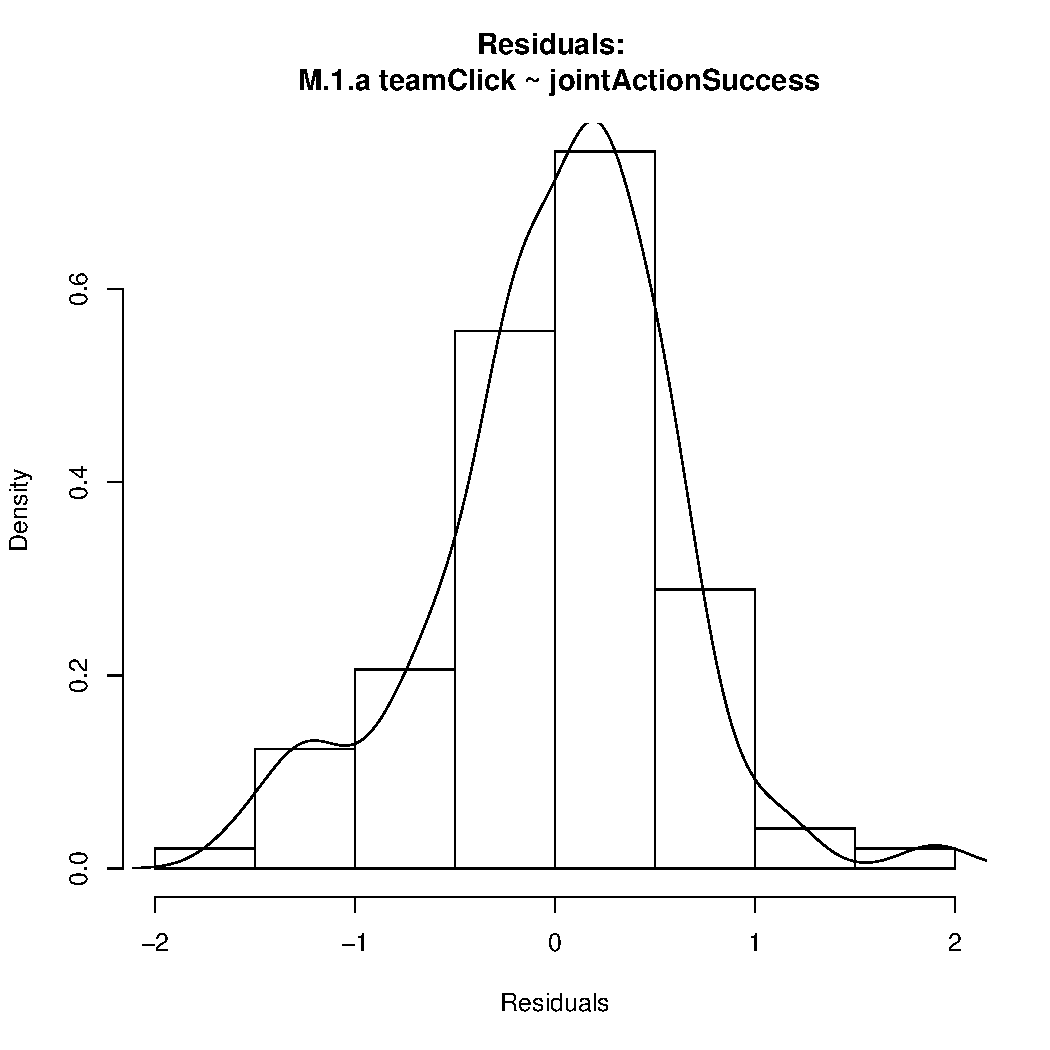
\includegraphics[scale =.4]{../images/MLM1aHist.pdf}
    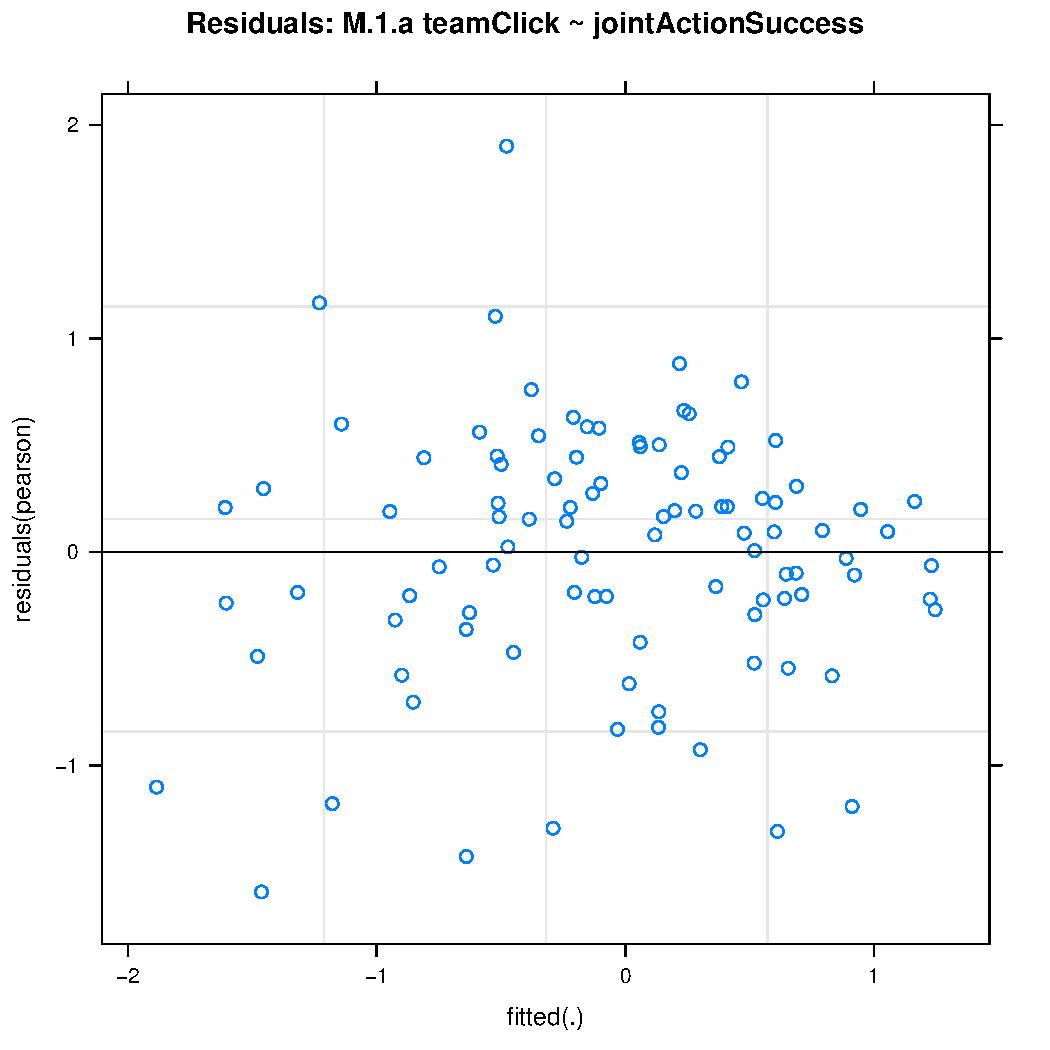
\includegraphics[scale =.4]{../images/MLM1aScatter.pdf}
    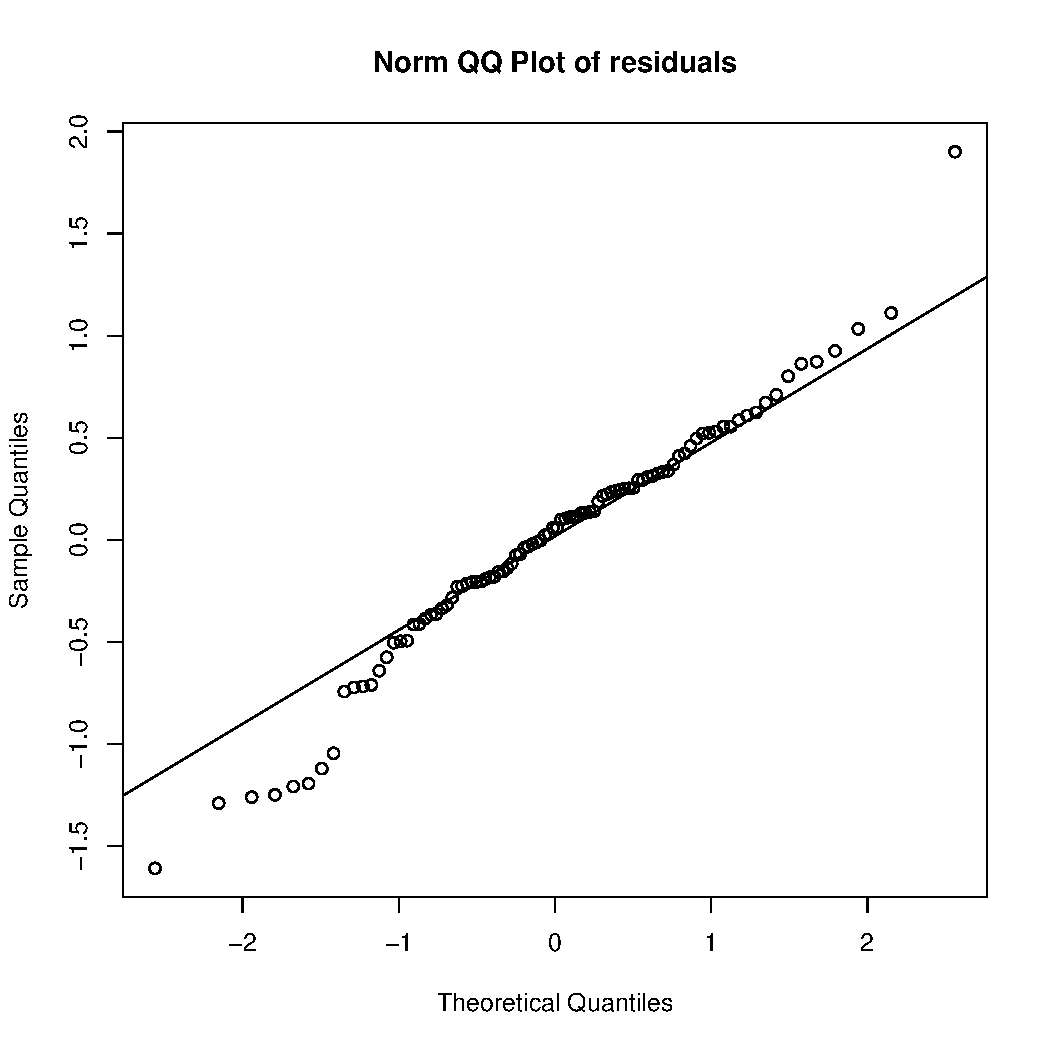
\includegraphics[scale =.4]{../images/MLM1aQQPlot.pdf}
    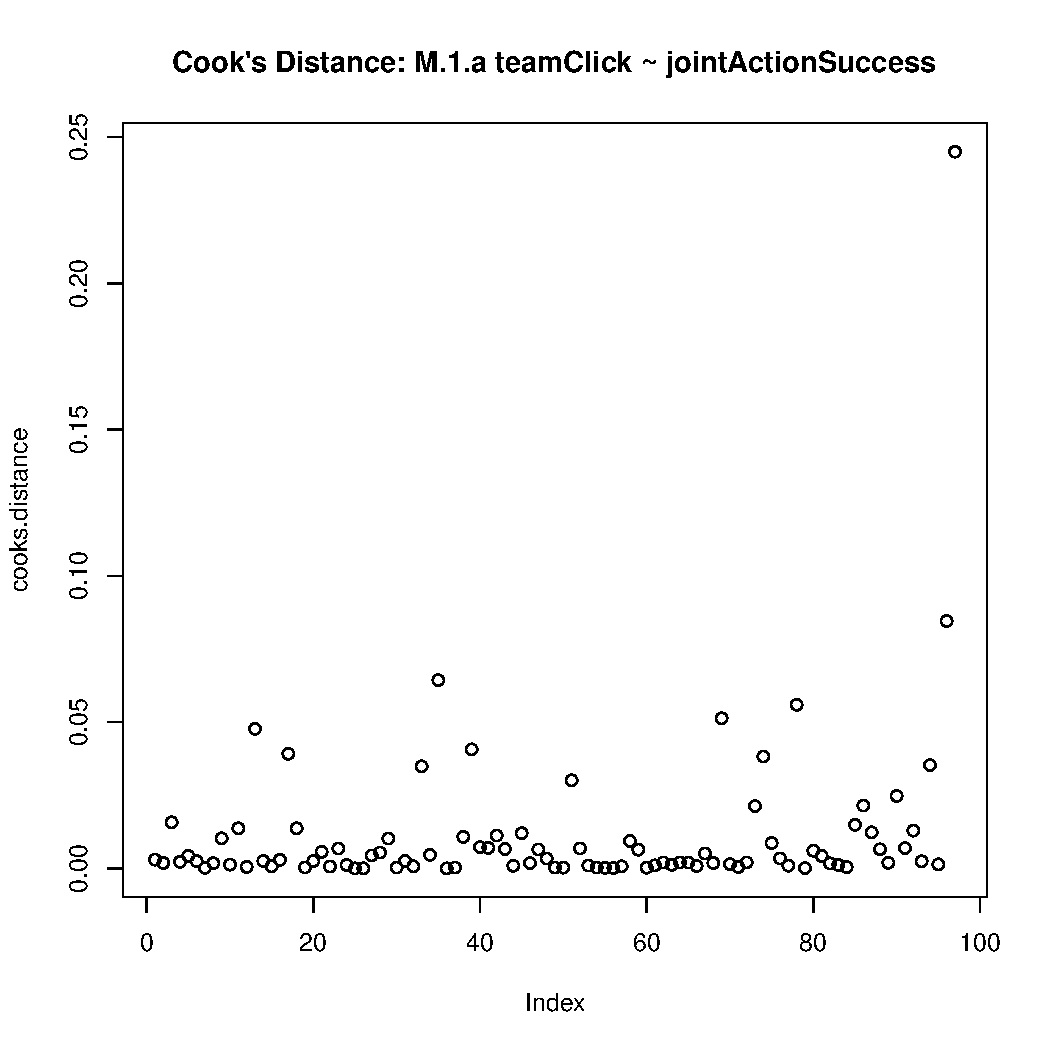
\includegraphics[scale =.4]{../images/MLM1aCooksD.pdf}
    \caption{Model Assumptions: 1.a Joint Action Success Predicts Team Click}
    \label{fig:MLM1aAssumptions}
\end{figure}



\subsubsection{1.b Team Performance Expectations predict Team Click}

To assess the prediction that more positive violations of expectations around team performance correlates with higher levels of team click, the following model was constructed:

\begin{equation}
  \begin{align*}
    Team Click =  & Team Performance Expectations \\
              &+ Individual Performance Expectations \\
              &+ Objective Competence + Subjective Competence \\
              &+ Tournament performance measures \\
  \end{align*}
\end{equation}

Expectations around individual performance, objective and subjective competence, and Tournament performance measures were introduced to the model as controls (fixed effects), while team was introduced as a random (level 2) effect.

Results of the model revealed a significant positive relationship between Team Performance Expectations and Team Click, $\beta = .02$ ($95\% CI =  0.01, 0.03$), $SE = 0.005$, $t(14.41) = 4.23$, $p < .001$, $marginal R^2 = .40$, $conditional R^2 = .56$. Expectations around individual performance ($\beta = .001$, $SE = .003$, $t(86.29) = .46$, $p = .65$), objective ($\beta = .01$, $SE = .09$, $t(84.94) = .13$, $p = .89$) and subjective competence ($\beta = .12$, $SE = .07$, $t(91) = 1.62$, $p = .11$), and Tournament performance measures  (final rank: $\beta = .08$, $SE = .05$, $t(44.33) = 1.72$, $p = .09$; total minutes: $\beta = .003$, $SE = .003$, $t(87.05) = 1.00$, $p = .32$); total points: $\beta = .001$, $SE = .005$, $t(84.94) = .21$, $p = .84$)) did not significantly predict team click.  The inclusion of these effects did, however, improve the model fit, as indicated by the reduced AIC and increased marginal $R^2$ value (see Table ~\ref{} for the various iterations of the model).  Model residuals were normally distributed around zero ($W = 0.98, p = .30$), and individual cases had low influence on the model (Cook's Distances all < .25, see Table ~\ref{fig:MLM1bAssumptions}).
%Need to account for very weak beta coefficient?



\begin{table}
\begin{center}
\begin{tabular}{l c c c }
\toprule
 & Intercept & Main effect & Controls \\
\midrule
(constant)                                 & $-0.04$  & $-0.00$               & $\mathbf{-0.79}^{*}$  \\
                                           & $(0.15)$ & $(0.09)$              & $(0.40)$              \\
Team Performance Vs Expectations           &          & $\mathbf{0.50}^{***}$ & $\mathbf{0.51}^{***}$ \\
                                           &          & $(0.11)$              & $(0.12)$              \\
Ind Performance Vs Expectations            &          &                       & $0.02$                \\
                                           &          &                       & $(0.08)$              \\
Objective Competence                       &          &                       & $0.02$                \\
                                           &          &                       & $(0.08)$              \\
Subjective Competence                      &          &                       & $0.12$                \\
                                           &          &                       & $(0.07)$              \\
Final Rank                                 &          &                       & $\mathbf{0.09}^{*}$   \\
                                           &          &                       & $(0.05)$              \\
Minutes Total                              &          &                       & $-0.00$               \\
                                           &          &                       & $(0.00)$              \\
Points Total                               &          &                       & $0.00$                \\
                                           &          &                       & $(0.01)$              \\
Fatigue                                    &          &                       & $\mathbf{0.18}^{*}$   \\
                                           &          &                       & $(0.09)$              \\
Extraverted                                &          &                       & $0.06$                \\
                                           &          &                       & $(0.05)$              \\
\midrule
AIC                                        & 299.06   & 268.43                & 228.63                \\
BIC                                        & 307.37   & 285.06                & 264.68                \\
Log Likelihood                             & -146.53  & -128.22               & -100.32               \\
Num. obs.                                  & 118      & 118                   & 97                    \\
Num. groups: team                          & 15       & 15                    & 14                    \\
\bottomrule
\multicolumn{4}{l}{\scriptsize{Coefficients with $p < 0.05$ in \textbf{bold}. Marginal $R^2 = .40$, Conditional $R^2 = .56$}}
\end{tabular}
\caption{Prediction 5: Team Performance Vs Expectations predicts Team Click in the Post-Tournament survey data (n = 97).}
\label{tab:MLM1bteamExpectationsClick}
\end{center}
\end{table}


\begin{figure}[htbp]
  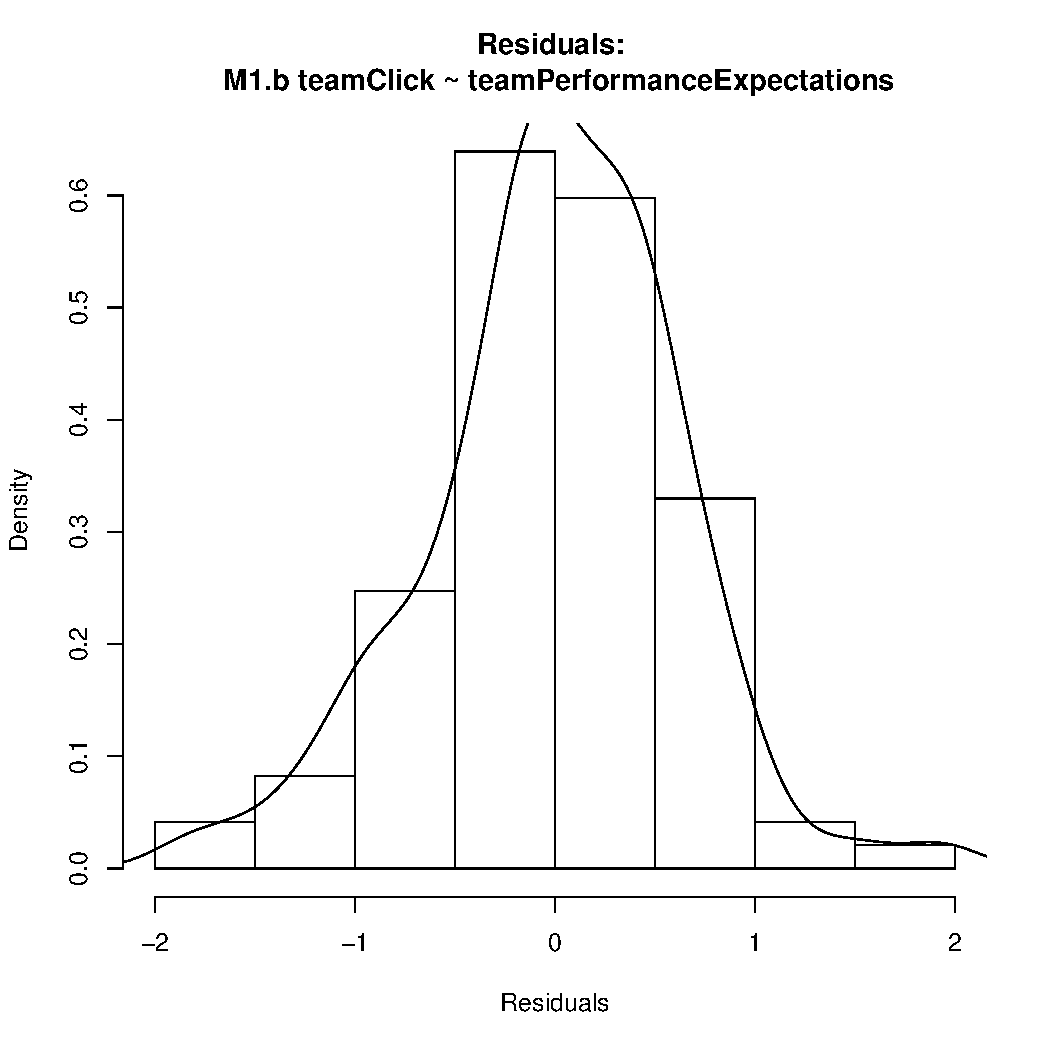
\includegraphics[scale =.4]{../images/MLM1bHist.pdf}
  \includegraphics[scale =.4]{../images/MLM1bScatter.pdf}
  \includegraphics[scale =.4]{../images/MLM1bQQNorm.pdf}
  \includegraphics[scale =.4]{../images/MLM1bCooksD.pdf}
  \caption{Model Assumptions: Model 1b Team Performance Expectations predict Team Click}
  \label{fig:MLM1bAssumptions}
\end{figure}








\subsubsection{1.c Team Performance Expectations moderates the effect of Joint Action Success on team Click}

If both perceptions of joint-action success and positive violations of expectations predicted team click, do these two predictors interact to predict click? Is team click higher for individuals whose perceived success in joint action was also a more positive violation of performance expectation? To test this possibility, the interaction term (Joint Action Success \times Team Performance Expectations) was included in model 1a as follows::

\begin{equation}
  \begin{align*}
    Team Click =  & Joint Action Success \times Team Performance Expectations \\
              &+ Individual Performance Success \\
              &+ Individual Performance Expectations \\
              &+ Objective Competence + Subjective Competence  \\
              &+ Tournament performance measures \\
  \end{align*}
\end{equation}
\bigskip
The inclusion of the interaction term failed to improve the model fit, judging by the relative goodness of fit, $AIC(1.c) = 217.91$ compared to $AIC(1.a) = 209.48$, $SD = .52 $, $\chi^2(18, N = 97) = 3.56$, $ p =.74$.  Results revealed that the interaction between Joint Action Success and Team Performance Expectations was not significant, $\beta < .001$ ($95\% CI =  -0.0062, 0.0063$), $SE = 0.005$, $t(14.41) = .026$, $p = .98$, $marginal R^2 = .56$, $conditional R^2 = .65$ (see Table ~\ref{tab:MLM1cPerformanceClickInteraction}).



% Table created by stargazer v.5.2 by Marek Hlavac, Harvard University. E-mail: hlavac at fas.harvard.edu
% Date and time: Mon, Jun 26, 2017 - 20:35:23
\begin{table}[!htbp] \centering 
  \caption{teamClick = jointActionSuccess X teamPerformanceExpectations} 
  \label{tab:MLM1cPerformanceClickInteraction} 
\footnotesize 
\begin{tabular}{@{\extracolsep{5pt}}lc} 
\\[-1.8ex]\hline 
\hline \\[-1.8ex] 
 & \multicolumn{1}{c}{\textit{Dependent variable:}} \\ 
\cline{2-2} 
\\[-1.8ex] & teamClick \\ 
\hline \\[-1.8ex] 
 (constant) & $-$0.83$^{*}$ \\ 
  & (0.41) \\ 
  & \\ 
 jointActionSuccess & 0.57$^{*}$ \\ 
  & (0.25) \\ 
  & \\ 
 teamPerformanceExpectations & 0.01 \\ 
  & (0.005) \\ 
  & \\ 
 indPerformanceSuccess & 0.01 \\ 
  & (0.10) \\ 
  & \\ 
 indPerformanceExpectations & $-$0.001 \\ 
  & (0.003) \\ 
  & \\ 
 objectiveCompetence & 0.06 \\ 
  & (0.08) \\ 
  & \\ 
 subjectiveCompetence & 0.10 \\ 
  & (0.07) \\ 
  & \\ 
 finalRank & 0.03 \\ 
  & (0.04) \\ 
  & \\ 
 minutesTotal & 0.01 \\ 
  & (0.003) \\ 
  & \\ 
 pointsTotal & 0.004 \\ 
  & (0.01) \\ 
  & \\ 
 teamPerformanceComponentsFactorPost:teamPerformance7 & 0.0001 \\ 
  & (0.003) \\ 
  & \\ 
\hline \\[-1.8ex] 
Marginal R-squared & .56 \\ 
Conditional R-squared & .65 \\ 
Observations & 97 \\ 
Log Likelihood & $-$90.96 \\ 
Akaike Inf. Crit. & 217.91 \\ 
Bayesian Inf. Crit. & 264.26 \\ 
\hline 
\hline \\[-1.8ex] 
\textit{Note:}  & \multicolumn{1}{r}{$^{*}$p$<$0.05; $^{**}$p$<$0.01; $^{***}$p$<$0.001} \\ 
\end{tabular} 
\end{table} 


%\textit{See appendix A for details about model assumptions}.
%\newpage
%\includegraphics[scale =.4]{../images/MLM1cHist.pdf}
%\includegraphics[scale =.4]{../images/MLM1cScatter.pdf}
%\includegraphics[scale =.4]{../images/MLM1cQQNorm.pdf}
%\includegraphics[scale =.4]{../images/MLM1cCooksD.pdf}

%\textit{problem here: increase in marginal and conditional R^2 values, perhaps due to adding additional variables into the model}
%The interaction did not improve the model fit,
%Nor did adding teamPerformance7 on its own into the model...
%But an interaction alone was significant

Findings from the first collection of models generally supported predictions. Team performance variables\nobreakdashperceptions of team component performance success and team performance relative to prior expectations\nobreakdashsignificantly predicted team click, when controlling for perceptions around individual performance (components and expectations), subjective and objective competence, and Tournament performance measures.  In addition, the relationship between violations of expectations around team performance and team click was also significant, such that more positive violations of expectations around team performance was associated with higher reported feelings of team click.  The interaction effect of joint-action success and team performance expectations violation on team click was not significant.  These three models provide evidence for the predictions that perceptions of joint-action success predicts team click among athletes in the Tournament.


\subsubsection{2.a Team Click predicts Social Bonding}

Next, the relationship between team click and social bonding was tested in the post-Tournament data. A linear mixed effects regression model was constructed with team as random effect, Team Click as fixed effect (predictor), and Social Bonding as outcome variable:

\begin{equation}
  \begin{align*}
    Social Bonding   =& Team Click\\
                    &+ Objective Competence + Subjective Competence  \\
                    &+ Tournament performance measures \\
  \end{align*}
\end{equation}
\bigskip

Controlling for Tournament performance measures and objective and subjective competence, the model revealed a significant relationship between team click and social bonding, $\beta = .67$ ($95\% CI =  .51, .84$), $SE = 0.08$, $t(16.01) = 8.22$, $p < .0001$, $marginal R^2 = .49$, $conditional R^2 = .51$ (see Table ~\ref{tab:MLM2aTeamClickBonding}).  Model residuals were normally distributed around zero ($W = 0.98, p = .15$), and individual cases had low influence on the model (Cook's Distances all < .15, see Figure ~\ref{fig:MKM2aAssumptions}).  This model supported the prediction that higher levels of team click would lead to higher levels of social bonding following intense exertive joint-activity.



% Table created by stargazer v.5.2 by Marek Hlavac, Harvard University. E-mail: hlavac at fas.harvard.edu
% Date and time: Mon, Jun 26, 2017 - 20:48:41
\begin{table}[!htbp] \centering 
  \caption{socialBonding = teamClick} 
  \label{tab:MLM2aTeamClickBonding} 
\begin{tabular}{@{\extracolsep{5pt}}lccc} 
\\[-1.8ex]\hline 
\hline \\[-1.8ex] 
 & \multicolumn{3}{c}{\textit{Dependent variable:}} \\ 
\cline{2-4} 
\\[-1.8ex] & \multicolumn{3}{c}{socialBonding} \\ 
\\[-1.8ex] & (1) & (2) & (3)\\ 
\hline \\[-1.8ex] 
 (constant) & $-$0.01 & $-$0.0002 & 0.21 \\ 
  & (0.10) & (0.07) & (0.27) \\ 
  & & & \\ 
 teamClick &  & 0.64$^{***}$ & 0.67$^{***}$ \\ 
  &  & (0.08) & (0.08) \\ 
  & & & \\ 
 objectiveCompetence &  &  & 0.04 \\ 
  &  &  & (0.08) \\ 
  & & & \\ 
 subjectiveCompetence &  &  & 0.12 \\ 
  &  &  & (0.07) \\ 
  & & & \\ 
 finalRank &  &  & $-$0.01 \\ 
  &  &  & (0.04) \\ 
  & & & \\ 
 minutesTotal &  &  & $-$0.003 \\ 
  &  &  & (0.004) \\ 
  & & & \\ 
 pointsTotal &  &  & $-$0.002 \\ 
  &  &  & (0.01) \\ 
  & & & \\ 
\hline \\[-1.8ex] 
Marginal R-squared &  &  & .49 \\ 
Conditional R-squared &  &  & .51 \\ 
Observations & 118 & 118 & 97 \\ 
Log Likelihood & $-$151.95 & $-$118.76 & $-$97.75 \\ 
Akaike Inf. Crit. & 309.90 & 249.53 & 217.50 \\ 
Bayesian Inf. Crit. & 318.21 & 266.15 & 245.82 \\ 
\hline 
\hline \\[-1.8ex] 
\textit{Note:}  & \multicolumn{3}{r}{$^{*}$p$<$0.05; $^{**}$p$<$0.01; $^{***}$p$<$0.001} \\ 
\end{tabular} 
\end{table} 


\begin{figure}[htbp]
  \includegraphics[scale =.4]{../images/MLM2aHist.pdf}
  \includegraphics[scale =.4]{../images/MLM2aScatter.pdf}
  \includegraphics[scale =.4]{../images/MLM2aQQNorm.pdf}
  \includegraphics[scale =.4]{../images/MLM2aCooksD.pdf}
  \caption{Model Assumptions: M2a Team Click predicts Social Bonding}
  \label{fig:MKM2aAssumptions}
\end{figure}









\subsubsection{3.a Joint Action Success predicts Social Bonding}

In light of evidence for significant relationships between joint-action success and team click, and team click and social bonding, the direct relationship between joint-action success and social bonding was assessed. Controlling for perceptions of success in individual performance, objective and subjective competence, and Tournament performance measures, the model revealed a significant effect of joint-action success on social bonding, $\beta = .45$ ($95\% CI =  .17, .73$), $SE = .14$, $t(23.4) = 3.19$, $p < .01$, $marginal R^2 = .27$, $conditional R^2 = .42$.  The model also revealed a significant positive effect of subjective measures of competence on social bonding, $\beta = .18$ ($95\% CI =  .03, .35$), $SE = .08$, $t(90.86) = 2.26$, $p = .03$ (full results in Table ~\ref{tab:MLM3aJointActionSuccessBonding}).

While Levene's Test for Equality of Variance indicated that the assumption of homoscedasticity was met at the group-level, $F(13,83) = .80, p = .66$, overall model residuals were non-normally distributed ($W = 0.95, p = .0007$), owing to relatively large negative skew (-.87) (see Figure ~\ref{fig:MLM3aAssumptions}). Non-normally distributed residuals are problematic as they may influence the model's ability to generate accurate parameter estimates . Two data manipulation techniques were considered in order to normalise residuals and therefore preserve the estimates of the model: exclusion of outliers and transformation of the outcome variable.  Transformation of the outcome variables was the preferred method over outlier exclusion, due to the cost involved in removing observations that may be of potential theoretical relevance to the scientific investigation \citep{Rousseeuw2011}. Nonetheless, for this first phase of analysis, both outlier exclusion and transformation manipulations of the data were performed and reported.

Exclusion of outliers according to Tukey's method (observations above and below 1.5 \times Inter Quartile Range (IQR), see \citep{Tukey1977}) appeared to improve the model fit, $\beta = .26$ ($95\% CI =  .05, .47$), $SE = 0.004$, $t(9.78) = 3.66$, $p < .01$, $marginal R^2 = .18$, $conditional R^2 = .34$.  The distribution of model residuals appeared to improve, but still violated the assumption of normality ($Shapiro-Wilk = 0.96, p = .009$).  Individual cases had low influence on the model (Cook's Distances all < .10).

Due to the \textit{positive} skew of the model residuals, the outcome variable was transformed by taking the log of the reversed scores of the outcome variable, i.e. $log10(k - y)$, where $k$ is a constant value from which each score for $y$ is subtracted so that the distribution of the outcome variable is reversed\citep{Howell2012}.\footnote{Reversing the distribution of the outcome variable allows the logarithmic function to normalise the distribution of the variable, by pushing them from the left hand side of the distribution towards the centre}  Transformed values were then returned to their original direction for analysis\citep{Field2012}.  Rebuilding the model with a log-transformed outcome variable appeared to improve the fit of the model more than the outlier-removed model, and came with the added bonus of not removing any observations. The distribution of residuals appeared more normal, ($W = 0.97, p = .04$), and the R-squared values for the model improved, $marginal R^2 = .27$, $conditional R^2 = .43$ (see Table ~\ref{tab:MLM3aJointActionSuccessBonding} for results of all three models, and Figures ~\ref{fig:MLM3aAssumptions}\nobreakdash~\ref{fig:MLM3aLogAssumptions} for tests for model assumptions).  Results of the log-transformed model indicated that the non-normally distributed residuals of the original model did not impact the estimates of the model. As such, the results of these models were taken as evidence for a significant positive relationship between perceptions of joint-action success and feelings of social bonding.


% Table created by stargazer v.5.2 by Marek Hlavac, Harvard University. E-mail: hlavac at fas.harvard.edu
% Date and time: Mon, Jun 26, 2017 - 21:18:41
\begin{table}[!htbp] \centering 
  \caption{socialBonding = jointActionSuccess} 
  \label{tab:MLM3aJointActionSuccessBonding} 
\footnotesize 
\begin{tabular}{@{\extracolsep{5pt}}lccc} 
\\[-1.8ex]\hline 
\hline \\[-1.8ex] 
 & \multicolumn{3}{c}{\textit{Dependent variable:}} \\ 
\cline{2-4} 
\\[-1.8ex] & socialBonding & bondingPostFactorOut & bondingPostFactorLogReturned \\ 
 &  & outliers removed & log-transformed \\ 
\\[-1.8ex] & (1) & (2) & (3)\\ 
\hline \\[-1.8ex] 
 (constant) & $-$0.06 & $-$0.06 & 1.97$^{***}$ \\ 
  & (0.31) & (0.31) & (0.13) \\ 
  & & & \\ 
 jointActionSuccess & 0.45$^{**}$ & 0.45$^{**}$ & 0.20$^{***}$ \\ 
  & (0.14) & (0.14) & (0.06) \\ 
  & & & \\ 
 indPerformanceSuccess & 0.05 & 0.05 & $-$0.001 \\ 
  & (0.11) & (0.11) & (0.05) \\ 
  & & & \\ 
 objectiveCompetence & 0.07 & 0.07 & 0.04 \\ 
  & (0.10) & (0.10) & (0.04) \\ 
  & & & \\ 
 subjectiveCompetence & 0.19$^{*}$ & 0.19$^{*}$ & 0.09$^{*}$ \\ 
  & (0.08) & (0.08) & (0.03) \\ 
  & & & \\ 
 finalRank & $-$0.02 & $-$0.02 & $-$0.01 \\ 
  & (0.05) & (0.05) & (0.02) \\ 
  & & & \\ 
 minutesTotal & 0.002 & 0.002 & 0.001 \\ 
  & (0.004) & (0.004) & (0.002) \\ 
  & & & \\ 
 pointsTotal & $-$0.001 & $-$0.001 & $-$0.002 \\ 
  & (0.01) & (0.01) & (0.003) \\ 
  & & & \\ 
\hline \\[-1.8ex] 
Marginal R-squared & .27 & .18 & .28 \\ 
Conditional R-squared & .42 & .34 & .43 \\ 
Observations & 97 & 97 & 97 \\ 
Log Likelihood & $-$113.05 & $-$113.05 & $-$29.49 \\ 
Akaike Inf. Crit. & 250.10 & 250.10 & 82.98 \\ 
Bayesian Inf. Crit. & 281.00 & 281.00 & 113.87 \\ 
\hline 
\hline \\[-1.8ex] 
\textit{Note:}  & \multicolumn{3}{r}{$^{*}$p$<$0.05; $^{**}$p$<$0.01; $^{***}$p$<$0.001} \\ 
\end{tabular} 
\end{table} 


\begin{figure}[htbp]
  \includegraphics[scale =.4]{../images/MLM3aHist.pdf}
  \includegraphics[scale =.4]{../images/MLM3aScatter.pdf}
  \includegraphics[scale =.4]{../images/MLM3aQQNorm.pdf}
  \includegraphics[scale =.4]{../images/MLM3aCooksD.pdf}
  \caption{Model Assumptions: M3a Joint Action Success predicts Social Bonding}
  \label{fig:MLM3aAssumptions}
\end{figure}

\begin{figure}[htbp]
  \includegraphics[scale =.4]{../images/MLM3aOutHist.pdf}
  \includegraphics[scale =.4]{../images/MLM3aOutScatter.pdf}
  \includegraphics[scale =.4]{../images/MLM3aOutQQNorm.pdf}
  \includegraphics[scale =.4]{../images/MLM3aOutCooksD.pdf}
  \caption{Model Assumptions: M3a Joint Action Success predicts Social Bonding (outliers removed)}
  \label{fig:MLM3aOutAssumptions}
\end{figure}

\begin{figure}[htbp]
  \includegraphics[scale =.4]{../images/MLM3aLogHist.pdf}
  \includegraphics[scale =.4]{../images/MLM3aLogScatter.pdf}
  \includegraphics[scale =.4]{../images/MLM3aLogQQNorm.pdf}
  \includegraphics[scale =.4]{../images/MLM3aLogCooksD.pdf}
  \caption{Model Assumptions: M3a Joint Action Success predicts Social Bonding (log-transformed)}
  \label{fig:MLM3aLogAssumptions}
\end{figure}








\subsubsection{3.b Team Performance Expectations -> Social Bonding} % very small effect

The direct relationship between expectations around team performance and social bonding was also tested.  The model revealed a significant positive relationship between Team Performance Expectations and Social Bonding, $\beta = .01$ ($95\% CI =  .002, .03$), $SE = .006$, $t(13.92) = 2.38$, $p = .03$, $marginal R^2 = .20$, $conditional R^2 = .40$.  The model also revealed a significant positive effect of Subjective Competence on Social Bonding, $\beta = .19$ ($95\% CI =  .002, .03$), $SE = .09$, $t(90.44) = 2.24$, $p = .03$.

Model residuals were not normally distributed, ($W = 0.91, p < .0001$), owing to large negative skew (-1.33) and high kurtosis  (2.49). Re-running the model with a log-transformed outcome variable appeared to make the best improvement to model residuals more than the outlier-removed model (see Table ~\ref{tab:MLM3bExpectationsBonding}). In the log-transformed model, the distribution of model residuals appeared most normal,  ($W = 0.97, p = .02$), and the R-squared values for the model improved, $marginal R^2 = .23$, $conditional R^2 = .44$.  Individual cases had low influence on the model (Cook's Distances all < .15, see Figures ~\ref{fig:MLM3bAssumptions} and ~\ref{fig:MLM3bLogAssumptions} for a comparison of model assumptions between the original and log-transformed model).

%Outlier exclusion
%Exclusion of outliers improved the distribution of residuals, ($W = 0.96, p = .007$), and individual cases had low influence on the model (Cook's Distances all < .15).  The significant positive effect of teamPerformanceExpectations on socialBonding remained in the adjusted model, $\beta = .01$ ($95\% CI =  .003, .02$), $SE = .004$, $t() = 2.65$, $p = .03$, $marginal R^2 = .19$, $conditional R^2 = .40$.  The effect of Subjective Competence on socialBonding was no longer significant, $\beta = .12$ ($95\% CI =  -.0004, .24$), $SE = .06$, $t(90.44) = 1.95$, $p = .06$.

\newgeometry{margin=0.5cm}

% Table created by stargazer v.5.2 by Marek Hlavac, Harvard University. E-mail: hlavac at fas.harvard.edu
% Date and time: Tue, Jun 27, 2017 - 17:01:54
\begin{table}[!htbp] \centering 
  \caption{M3.b socialBonding = teamPerformanceExpectations} 
  \label{tab:MLM3bExpectationsBonding} 
\scriptsize 
\begin{tabular}{@{\extracolsep{5pt}}lccc} 
\\[-1.8ex]\hline 
\hline \\[-1.8ex] 
 & \multicolumn{3}{c}{\textit{Dependent variable:}} \\ 
\cline{2-4} 
\\[-1.8ex] & socialBonding & bondingPostFactorOut & bondingPostFactorLogReturned \\ 
 &  & outliers removed & log-transformed \\ 
\\[-1.8ex] & (1) & (2) & (3)\\ 
\hline \\[-1.8ex] 
 (constant) & $-$1.67$^{*}$ & $-$1.18$^{*}$ & 1.19$^{***}$ \\ 
  & (0.73) & (0.53) & (0.31) \\ 
  & & & \\ 
 teamPerformanceExpectations & 0.01$^{*}$ & 0.01$^{**}$ & 0.01$^{**}$ \\ 
  & (0.01) & (0.004) & (0.003) \\ 
  & & & \\ 
 individualPerformanceExpectations & 0.004 & 0.001 & 0.001 \\ 
  & (0.004) & (0.003) & (0.002) \\ 
  & & & \\ 
 objectiveCompetence & 0.03 & 0.02 & 0.02 \\ 
  & (0.10) & (0.07) & (0.04) \\ 
  & & & \\ 
 subjectiveCompetence & 0.19$^{*}$ & 0.12 & 0.08$^{*}$ \\ 
  & (0.09) & (0.06) & (0.04) \\ 
  & & & \\ 
 finalRank & 0.08 & 0.10 & 0.04 \\ 
  & (0.13) & (0.09) & (0.05) \\ 
  & & & \\ 
 minutesTotal & 0.0003 & 0.001 & 0.0001 \\ 
  & (0.004) & (0.003) & (0.002) \\ 
  & & & \\ 
 pointsTotal & $-$0.04 & $-$0.06 & $-$0.03 \\ 
  & (0.09) & (0.06) & (0.04) \\ 
  & & & \\ 
 pointsTotal & $-$0.001 & $-$0.004 & $-$0.002 \\ 
  & (0.01) & (0.005) & (0.003) \\ 
  & & & \\ 
\hline \\[-1.8ex] 
Marginal R-squared & .20 & .19 & .23 \\ 
Conditional R-squared & .40 & .40 & .44 \\ 
Observations & 97 & 91 & 97 \\ 
Log Likelihood & $-$117.26 & $-$77.84 & $-$32.42 \\ 
Akaike Inf. Crit. & 260.52 & 181.67 & 90.85 \\ 
Bayesian Inf. Crit. & 293.99 & 214.31 & 124.32 \\ 
\hline 
\hline \\[-1.8ex] 
\textit{Note:}  & \multicolumn{3}{r}{$^{*}$p$<$0.05; $^{**}$p$<$0.01; $^{***}$p$<$0.001} \\ 
\end{tabular} 
\end{table} 

\restoregeometry

\begin{figure}[htbp]
  \includegraphics[scale =.4]{../images/MLM3bHist.pdf}
  \includegraphics[scale =.4]{../images/MLM3bScatter.pdf}
  \includegraphics[scale =.4]{../images/MLM3bQQNorm.pdf}
  \includegraphics[scale =.4]{../images/MLM3bCooksD.pdf}
  \caption{Model Assumptions: M3a Joint Action Success predicts Social Bonding (log-transformed)}
  \label{fig:MLM3bAssumptions}
\end{figure}

\begin{figure}[htbp]
  \includegraphics[scale =.4]{../images/MLM3bLogHist.pdf}
  \includegraphics[scale =.4]{../images/MLM3bLogScatter.pdf}
  \includegraphics[scale =.4]{../images/MLM3bLogQQNorm.pdf}
  \includegraphics[scale =.4]{../images/MLM3bLogCooksD.pdf}
  \caption{Model Assumptions: M3a Joint Action Success predicts Social Bonding (log-transformed)}
  \label{fig:MLM3bLogAssumptions}
\end{figure}





\subsubsection{Mediation analysis: Joint Action Success predicts Social Bonding, moderated by Team Click}

Results outlined above demonstrate significant relationships between joint-action success and team click, team click and social bonding, and a direct relationship between joint-action success and social bonding. Mediation analysis using linear mixed effects regressions in the Causal Mediation Analysis package in R (Version 4.4.5).  To make inferences concerning the average indirect and total effects, quasi-Bayesian Markov Chain Monte Carlo (MCMC) method based on normal approximation and 1000 simulations was used to estimate the 95\% Confidence Intervals \citep{Tofighi2016a,Imai2010}. MCMC estimation is a form of non-parametric bootstrapping whereby the sampling distribution for the effect of interest is not assumed to be normal but is instead simulated from the model estimates and their asymptotic variances and covariances \cite{Preacher2008}.

Results of the mediation analysis revealed significant average indirect effect of Joint Action Success on Social Bonding attributable to Team Click, $\beta = .37, 95\% CI = 0.20 , 0.59, p < .001$.  When controlling for the effect of team click on social bonding, the average direct effect between Joint Action Success and Social Bonding was no longer significant, $\beta = -.006, 95\% CI = -.27 , .23, p = .96 $ (see Figure ~\ref{}). The direct effect diminished such that including Joint Action Success in the model produced a total effect that was marginally \textit{smaller} than the indirect effect alone, $\beta = .36, 95\% CI = .13 , .61, p = .01$.  Residuals of the mediation model were normally distributed around zero, ($W = 0.99, p < .28$, see Figure ~\ref{fig:MLM4aAssumptions} for model assumptions).

These results suggest that feelings of team click fully mediate the relationship between perceptions of joint-action success and social bonding.

\begin{figure}[htbp]
  \centering
  \includegraphics[scale = .5]{../images/MLM4aMediationEffects.pdf}
  \caption{M4a Mediation Analysis}
  \label{fig:MLM4aMediationAnalysis}
\end{figure}

%\begin{figure}[htbp]
%  \includegraphics{finalDocuments/images/MLM4aResiduals.pdf}
%  \includegraphics{finalDocuments/images/MLM4aQQNorm.pdf}
%  \includegraphics{finalDocuments/images/MLM4aResiduals.pdf}
%  \includegraphics{finalDocuments/images/MLM4aCooksD.pdf}
%  \caption{M4a Mediation Analysis}
%  \label{fig:MLM4aAssumptions}
%\end{figure}

% (Baer et al 2006: 147) One method for constructing CIs assumes normality for the sampling distributions of the estimates. Under this assumption, 95% CIs for the average indirect effect and average total effect are obtained as Alternatively, one could perform a null hypothesis test by forming the critical ratio of each estimate to its standard error and comparing the result with the critical value of the z distribution. In andthe as- sumption of normality for the sampling distributions will not hold exactly, given that aˆb ˆ is a product of normally distributed estimates (and hence will not be normal). The deviation from normality may be small enough, however, that the CIs or significance tests will still be reasonably accurate.

%An alternative method for constructing CIs that may hold promise is the Monte Carlo (MC) method of MacKinnon et al. (2004). In this approach, the sampling distribution for the effect of interest is not assumed to be normal and is instead simulated from the model estimates and their asymptotic variances and covariances (a form of parametric bootstrap- ping). For instance, to simulate the sampling distribution of the average indirect effect, one would define a multinormal distribution with means equal to a ˆ, b ˆ, and ˆ aj ,bj and covariance matrix equal to the estimated covariance matrix of these estimates. One would then take random values from this multinormal distribution and plug them into Equation 5 to compute the average indirect effect. Collecting the results over many draws provides a simulated sampling distribution for the average indirect effect. One would then obtain conidence limits for the average indirect effect by taking the

%Preacher, K. J., & Selig, J. P. (2010, July). Monte Carlo method for assessing multilevel Mediation: An interactive tool for creating confidence intervals for indirect effects in 1-1-1 multilevel models [Computer software]. Available from http://quantpsy.org/.

\clearpage

\subsection{Summary of pre- to post-Tournament Results}





\subsubsection{$\Delta$Team Click $\sim$ $\Delta$Joint Action Success}

The first step was to test the prediction that a change in team click could be related to changes in athlete perception of joint-action success. Controlling for Tournament performance, measures and objective and subjective competence (fixed effects), and team-level variance (random effect), the model revealed a significant positive relationship between change in perceptions of joint-action success and change in feelings of team click, $\beta = .52$ ($95\% CI =  .34, .71$), $SE = 0.09$, $t(11.32) = 5.55$, $p < .001$, $marginal R^2 = .40$, $conditional R^2 = .47$ (see Table ~\ref{tab:MLM21aJointActionSuccesscClick} for results of all iterations of the model).  Model residuals were normally distributed around zero ($W = 0.98228, p = .22$), and individual cases had low influence on the model (Cook's Distances all < .20, see Figure \ref{fig:MLM21aAssumptions}).  This model supported the prediction that more positive perceptions of joint-action success correlate with stronger feelings of team click, by showing that athletes who experienced a positive increase in perceptions of joint-action success also reported a positive increase in feelings of team click throughout the Tournament.


% Table created by stargazer v.5.2 by Marek Hlavac, Harvard University. E-mail: hlavac at fas.harvard.edu
% Date and time: Tue, Jun 27, 2017 - 09:10:21
\begin{table}[!htbp] \centering 
  \caption{cTeamClick ~ cJointActionSuccess} 
  \label{tab:MLM21aJointActionSuccesscClick} 
\begin{tabular}{@{\extracolsep{5pt}}lccc} 
\\[-1.8ex]\hline 
\hline \\[-1.8ex] 
 & \multicolumn{3}{c}{\textit{Dependent variable:}} \\ 
\cline{2-4} 
\\[-1.8ex] & \multicolumn{3}{c}{cTeamClick} \\ 
\\[-1.8ex] & (1) & (2) & (3)\\ 
\hline \\[-1.8ex] 
 (constant) & 0.10 & 0.10 & $-$0.10 \\ 
  & (0.13) & (0.08) & (0.28) \\ 
  & & & \\ 
 cJointActionSuccess &  & 0.47$^{***}$ & 0.52$^{***}$ \\ 
  &  & (0.08) & (0.09) \\ 
  & & & \\ 
 cIndPerformanceSuccess &  &  & $-$0.04 \\ 
  &  &  & (0.09) \\ 
  & & & \\ 
 objectiveCompetence &  &  & 0.03 \\ 
  &  &  & (0.09) \\ 
  & & & \\ 
 subjectiveCompetence &  &  & $-$0.01 \\ 
  &  &  & (0.08) \\ 
  & & & \\ 
 finalRank &  &  & $-$0.02 \\ 
  &  &  & (0.04) \\ 
  & & & \\ 
 minutesTotal &  &  & 0.004 \\ 
  &  &  & (0.004) \\ 
  & & & \\ 
 pointsTotal &  &  & 0.01 \\ 
  &  &  & (0.01) \\ 
  & & & \\ 
\hline \\[-1.8ex] 
Marginal R-squared &  &  & .40 \\ 
Conditional R-squared &  &  & .47 \\ 
Observations & 99 & 99 & 97 \\ 
Log Likelihood & $-$130.59 & $-$107.75 & $-$104.44 \\ 
Akaike Inf. Crit. & 267.19 & 227.50 & 232.88 \\ 
Bayesian Inf. Crit. & 274.97 & 243.07 & 263.77 \\ 
\hline 
\hline \\[-1.8ex] 
\textit{Note:}  & \multicolumn{3}{r}{$^{*}$p$<$0.05; $^{**}$p$<$0.01; $^{***}$p$<$0.001} \\ 
\end{tabular} 
\end{table} 


\begin{figure}[htbp]
  \includegraphics[scale =.4]{../images/MLM21aHist.pdf}
  \includegraphics[scale =.4]{../images/MLM21aScatter.pdf}
  \includegraphics[scale =.4]{../images/MLM21aQQNorm.pdf}
  \includegraphics[scale =.4]{../images/MLM21aCooksD.pdf}
  \caption{Model Assumptions: M2.1a Change in Joint Action Success predicts change in Team Click}
  \label{fig:MLM21aAssumptions}
\end{figure}



\subsubsection{$\Delta$Team Click $\sim$ Team Performance Expectations}

Perception of team performance relative to prior expectations was substituted for change in perceptions of joint-action success to assess its relationship with team click. The model revealed a significant positive relationship between Team Performance Expectations and change in Team Click,  $\beta = .01$ ($95\% CI =  .002, .02$), $SE = 0.005$, $t(33.06) = 2.36$, $p = .02$, $marginal R^2 = .12$, $conditional R^2 = .22$, indicating that athletes who were more positive about their appraisals of team performance following the Tournament on average experienced an increase in feelings of team click. \\

Examination of model residuals revealed that they were not normally distributed around zero ($W = 0.95, p = .001$), due to positive skew (0.85) (see Figure ~\ref{fig:MLM21bAssumptions}).  Log-transformation of the outcome variable did not improve the non-normality of residuals, ($Shapiro-Wilk = 0.96, p = .008$).  Instead, exclusion of outliers according to Tukey's method appeared to improve the model fit,  improved the model fit such that residuals were normally distributed, ($Shapiro-Wilk = 0.99, p = .72$), and individual cases had low influence on the model (Cook's Distances all < .10, see Figure ~\ref{fig:MLM21bOutAssumptions}). The adjusted model supported the original significant positive effect of Team Performance Expectations on Team Click, $\beta = .02$ ($95\% CI =  .006, .02$), $SE = 0.004$, $t(9.78) = 3.66$, $p < .01$, $marginal R^2 = .17$, $conditional R^2 = .20$.  The adjusted model also revealed a significant negative effect of violations of expectations around individual performance on team click, $\beta = -.008 (95\% CI =  -.01, .001), SE = 0.004, t(91.79) = -2.28, p = .03$,  which could suggest that athletes who experienced more positive violations about their own performance did not feel the team click as strongly.  See Table ~\ref{tab:MLM21bOutLogComparison} for a comparison of adjusted models.


% Table created by stargazer v.5.2 by Marek Hlavac, Harvard University. E-mail: hlavac at fas.harvard.edu
% Date and time: Tue, Jun 27, 2017 - 09:21:13
\begin{table}[!htbp] \centering 
  \caption{M2.1b cTeamClick ~ cPerformanceExpectations} 
  \label{tab:MLM21bcTeamPerfExpcClick} 
\begin{tabular}{@{\extracolsep{5pt}}lccc} 
\\[-1.8ex]\hline 
\hline \\[-1.8ex] 
 & \multicolumn{3}{c}{\textit{Dependent variable:}} \\ 
\cline{2-4} 
\\[-1.8ex] & \multicolumn{3}{c}{cTeamClick} \\ 
\\[-1.8ex] & (1) & (2) & (3)\\ 
\hline \\[-1.8ex] 
 (constant) & 0.10 & $-$0.57 & $-$0.64 \\ 
  & (0.13) & (0.30) & (0.44) \\ 
  & & & \\ 
 cTeamPerformanceExpectations &  & 0.01$^{*}$ & 0.01$^{*}$ \\ 
  &  & (0.004) & (0.005) \\ 
  & & & \\ 
 cIndPerformanceExpectations &  &  & $-$0.003 \\ 
  &  &  & (0.004) \\ 
  & & & \\ 
 objectiveCompetence &  &  & $-$0.13 \\ 
  &  &  & (0.11) \\ 
  & & & \\ 
 subjectiveCompetence &  &  & $-$0.16 \\ 
  &  &  & (0.09) \\ 
  & & & \\ 
 finalRank &  &  & 0.02 \\ 
  &  &  & (0.06) \\ 
  & & & \\ 
 minutesTotal &  &  & 0.003 \\ 
  &  &  & (0.005) \\ 
  & & & \\ 
 pointsTotal &  &  & 0.003 \\ 
  &  &  & (0.01) \\ 
  & & & \\ 
\hline \\[-1.8ex] 
Marginal R-squared &  &  & .40 \\ 
Conditional R-squared &  &  & .47 \\ 
Observations & 99 & 99 & 97 \\ 
Log Likelihood & $-$130.59 & $-$127.00 & $-$123.15 \\ 
Akaike Inf. Crit. & 267.19 & 266.01 & 270.30 \\ 
Bayesian Inf. Crit. & 274.97 & 281.58 & 301.20 \\ 
\hline 
\hline \\[-1.8ex] 
\textit{Note:}  & \multicolumn{3}{r}{$^{*}$p$<$0.05; $^{**}$p$<$0.01; $^{***}$p$<$0.001} \\ 
\end{tabular} 
\end{table} 


\begin{table}
\begin{center}
\begin{tabular}{l c c c }
\toprule
 & Controls & Log-adjusted & Outliers removed \\
\midrule
(constant)                                 & $0.33$               & $\mathbf{1.27}^{***}$ & $0.40$                \\
                                           & $(0.51)$             & $(0.16)$              & $(0.39)$              \\
Team Performance Vs Expectations           & $\mathbf{0.30}^{**}$ & $\mathbf{0.09}^{*}$   & $\mathbf{0.32}^{***}$ \\
                                           & $(0.11)$             & $(0.04)$              & $(0.08)$              \\
Ind Performance Vs Expectations            & $-0.10$              & $-0.03$               & $\mathbf{-0.22}^{**}$ \\
                                           & $(0.10)$             & $(0.03)$              & $(0.08)$              \\
Objective Competence                       & $-0.15$              & $-0.05$               & $0.03$                \\
                                           & $(0.12)$             & $(0.04)$              & $(0.10)$              \\
Subjective Competence                      & $-0.15$              & $-0.05$               & $-0.03$               \\
                                           & $(0.09)$             & $(0.03)$              & $(0.08)$              \\
Final Rank                                 & $-0.01$              & $-0.00$               & $-0.08$               \\
                                           & $(0.06)$             & $(0.02)$              & $(0.04)$              \\
Minutes Total                              & $0.00$               & $0.00$                & $-0.00$               \\
                                           & $(0.01)$             & $(0.00)$              & $(0.00)$              \\
Points Total                               & $0.00$               & $0.00$                & $0.01$                \\
                                           & $(0.01)$             & $(0.00)$              & $(0.01)$              \\
Fatigue                                    & $-0.08$              & $-0.00$               & $-0.07$               \\
                                           & $(0.11)$             & $(0.04)$              & $(0.09)$              \\
Extraverted                                & $-0.06$              & $-0.02$               & $0.01$                \\
                                           & $(0.07)$             & $(0.02)$              & $(0.05)$              \\
\midrule
AIC                                        & 253.92               & 50.47                 & 200.30                \\
BIC                                        & 288.92               & 85.47                 & 234.66                \\
Log Likelihood                             & -112.96              & -11.23                & -86.15                \\
Num. obs.                                  & 90                   & 90                    & 86                    \\
Num. groups: team                          & 13                   & 13                    & 13                    \\

\bottomrule
\multicolumn{4}{l}{\scriptsize{Coefficients with $p < 0.05$ in \textbf{bold}. Effect size of model excluding outliers: Marginal $R^2 = .17$, Conditional $R^2 = .20$}}
\end{tabular}
\caption{Prediction 2: Team Click Change predicts Social Bonding Change in the Post-Tournament survey data (n = 90).}
\label{tab:MLM21bOutLogComparison}
\end{center}
\end{table}


\begin{figure}[htbp]
  \includegraphics[scale =.4]{../images/MLM21bHist.pdf}
  \includegraphics[scale =.4]{../images/MLM21bScatter.pdf}
  \includegraphics[scale =.4]{../images/MLM21bQQNorm.pdf}
  \includegraphics[scale =.4]{../images/MLM21bCooksD.pdf}
  \caption{Model Assumptions: M2.1b Team Performance Expectations post-Tournament predicts change in Team Click}
  \label{fig:MLM21bAssumptions}
\end{figure}


\begin{figure}[htbp]
  \includegraphics[scale =.4]{../images/MLM21bLogHist.pdf}
  \includegraphics[scale =.4]{../images/MLM21bLogScatter.pdf}
  \includegraphics[scale =.4]{../images/MLM21bLogQQNorm.pdf}
  \includegraphics[scale =.4]{../images/MLM21bLogCooksD.pdf}
  \caption{Model Assumptions: M2.1b Team Performance Expectations post-Tournament predicts change in Team Click (log-transformed)}
  \label{fig:MLM21bLogAssumptions}
\end{figure}


\begin{figure}[htbp]
  \includegraphics[scale =.4]{../images/MLM21bOutHist.pdf}
  \includegraphics[scale =.4]{../images/MLM21bOutScatter.pdf}
  \includegraphics[scale =.4]{../images/MLM21bOutQQNorm.pdf}
  \includegraphics[scale =.4]{../images/MLM21bOutCooksD.pdf}
  \caption{Model Assumptions: M2.1b Team Performance Expectations post-Tournament predicts change in Team Click (outliers removed)}
  \label{fig:MLM21bOutAssumptions}
\end{figure}

%Low values for both of these regression coefficients...


\subsubsection{$\Delta$Team Click $\sim$ $\Delta$Joint Action Success$\times$ Team Performance Expectations}

Introduction of the interaction effect of change in perceptions of joint-action success and expectations around team performance on Team Click was not significant, $\beta = .004$ ($95\% CI =  -.002, .01$), $SE = 0.003$, $t(30.14) = 1.42$, $p = .17$, $marginal R^2 = .40$, $conditional R^2 = .49$, and failed to improve the model fit, $\chi^2 = 2.72$, $ p = .44$ (see Table ~\ref{tab:MLM21ccTeamPerfExpcClickInt}).  This result indicates that the extent to which team performance violations were more or less positive did not have an additive effect on the positive relationship between perceptions of Joint Action Success and Team Click.



\subsubsection{$\Delta$Social Bonding$\sim$ $\Delta$Team Click}
Next, the change in social bonding observed pre- to post-Tournament was analysed as a function of change in feelings of team click. Controlling for Tournament performance and  objective and subjective competence (fixed), and team affiliation (random), the model revealed a significant positive effect of change in team click on change in social bonding, $\beta = .40$ ($95\% CI =  .16, .64$), $SE = .12$, $t(7.02) = 3.31$, $p = .01$, $marginal R^2 = .17$, $conditional R^2 = .23$ (see Table ~\ref{tab:MLM22acClickcBonding} for a full description of model estimates).  Model residuals were normally distributed around zero ($Shapiro-Wilk = 0.98, p = .15$). and individual cases had low influence on the model (Cook's Distances all < .6, see Figure ~\ref{fig:MLM22aAssumptions} for details). This model suggests that athletes who experienced an increase in feelings of team click also experienced an increase in feelings of social bonding towards their team.



\begin{table}
\begin{center}
\begin{tabular}{l c c c }
\toprule
 & Intercept & Main effect & Controls \\
\midrule
(constant)                                     & $\mathbf{0.34}^{***}$ & $\mathbf{0.31}^{***}$ & $0.29$               \\
                                               & $(0.09)$              & $(0.08)$              & $(0.46)$             \\
Team Click Change                              &                       & $\mathbf{0.39}^{***}$ & $\mathbf{0.37}^{**}$ \\
                                               &                       & $(0.11)$              & $(0.14)$             \\
Objective Competence                           &                       &                       & $0.08$               \\
                                               &                       &                       & $(0.10)$             \\
Subjective Competence                          &                       &                       & $0.01$               \\
                                               &                       &                       & $(0.09)$             \\
Final Rank                                     &                       &                       & $0.00$               \\
                                               &                       &                       & $(0.05)$             \\
Minutes Total                                  &                       &                       & $0.01$               \\
                                               &                       &                       & $(0.00)$             \\
Points Total                                   &                       &                       & $0.00$               \\
                                               &                       &                       & $(0.01)$             \\
Fatigue                                        &                       &                       & $-0.09$              \\
                                               &                       &                       & $(0.10)$             \\
Extraverted                                    &                       &                       & $-0.03$              \\
                                               &                       &                       & $(0.06)$             \\
\midrule
AIC                                            & 265.55                & 256.54                & 241.81               \\
BIC                                            & 273.34                & 272.11                & 274.31               \\
Log Likelihood                                 & -129.78               & -122.27               & -107.90              \\
Num. obs.                                      & 99                    & 99                    & 90                   \\
Num. groups: team                              & 14                    & 14                    & 13                   \\
\bottomrule
\multicolumn{4}{l}{\scriptsize{Coefficients with $p < 0.05$ in \textbf{bold}. Marginal $R^2 = .17$, Conditional $R^2 = .23$}}
\end{tabular}
\caption{Prediction 2: Team Click Change predicts Social Bonding Change in the Post-Tournament survey data (n = 90).}
\label{tab:MLM22acClickcBonding}
\end{center}
\end{table}


\begin{figure}[htbp]
  \includegraphics[scale =.4]{../images/MLM22aHist.pdf}
  \includegraphics[scale =.4]{../images/MLM22aScatter.pdf}
  \includegraphics[scale =.4]{../images/MLM22aQQNorm.pdf}
  \includegraphics[scale =.4]{../images/MLM22aCooksD.pdf}
  \caption{Model Assumptions: M2.2a Change in Team Click predicts change in Social Bonding}
  \label{fig:MLM22aAssumptions}
\end{figure}


%Exclusion of outliers according to Tukey's method (observations above and below 1.5 \times Inter Quartile Range (IQR)) appeared to improve the model fit, $\beta = .25$ ($95\% CI =  .11, .48$), $SE = .10$, $t(6.58) = 3.06$, $p < .02$, $marginal R^2 = .18$, $conditional R^2 = .25$. Model residuals were normally distributed, ($Shapiro-Wilk = 0.98, p = .14$),





\subsubsection{$\Delta$Social Bonding $\sim$ $\Delta$Joint Action Success}
Next, change in social bonding pre-post Tournament as a function of change in Joint Action Success was tested. Results of the model revealed a significant positive effect of change in Joint Action Success on changes in Social Bonding, $\beta = .38$ ($95\% CI =  .21, .56$), $SE = .09$, $t(97) = 4.35$, $p < .0001$, $marginal R^2 = .18$, $conditional R^2 = .18$, suggesting that on average, athletes who experienced an increase in positive perceptions of joint-action success as a result of the Tournament also experienced an increase in feelings of bondedness to their team.  Interestingly, the model also revealed a significant \textit{negative} effect of perceptions of success in individual component performance and social bonding, $\beta = -.23$ ($95\% CI =  -.44, -.02$), $SE = .11$, $t(97) = -2.12$, $p = .04$, indicating that athletes who were more positive about their own performance showed an average decrease in feelings of social bonding. All other fixed effects were not significant, see Table ~\ref{tab:MLM23acJointActionSuccesscBonding}. Model residuals were normally distributed around zero ($W = 0.98, p = .19$), and individual cases had low influence on the model (Cook's Distances all < .5, see Figure ~\ref{fig:MLM23aAssumptions}.



% Table created by stargazer v.5.2 by Marek Hlavac, Harvard University. E-mail: hlavac at fas.harvard.edu
% Date and time: Tue, Jun 27, 2017 - 17:13:12
\begin{table}[!htbp] \centering 
  \caption{cSocialBonding ~ cJointActionSuccess} 
  \label{tab:MLM23acJointActionSuccesscBonding} 
\footnotesize 
\begin{tabular}{@{\extracolsep{5pt}}lccc} 
\\[-1.8ex]\hline 
\hline \\[-1.8ex] 
 & \multicolumn{3}{c}{\textit{Dependent variable:}} \\ 
\cline{2-4} 
\\[-1.8ex] & \multicolumn{3}{c}{cSocialBonding} \\ 
\\[-1.8ex] & (1) & (2) & (3)\\ 
\hline \\[-1.8ex] 
 (constant) & 0.34$^{***}$ & 0.35$^{***}$ & 0.13 \\ 
  & (0.09) & (0.09) & (0.31) \\ 
  & & & \\ 
 cJointActionSuccess &  & 0.24$^{***}$ & 0.38$^{***}$ \\ 
  &  & (0.07) & (0.09) \\ 
  & & & \\ 
 cIndPerformanceSuccess &  &  & $-$0.23$^{*}$ \\ 
  &  &  & (0.11) \\ 
  & & & \\ 
 objectiveCompetence &  &  & 0.14 \\ 
  &  &  & (0.11) \\ 
  & & & \\ 
 subjectiveCompetence &  &  & 0.03 \\ 
  &  &  & (0.09) \\ 
  & & & \\ 
 finalRank &  &  & $-$0.04 \\ 
  &  &  & (0.05) \\ 
  & & & \\ 
 minutesTotal &  &  & 0.01 \\ 
  &  &  & (0.005) \\ 
  & & & \\ 
 pointsTotal &  &  & 0.003 \\ 
  &  &  & (0.01) \\ 
  & & & \\ 
\hline \\[-1.8ex] 
Marginal R-squared &  & .10 & .18 \\ 
Conditional R-squared &  & .10 & .18 \\ 
Observations & 99 & 99 & 97 \\ 
Log Likelihood & $-$129.78 & $-$124.37 & $-$118.30 \\ 
Akaike Inf. Crit. & 265.55 & 260.75 & 260.60 \\ 
Bayesian Inf. Crit. & 273.34 & 276.32 & 291.50 \\ 
\hline 
\hline \\[-1.8ex] 
\textit{Note:}  & \multicolumn{3}{r}{$^{*}$p$<$0.05; $^{**}$p$<$0.01; $^{***}$p$<$0.001} \\ 
\end{tabular} 
\end{table} 



\begin{figure}[htbp]
  \includegraphics[scale =.4]{../images/MLM23aHist.pdf}
  \includegraphics[scale =.4]{../images/MLM23aScatter.pdf}
  \includegraphics[scale =.4]{../images/MLM23aQQNorm.pdf}
  \includegraphics[scale =.4]{../images/MLM23aCooksD.pdf}
  \caption{Model Assumptions: M2.3a Change in Joint Action Success predicts change in Social Bonding}
  \label{fig:MLM23aAssumptions}
\end{figure}


\subsubsection{$\Delta$Social Bonding $\sim$ Team Performance Expectations}
A model designed to test the relationship between expectations around team performance and change in social bonding revealed a marginally significant main effect, $\beta = .008$ ($95\% CI =  -.0004, .02$), $SE = .004$, $t(97) = 1.87$, $p = .06$, $marginal R^2 = .05$, $conditional R^2 = .05$.  Examination of model residuals revealed that they were not normally distributed around zero ($Shapiro-Wilk = 0.96, p = .004$).  Re-running the model with a log-transformed outcome variable improved the model fit to the extent that residuals were near-normal, ($W= 0.97, p = .04$). When outliers were excluded from the model, the effect of Team Performance Expectations on Social Bonding was no longer significant, $\beta = .004$ ($95\% CI =  -.0004, .01$), $SE = .004$, $t(6.96) = 1.04$, $p = .33$, $marginal R^2 = .04$, $conditional R^2 = .20$ (see Table ~\ref{tab:MLM23bcBondingteamPerfExp} for full description of results).  These results from adjusted models suggests that variation in predictor variable did not suitably explain observed variation in the response.  As such, Team Performance Expectations was not considered in the subsequent mediation analysis.

\newgeometry{margin=0.5cm}

% Table created by stargazer v.5.2 by Marek Hlavac, Harvard University. E-mail: hlavac at fas.harvard.edu
% Date and time: Tue, Jun 27, 2017 - 17:15:15
\begin{table}[!htbp] \centering 
  \caption{cSocialBonding ~ teamPerformanceExpectations} 
  \label{tab:MLM23bcBondingteamPerfExp} 
\scriptsize 
\begin{tabular}{@{\extracolsep{5pt}}lccccc} 
\\[-1.8ex]\hline 
\hline \\[-1.8ex] 
 & \multicolumn{5}{c}{\textit{Dependent variable:}} \\ 
\cline{2-6} 
\\[-1.8ex] & \multicolumn{3}{c}{cSocialBonding} & bondingPostFactorLogReturned & bondingFactorChangePrePostOut \\ 
\\[-1.8ex] & (1) & (2) & (3) & (4) & (5)\\ 
\hline \\[-1.8ex] 
 (constant) & 0.34$^{***}$ & $-$0.07 & 0.01 & 1.34$^{***}$ & $-$0.01 \\ 
  & (0.09) & (0.25) & (0.39) & (0.22) & (0.33) \\ 
  & & & & & \\ 
 teamPerformanceExpectations &  & 0.01$^{*}$ & 0.01$^{*}$ & 0.01$^{***}$ & 0.005 \\ 
  &  & (0.004) & (0.004) & (0.003) & (0.004) \\ 
  & & & & & \\ 
 indPerformanceExpectations &  &  & $-$0.004 & 0.001 & $-$0.0000 \\ 
  &  &  & (0.004) & (0.002) & (0.003) \\ 
  & & & & & \\ 
 objectiveCompetence &  &  & 0.03 & 0.01 & 0.04 \\ 
  &  &  & (0.11) & (0.04) & (0.08) \\ 
  & & & & & \\ 
 subjectiveCompetence &  &  & $-$0.06 & 0.09$^{**}$ & $-$0.03 \\ 
  &  &  & (0.10) & (0.04) & (0.07) \\ 
  & & & & & \\ 
 finalRank &  &  & $-$0.03 & 0.01 & $-$0.03 \\ 
  &  &  & (0.05) & (0.02) & (0.04) \\ 
  & & & & & \\ 
 minutesTotal &  &  & 0.004 & 0.0003 & 0.001 \\ 
  &  &  & (0.005) & (0.002) & (0.003) \\ 
  & & & & & \\ 
 pointsTotal &  &  & 0.002 & $-$0.002 & $-$0.0003 \\ 
  &  &  & (0.01) & (0.003) & (0.01) \\ 
  & & & & & \\ 
\hline \\[-1.8ex] 
Marginal R-squared &  & .03 & .05 & .23 &  \\ 
Conditional R-squared &  & .03 & .05 & .46 &  \\ 
Observations & 99 & 99 & 97 & 97 & 86 \\ 
Log Likelihood & $-$129.78 & $-$128.30 & $-$125.20 & $-$32.67 & $-$75.13 \\ 
Akaike Inf. Crit. & 265.55 & 268.60 & 274.39 & 89.34 & 174.25 \\ 
Bayesian Inf. Crit. & 273.34 & 284.17 & 305.29 & 120.24 & 203.70 \\ 
\hline 
\hline \\[-1.8ex] 
\textit{Note:}  & \multicolumn{5}{r}{$^{*}$p$<$0.1; $^{**}$p$<$0.05; $^{***}$p$<$0.01} \\ 
\end{tabular} 
\end{table} 

% Table created by stargazer v.5.2 by Marek Hlavac, Harvard University. E-mail: hlavac at fas.harvard.edu
% Date and time: Tue, Jun 27, 2017 - 17:15:15
\begin{table}[!htbp] \centering 
  \caption{cSocialBonding ~ teamPerformanceExpectations} 
  \label{tab:MLM23bcBondingteamPerfExp} 
\scriptsize 
\begin{tabular}{@{\extracolsep{5pt}} ccc} 
\\[-1.8ex]\hline 
\hline \\[-1.8ex] 
$0.05$ & $0.01$ & $0.001$ \\ 
\hline \\[-1.8ex] 
\end{tabular} 
\end{table} 

\restoregeometry



\subsubsection{Mediation Analysis: $\Delta$Joint Action Success $\rightarrow$ $\Delta$Team Click $\rightarrow$ $\Delta$Social Bonding}

Results from the models reported above demonstrate significant relationships between 1) change in perceptions of joint-action success and changes in feelings of team click, 2) changes in feelings of team click and changes in feelings of social bonding, and a direct relationship between changes in joint-action success and changes in social bonding. A mediation analysis was performed to formally test whether a change in feelings of team click over the course of the Tournament mediated a direct relationship between change in perceptions of joint-action success and changes in perception of social bonding.\\

Results of the mediation analysis revealed that the average indirect effect of change in Joint Action Success on change in Social Bonding attributable to change in Team Click was not significant, $\beta = .14, 95\% CI = -.004 , .30, p = .06$, but was trending in the predicted direction (see Figure ~\ref{fig:MLM24aMediationAnalysis}).  When controlling for the effect of team click on social bonding, the average direct effect between Joint Action Success and Social Bonding was, however, significant, $\beta = .27, 95\% CI = .07 , .48, p < .001$.  The total effect of the meditation was also significant, $\beta = .41, 95\% CI = .21 , .63, p < .001$.  These results suggest a marginally-significant partial mediation effect of team click on the relationship between joint-action success and social bonding.  While the indirect effect of joint-action success on social bonding (mediated by team-click) was only marginally significant, this result does provide some support for the indirect effect observed in the post-Tournament data.  Considering the relatively small variation in change in team-click pre-post Tournament, to observe a marginally significant indirect effect of joint-action success on social bonding (mediated by team-click) in the pre-post-Tournament data is notable.


\begin{figure}[htbp]
  \centering
  \includegraphics[width=\columnwidth]{../images/MLM24aMediationAnalysis.pdf}
  \caption{M24a Mediation Analysis}
  \label{fig:MLM24aMediationAnalysis}
\end{figure}



\subsubsection{Additional Analysis: What predicts change in fusion to family?}
Both verbal and pictorial measures of fusion to team did not vary significantly in pre-post Tournament measures (see descriptives Table ~\ref{tab:factorsPrePostSummary}).  Interestingly, the pictorial measure of fusion, whose target was family, did increase significantly.  Exploratory analysis was performed to investigate the possible correlates of this increase. In line with the predictions of this study, we tested whether 1) changes in perceptions of Joint Action Success, 2) Team Click, and 3) their interaction (Joint Action Success x Team Click) predicted change in fusion to family.

\myparagraph{$\Delta$fusionFamily $\sim$ $\Delta$Joint Action Success}
The first model revealed a significant effect of change in perceptions of joint-action success and change in fusion to family, $\beta = .43$ ($95\% CI =  .07, .79$), $SE = .18$, $t(6.96) = 2.34$, $p = .$, $marginal R^2 = .11$, $conditional R^2 = .14$.  Model residuals indicated a poor model fit, ($W = 0.90$, $p < .00001$), due to high kurtosis ($> 2$), but not skew (.30). Given that log-transformation was not appropriate for normalising kurtosis (source), the analysis was re-run after excluding influential outliers.  The adjusted model was a much better fit, with model residuals normally distributed around zero, ($W = 0.99$, $p-value < .60$), see Table ~\ref{tab:MLM25acFusioncJointAction}. The model confirmed a significant positive relationship between change in perceptions of joint-action success and change in fusion to family, $\beta = .36$ ($95\% CI =  .19, .52$), $SE = .08$, $t() = 4.36$, $p = .$, $marginal R^2 = .32$, $conditional R^2 = .32$.


% Table created by stargazer v.5.2 by Marek Hlavac, Harvard University. E-mail: hlavac at fas.harvard.edu
% Date and time: Tue, Jun 27, 2017 - 10:42:15
\begin{table}[!htbp] \centering 
  \caption{cFusionFamily ~ jointActionSuccess} 
  \label{tab:MLM25acFusioncJointAction} 
\footnotesize 
\begin{tabular}{@{\extracolsep{5pt}}lcc} 
\\[-1.8ex]\hline 
\hline \\[-1.8ex] 
 & \multicolumn{2}{c}{\textit{Dependent variable:}} \\ 
\cline{2-3} 
\\[-1.8ex] & cFusionFamily & fusionPictorialFamilyChangeOut \\ 
 &  & outliers removed \\ 
\\[-1.8ex] & (1) & (2)\\ 
\hline \\[-1.8ex] 
 (constant) & 0.12 & $-$0.04 \\ 
  & (0.66) & (0.32) \\ 
  & & \\ 
 cJointActionSuccess & 0.43$^{**}$ & 0.50$^{***}$ \\ 
  & (0.18) & (0.10) \\ 
  & & \\ 
 cIndPerformanceSuccess & $-$0.46$^{**}$ & $-$0.01 \\ 
  & (0.20) & (0.10) \\ 
  & & \\ 
 teamPerformanceExpectations & $-$0.01 & 0.002 \\ 
  & (0.01) & (0.004) \\ 
  & & \\ 
 indPerformanceExpectations & 0.001 & $-$0.003 \\ 
  & (0.01) & (0.004) \\ 
  & & \\ 
 objectiveCompetence & 0.27 & 0.06 \\ 
  & (0.19) & (0.09) \\ 
  & & \\ 
 subjectiveCompetence & 0.06 & $-$0.0003 \\ 
  & (0.16) & (0.08) \\ 
  & & \\ 
 finalRank & 0.10 & $-$0.02 \\ 
  & (0.08) & (0.04) \\ 
  & & \\ 
 minutesTotal & $-$0.002 & 0.01 \\ 
  & (0.01) & (0.004) \\ 
  & & \\ 
\hline \\[-1.8ex] 
Marginal R-squared & .11 & .32 \\ 
Conditional R-squared & .14 & .32 \\ 
Observations & 97 & 97 \\ 
Log Likelihood & $-$173.00 & $-$104.99 \\ 
Akaike Inf. Crit. & 372.00 & 235.98 \\ 
Bayesian Inf. Crit. & 405.48 & 269.45 \\ 
\hline 
\hline \\[-1.8ex] 
\textit{Note:}  & \multicolumn{2}{r}{$^{*}$p$<$0.1; $^{**}$p$<$0.05; $^{***}$p$<$0.01} \\ 
\end{tabular} 
\end{table} 

% Table created by stargazer v.5.2 by Marek Hlavac, Harvard University. E-mail: hlavac at fas.harvard.edu
% Date and time: Tue, Jun 27, 2017 - 10:42:15
\begin{table}[!htbp] \centering 
  \caption{cFusionFamily ~ jointActionSuccess} 
  \label{tab:MLM25acFusioncJointAction} 
\footnotesize 
\begin{tabular}{@{\extracolsep{5pt}} ccc} 
\\[-1.8ex]\hline 
\hline \\[-1.8ex] 
$0.05$ & $0.01$ & $0.001$ \\ 
\hline \\[-1.8ex] 
\end{tabular} 
\end{table} 


%Need to do a multivariate regression here with family, country, team as outcomes?
\myparagraph{$\Delta$fusionFamily $\sim$ $\Delta$Team Click}

This model revealed that change in feelings of team-click was not a significant predictor of change in fusion to family, $\beta = .07$ ($95\% CI =  -.30, .44$), $SE = .19$, $t() = .38$, $p = .$, $marginal R^2 = .04$, $conditional R^2 = .07$. No other predictors in the model were statistically significant.

\myparagraph{$\Delta$fusionFamily $\sim$  $\Delta$Joint Action Success $\times$ $\Delta$Team Click}

The final model included an interaction between change in perceptions of joint-action success and change in feelings of team click as possible predictor of change in fusion to family.  Results of the model revealed that the interaction between change in perceptions of joint-action success and change in feelings of team-click was a significant positive predictor of change in fusion to family, $\beta = .22$ ($95\% CI =  .02, .41$), $SE = .10$, $t() = 2.22$, $p = .$, $marginal R^2 = .17$, $conditional R^2 = .23$. Model residuals were non-normally distributed, ($W = 0.93$, $p < .00001$).












%-------------------------------------------------------------------------------------%
%-------------------------------------------------------------------------------------%
%-------------------------------------------------------------------------------------%











\subsection{Overall Tournament Results}
In the final section, the entire data set was utilised to analyse a relationship between joint-action, team click, and social bonding. As described in the previous section, items relating to performance, team click, and social bonding that were consistent across the data set were reduced to factors in order to test study predictions. The repeated measures design of this analysis made it possible to statistically account for variation in responses due to repeated sampling of the same individual athlete throughout the Tournament, and due to the fact that each athlete was member of a specific team. The following models used a three-level structure, with responses across the four time points (level 1) nested within individual athletes (level 2), who were nested within individual teams (level 3). Both the slopes and intercepts were allowed to vary for every fixed effect of the model.


\subsubsection{Team Click $\sim$ Team Performance Expectations}

The first model tested the predicted relationship between joint-action and team click:
  \begin{equation}
    \begin{align*}
      Team Click =  & Team Performance Expectations  \\
                &+ Individual Performance Expectations   \\
                &+ Objective Competence + Subjective Competence \\
                &+ TournamentPerformanceMeasures  \\
    \end{align*}
  \end{equation}
  \bigskip

The model revealed a significant relationship between team performance expectation violation and team click, $\beta = .02$ ($95\% CI =  .019, .025$), $SE = .001$, $t(201) = 15.53$, $p < .0001$, $marginal R^2 = .65$, $conditional R^2 = .72$.  The model also indicated that individual performance expectation violation also significantly predicted team click, $\beta = .06$ ($95\% CI =  .001, .007$), $SE = .001$, $t(310) = 2.87$, $p < .01$, as did final rank in the Tournament, $\beta = .06$ ($95\% CI =  .04, .09$), $SE = .001$, $t(292) = 4.47$, $p < .0001$  (see Table ~\ref{tab:MLM31ateamPerfClickTournament} for full description of results).  The residuals of the model were normally distributed around zero, ($W = 0.99, p = .38$), and individual cases had low influence on the model (Cook's Distances all < .05) (see Figure ~\ref{fig:MLM31aTeamPerfExpClick}).  Results of the model suggest that, when controlling for individual performance, measures of objective and subjective competence, and Tournament performance, athletes whose expectations around team performance were more positively violated also experienced stronger feelings of team click.


\begin{table}
\begin{center}
\begin{tabular}{l c c c }
\toprule
 & Intercept & Main effect & Controls \\
\midrule
(constant)                                                        & $-0.00$  & $-0.06$               & $-0.12$               \\
                                                                  & $(0.04)$ & $(0.03)$              & $(0.21)$              \\
Team Performance Vs Expectations                                  &          & $\mathbf{0.74}^{***}$ & $\mathbf{0.72}^{***}$ \\
                                                                  &          & $(0.03)$              & $(0.05)$              \\
Ind Performance Vs Expectations                                   &          &                       & $\mathbf{0.12}^{**}$  \\
                                                                  &          &                       & $(0.04)$              \\
Objective Competence                                              &          &                       & $0.04$                \\
                                                                  &          &                       & $(0.04)$              \\
Subjective Competence                                             &          &                       & $0.07$                \\
                                                                  &          &                       & $(0.04)$              \\
Final Rank                                                        &          &                       & $-0.00$               \\
                                                                  &          &                       & $(0.02)$              \\
Minutes Total                                                     &          &                       & $-0.00$               \\
                                                                  &          &                       & $(0.00)$              \\
Points Total                                                      &          &                       & $0.00$                \\
                                                                  &          &                       & $(0.00)$              \\
Fatigue                                                           &          &                       & $0.00$                \\
                                                                  &          &                       & $(0.00)$              \\
Extraverted                                                       &          &                       & $0.01$                \\
                                                                  &          &                       & $(0.03)$              \\
\midrule
AIC                                                               & 1552.70  & 842.67                & 602.59                \\
BIC                                                               & 1570.04  & 879.53                & 665.89                \\
Log Likelihood                                                    & -772.35  & -412.33               & -284.30               \\
Num. obs.                                                         & 564      & 444                   & 306                   \\
\bottomrule
\multicolumn{4}{l}{\scriptsize{Coefficients with $p < 0.05$ in \textbf{bold}. Marginal $R^2 = .63$, Conditional $R^2 = .69$}}
\end{tabular}
\caption{Prediction 1: Team Performance Vs Expectations predicts Team Click in the Overall Tournament survey data (n = 90).}
\label{tab:MLM31ateamPerfClickTournament}
\end{center}
\end{table}


\begin{figure}[htbp]
  \includegraphics[scale =.4]{../images/MLM31aHist.pdf}
  \includegraphics[scale =.4]{../images/MLM31aScatter.pdf}
  \includegraphics[scale =.4]{../images/MLM31aQQNorm.pdf}
  \includegraphics[scale =.4]{../images/MLM31aCooksD.pdf}
  \caption{Model Assumptions: M3.1a Team Performance Expectations Predict Team Click}
  \label{fig:MLM31aTeamPerfExpClick}
\end{figure}



\subsubsection{Social Bonding $\sim$ Team Click}
The relationship between team click and social bonding was tested. Controlling for perceptions of individual performance, measures of objective and subjective competence, and Tournament performance, the model revealed a significant positive relationship between feelings of team click and feelings of social bonding, $\beta = .65$ ($95\% CI =  .56, .74$), $SE = .03$, $t(91) = 13.86$, $p < .0001$, $marginal R^2 = .49$, $conditional R^2 = .66$ (see Table ~\ref{tab:MLM31bclickBondingTournament} for complete description of model estimates). Model residuals were not normally distributed around zero, ($W = 0.92, p < .00001$), owing to high negative skew (-1.24) and high kurtosis (5.12) (see Figure ~\ref{fig:MLM31bAssumptions}). Both log transformation ($W = 0.95, p < .00001$) and outlier removal ($W = 0.96, p < .00001$) procedures improved the model fit marginally, but not within the bounds of normality. To resolve this assumption violation, the outcome variable was first subjected to outlier-removal, and then subsequently log-transformed, which appeared to improve the distribution of residuals somewhat, ($W = 0.98, p = .0002$, see Table ~\ref{MLM31bclickBondingTournamentModelComparison} for adjusted model comparisons and Figure ~\ref{fig:MLM31bLogOutAssumptions} for adjusted model residuals).  The adjusted model confirmed a significant positive effect of team click on social bonding over the course of the Tournament, $\beta = .15$ ($95\% CI =  .11, .19$), $SE = .02$, $t() = 8.38$, $p < .001$, $marginal R^2 = .23$, $conditional R^2 = .34$.  These results suggest that on average, athletes who experienced higher feelings of team click also experienced higher levels of social bonding throughout the course of the Tournament.



% Table created by stargazer v.5.2 by Marek Hlavac, Harvard University. E-mail: hlavac at fas.harvard.edu
% Date and time: Thu, Sep 14, 2017 - 09:39:55
\begin{table}[!htbp] \centering 
  \caption{bondingTournament ~ teamClickTournament} 
  \label{tab:MLM31bclickBondingTournament} 
\footnotesize 
\begin{tabular}{@{\extracolsep{5pt}}lccc} 
\\[-1.8ex]\hline 
\hline \\[-1.8ex] 
 & \multicolumn{3}{c}{\textit{Dependent variable:}} \\ 
\cline{2-4} 
\\[-1.8ex] & (1) & (2) & (3)\\ 
\hline \\[-1.8ex] 
 (constant) & $-$0.00 & $-$1.46$^{***}$ & $-$1.59$^{***}$ \\ 
  & (0.04) & (0.08) & (0.15) \\ 
  & & & \\ 
 teamPerformanceExpectations &  & 0.02$^{***}$ & 0.02$^{***}$ \\ 
  &  & (0.001) & (0.001) \\ 
  & & & \\ 
 indPerformanceExpectations &  &  & 0.004$^{**}$ \\ 
  &  &  & (0.002) \\ 
  & & & \\ 
 objectiveCompetence &  &  & 0.02 \\ 
  &  &  & (0.04) \\ 
  & & & \\ 
 subjectiveCompetence &  &  & 0.08$^{*}$ \\ 
  &  &  & (0.04) \\ 
  & & & \\ 
 finalRank &  &  & $-$0.0002 \\ 
  &  &  & (0.02) \\ 
  & & & \\ 
 minutesTotal &  &  & $-$0.001 \\ 
  &  &  & (0.002) \\ 
  & & & \\ 
 pointsTotal &  &  & 0.003 \\ 
  &  &  & (0.003) \\ 
  & & & \\ 
\hline \\[-1.8ex] 
Marginal R-squared & .47 & .49 &  \\ 
Conditional R-squared & .66 & .66 &  \\ 
Observations & 564 & 444 & 331 \\ 
Log Likelihood & $-$772.35 & $-$412.33 & $-$303.82 \\ 
Akaike Inf. Crit. & 1,552.70 & 842.67 & 637.65 \\ 
Bayesian Inf. Crit. & 1,570.04 & 879.53 & 694.68 \\ 
\hline 
\hline \\[-1.8ex] 
\textit{Note:}  & \multicolumn{3}{r}{$^{*}$p$<$0.05; $^{**}$p$<$0.01; $^{***}$p$<$0.001} \\ 
\end{tabular} 
\end{table} 



% Table created by stargazer v.5.2 by Marek Hlavac, Harvard University. E-mail: hlavac at fas.harvard.edu
% Date and time: Thu, Sep 14, 2017 - 09:39:58
\begin{table}[!htbp] \centering 
  \caption{Model Adjustment Comparison:bondingTournament ~ teamClickTournament} 
  \label{MLM31bclickBondingTournamentModelComparison} 
\tiny 
\begin{tabular}{@{\extracolsep{5pt}}lcccc} 
\\[-1.8ex]\hline 
\hline \\[-1.8ex] 
 & \multicolumn{4}{c}{\textit{Dependent variable:}} \\ 
\cline{2-5} 
 & model & log-transformed & outliers removed & outliers + log-transformed \\ 
\\[-1.8ex] & (1) & (2) & (3) & (4)\\ 
\hline \\[-1.8ex] 
 (constant) & $-$1.59$^{***}$ & 1.63$^{***}$ & 0.31$^{***}$ & 1.50$^{***}$ \\ 
  & (0.15) & (0.02) & (0.08) & (0.04) \\ 
  & & & & \\ 
 teamPerformanceExpectations & 0.02$^{***}$ &  &  &  \\ 
  & (0.001) &  &  &  \\ 
  & & & & \\ 
 indPerformanceExpectations & 0.004$^{**}$ &  &  &  \\ 
  & (0.002) &  &  &  \\ 
  & & & & \\ 
 objectiveCompetence &  & 0.16$^{***}$ & 0.42$^{***}$ & 0.19$^{***}$ \\ 
  &  & (0.01) & (0.04) & (0.02) \\ 
  & & & & \\ 
 subjectiveCompetence & 0.02 & 0.01 & 0.01 & 0.01 \\ 
  & (0.04) & (0.01) & (0.03) & (0.01) \\ 
  & & & & \\ 
 finalRank & 0.08$^{*}$ & 0.01 & 0.03 & 0.02 \\ 
  & (0.04) & (0.01) & (0.02) & (0.01) \\ 
  & & & & \\ 
 minutesTotal & $-$0.0002 & $-$0.004 & $-$0.01 & $-$0.01 \\ 
  & (0.02) & (0.003) & (0.01) & (0.005) \\ 
  & & & & \\ 
 pointsTotal & $-$0.001 & $-$0.001 & $-$0.002 & $-$0.001 \\ 
  & (0.002) & (0.0004) & (0.001) & (0.001) \\ 
  & & & & \\ 
 pointsTotal & 0.003 & $-$0.001 & $-$0.001 & $-$0.001 \\ 
  & (0.003) & (0.001) & (0.002) & (0.001) \\ 
  & & & & \\ 
\hline \\[-1.8ex] 
Marginal R-squared & .49 & .50 & .23 & .23 \\ 
Conditional R-squared & .66 & .61 & .35 & .34 \\ 
Shapiro-Wilk Test (p-value) & .92(<.00000000001) & .95(<.000001) & .96(<.00001) & .98(.0002) \\ 
Observations & 331 & 449 & 405 & 405 \\ 
Log Likelihood & $-$303.82 & 225.59 & $-$241.97 & 79.71 \\ 
Akaike Inf. Crit. & 637.65 & $-$423.18 & 511.94 & $-$131.42 \\ 
Bayesian Inf. Crit. & 694.68 & $-$365.69 & 567.99 & $-$75.37 \\ 
\hline 
\hline \\[-1.8ex] 
\textit{Note:}  & \multicolumn{4}{r}{$^{*}$p$<$0.05; $^{**}$p$<$0.01; $^{***}$p$<$0.001} \\ 
\end{tabular} 
\end{table} 



\begin{figure}[htbp]
  \includegraphics[scale =.4]{../images/MLM31bHist.pdf}
  \includegraphics[scale =.4]{../images/MLM31bScatter.pdf}
  \includegraphics[scale =.4]{../images/MLM31bQQNorm.pdf}
  \includegraphics[scale =.4]{../images/MLM31bCooksD.pdf}
  \caption{Model Assumptions: M3.1b Team Click Predict Social Bonding}
  \label{fig:MLM31bAssumptions}
\end{figure}


\begin{figure}[htbp]
  \includegraphics[scale =.4]{../images/MLM31bOutLogHist.pdf}
  \includegraphics[scale =.4]{../images/MLM31bOutLogScatter.pdf}
  \includegraphics[scale =.4]{../images/MLM31bOutLogQQNorm.pdf}
  \includegraphics[scale =.4]{../images/MLM31bOutLogCooksD.pdf}
  \caption{Model Assumptions: M3.1b Team Click predicts Social Bonding (log/outlier adjusted)}
  \label{fig:MLM31bLogOutAssumptions}
\end{figure}






\subsubsection{Social Bonding $\sim$ Team Performance Expectations}
Next, the direct relationship between Team Performance Expectations and social bonding was tested.  The model revealed a significant positive relationship between team performance expectation violation and social bonding, $\beta = .01$ ($95\% CI =  .009, .02$), $SE = .002$, $t() = 6.66$, $p < .001$, $marginal R^2 = .33$, $conditional R^2 = .53$ (see Table ~\ref{tab:MLM32ateamPerfBondingTournament} for full description of model estimates).  \\

Model residuals were non-normally distributed, ($W = 0.97, p < .00001$), with negative skew ($-.6$), and higher than normal kurtosis, see Figure ~\ref{fig:MLM32aAssumptions}.  A model in which the outcome was log-transformed following removal of outliers provided the best possible fit for the available data ~\ref{MLM32ateamPerfBondingTournamentModelComparison}. While the distribution of errors was still non-normal, ($W = 0.97, p < .00001$),  error terms appear much more evenly distributed around zero than the original model . The adjusted model confirmed the significant positive effect of team performance expectation violation on social bonding,  $\beta = .003$ ($95\% CI =  .0009, .02$), $SE = .003$, $t() = 3.67$, $p < .001$, $marginal R^2 = .09$, $conditional R^2 = .17$.



\begin{table}
\begin{center}
\begin{tabular}{l c c c c }
\toprule
 & Main effect & Controls & Log-transformed & Log and outliers \\
\midrule
(constant)                        & $-0.00$               & $\mathbf{0.51}^{*}$   & $\mathbf{1.71}^{***}$ & $\mathbf{1.64}^{***}$ \\
                                  & $(0.04)$              & $(0.26)$              & $(0.06)$              & $(0.08)$              \\
Team Performance Vs Expectations  & $\mathbf{0.59}^{***}$ & $\mathbf{0.47}^{***}$ & $\mathbf{0.11}^{***}$ & $\mathbf{0.07}^{***}$ \\
                                  & $(0.04)$              & $(0.06)$              & $(0.01)$              & $(0.02)$              \\
Ind Performance Vs Expectations   &                       & $\mathbf{0.25}^{***}$ & $\mathbf{0.05}^{***}$ & $0.01$                \\
                                  &                       & $(0.06)$              & $(0.01)$              & $(0.02)$              \\
Objective Competence              &                       & $0.07$                & $0.02$                & $0.01$                \\
                                  &                       & $(0.05)$              & $(0.01)$              & $(0.02)$              \\
Subjective Competence             &                       & $0.09$                & $\mathbf{0.02}^{*}$   & $\mathbf{0.03}^{*}$   \\
                                  &                       & $(0.05)$              & $(0.01)$              & $(0.01)$              \\
Final Rank                        &                       & $-0.03$               & $-0.01$               & $-0.01$               \\
                                  &                       & $(0.02)$              & $(0.01)$              & $(0.01)$              \\
Minutes Total                   &                       & $-0.01$  & $-0.00$  & $-0.00$               \\
                                  &                       & $(0.00)$              & $(0.00)$              & $(0.00)$              \\
Points Total                      &                       & $0.00$                & $0.00$                & $0.00$                \\
                                  &                       & $(0.00)$              & $(0.00)$              & $(0.00)$              \\
Fatigue                           &                       & $0.00$                & $0.00$                & $0.00$                \\
                                  &                       & $(0.00)$              & $(0.00)$              & $(0.00)$              \\
Extraverted                       &                       & $-0.04$               & $-0.01$               & $-0.02$               \\
                                  &                       & $(0.03)$              & $(0.01)$              & $(0.01)$              \\
\midrule
AIC                               & 1083.79               & 752.42                & -131.94               & -8.28                 \\
BIC                               & 1104.27               & 800.83                & -83.53                & 38.54                 \\
Log Likelihood                    & -536.89               & -363.21               & 78.97                 & 17.14                 \\
Num. obs.                         & 444                   & 306                   & 306                   & 271                   \\
\bottomrule
\multicolumn{5}{l}{\scriptsize{Coefficients with $p < 0.05$ in \textbf{bold}. Effect sizes of the Log and outlier model: Marginal $R^2 = .36$, Conditional $R^2 = .36$}}
\end{tabular}
\caption{Prediction 3: Team Performance Vs Expectations predicts Social Bonding in the Overall Tournament survey data (n = 90).}
\label{tab:MLM32ateamPerfBondingTournament}
\end{center}
\end{table}



% Table created by stargazer v.5.2 by Marek Hlavac, Harvard University. E-mail: hlavac at fas.harvard.edu
% Date and time: Thu, Sep 14, 2017 - 09:42:11
\begin{table}[!htbp] \centering 
  \caption{Model Comparison: M3.2a socialBondingTournament ~ teamPerformanceExpectationsTournament} 
  \label{tab:MLM32ateamPerfBondingTournamentModelComparison} 
\scriptsize 
\begin{tabular}{@{\extracolsep{5pt}}lccc} 
\\[-1.8ex]\hline 
\hline \\[-1.8ex] 
 & \multicolumn{3}{c}{\textit{Dependent variable:}} \\ 
\cline{2-4} 
 & model & log-transformed & outliers+log-transformed \\ 
\\[-1.8ex] & (1) & (2) & (3)\\ 
\hline \\[-1.8ex] 
 (constant) & $-$0.70$^{***}$ & 1.42$^{***}$ & 1.42$^{***}$ \\ 
  & (0.18) & (0.04) & (0.06) \\ 
  & & & \\ 
 teamPerformanceExpectations & 0.01$^{***}$ & 0.003$^{***}$ & 0.003$^{***}$ \\ 
  & (0.002) & (0.0005) & (0.001) \\ 
  & & & \\ 
 indPerformanceExpectations & 0.01$^{**}$ & 0.001$^{**}$ & 0.0001 \\ 
  & (0.002) & (0.0004) & (0.001) \\ 
  & & & \\ 
 objectiveCompetence & 0.04 & 0.01 & 0.01 \\ 
  & (0.05) & (0.01) & (0.02) \\ 
  & & & \\ 
 subjectiveCompetence & 0.10$^{*}$ & 0.03$^{*}$ & 0.03$^{*}$ \\ 
  & (0.04) & (0.01) & (0.01) \\ 
  & & & \\ 
 finalRank & $-$0.04 & $-$0.01 & $-$0.01 \\ 
  & (0.02) & (0.005) & (0.01) \\ 
  & & & \\ 
 minutesTotal & $-$0.003 & $-$0.001 & $-$0.001 \\ 
  & (0.002) & (0.001) & (0.001) \\ 
  & & & \\ 
 pointsTotal & 0.001 & 0.0001 & 0.0000 \\ 
  & (0.004) & (0.001) & (0.001) \\ 
  & & & \\ 
\hline \\[-1.8ex] 
Marginal R-squared & .33 & .11 & .09 \\ 
Conditional R-squared & .53 & .23 & .17 \\ 
Shapiro-Wilk Test (p-value) & .97($<$.00001) & .96($<$.00001) & .97($<$.00001) \\ 
Observations & 331 & 331 & 294 \\ 
Log Likelihood & $-$373.85 & 96.45 & 21.56 \\ 
Akaike Inf. Crit. & 777.70 & $-$162.91 & $-$13.13 \\ 
Bayesian Inf. Crit. & 834.73 & $-$105.88 & 42.13 \\ 
\hline 
\hline \\[-1.8ex] 
\textit{Note:}  & \multicolumn{3}{r}{$^{*}$p$<$0.05; $^{**}$p$<$0.01; $^{***}$p$<$0.001} \\ 
\end{tabular} 
\end{table} 


\begin{figure}[htbp]
  \includegraphics[scale =.4]{../images/MLM32aHist.pdf}
  \includegraphics[scale =.4]{../images/MLM32aScatter.pdf}
  \includegraphics[scale =.4]{../images/MLM32aQQNorm.pdf}
  \includegraphics[scale =.4]{../images/MLM32aCooksD.pdf}
  \caption{Model Assumptions: M3.2a Team Performance Expectations predict Social Bonding}
  \label{fig:MLM32aAssumptions}
\end{figure}


\begin{figure}[htbp]
  \includegraphics[scale =.4]{../images/MLM32aOutLogHist.pdf}
  \includegraphics[scale =.4]{../images/MLM32aOutLogScatter.pdf}
  \includegraphics[scale =.4]{../images/MLM32aOutLogQQNorm.pdf}
  \includegraphics[scale =.4]{../images/MLM32aOutLogCooksD.pdf}
  \caption{Model Assumptions: M3.2a Team Performance Expectations predict Social Bonding (log/outlier adjusted)}
  \label{fig:MLM32aOutLogAssumptions}
\end{figure}






\subsubsection{Social Bonding $\sim$ Team Performance Expectations Tournament $\times$ Team Click Tournament}

The interaction of Team Performance Expectations and Team Click was added to the model as a fixed effect to see if an increase in social bonding associated with more positive violations of team performance expectations was heightened when feelings of team-click increased. The model revealed a significant negative interaction between Team Performance Expectations and Team Click,  $\beta = -.008$ ($95\% CI =  .00355, .00354$), $SE = .003$, $t() = -8.45$, $p < .0001$, $marginal R^2 = .68$, $conditional R^2 = .73$.  Model residuals were non-normal ($W = 0.93, p < .00001$), owing to high kurtosis (4.51) and negative skew (-.89) (see Figure ~\ref{fig:MLM32aAssumptions}). A model in which the outcome variable was log transformed followng exclusion of outliers provided the best adjustment: model residuals were normally distributed ($W = 0.99, p = .14$) and individual observations exerted low influence (Cook's Distances all < .10) (see Table ~\ref{MLM33ateamPerfBondingTournamentInteractionComparison} for full model comparison). The adjusted model revealed a significant positive interaction of Team Performance Expectations and Team Click on Social Bonding, $\beta = .002$ ($95\% CI =  .0004, .002$), $SE = .0005$, $t() = 2.75$, $p < .01$, $marginal R^2 = .23$, $conditional R^2 = .28$.

These results supported the prediction that team-click conditions the relationship between perceptions of team performance (expectation violation, in this case) and feelings of social bonding.  Below, formal mediation analysis was conducted to further test this relationship.



% Table created by stargazer v.5.2 by Marek Hlavac, Harvard University. E-mail: hlavac at fas.harvard.edu
% Date and time: Thu, Sep 14, 2017 - 09:52:55
\begin{table}[!htbp] \centering 
  \caption{M3.3a socialBondingTournament ~ teamPerformanceExpectationsTournament*teamClickTournament} 
  \label{tab:MLM33ateamPerfBondingTournamentInteractionComparison} 
\scriptsize 
\begin{tabular}{@{\extracolsep{5pt}}lccc} 
\\[-1.8ex]\hline 
\hline \\[-1.8ex] 
 & \multicolumn{3}{c}{\textit{Dependent variable:}} \\ 
\cline{2-4} 
 & model & log-transformed & outliers+log-transformed \\ 
\\[-1.8ex] & (1) & (2) & (3)\\ 
\hline \\[-1.8ex] 
 (constant) & 0.45$^{**}$ & 1.69$^{***}$ & 1.62$^{***}$ \\ 
  & (0.16) & (0.04) & (0.06) \\ 
  & & & \\ 
 teamPerformanceExpectations & $-$0.0001 & $-$0.0003 & $-$0.001 \\ 
  & (0.002) & (0.0004) & (0.001) \\ 
  & & & \\ 
 indPerformanceExpectations & 1.02$^{***}$ & 0.22$^{***}$ & 0.11$^{**}$ \\ 
  & (0.06) & (0.01) & (0.04) \\ 
  & & & \\ 
 objectiveCompetence & 0.001 & 0.0003 & $-$0.0001 \\ 
  & (0.001) & (0.0004) & (0.001) \\ 
  & & & \\ 
 subjectiveCompetence & 0.01 & 0.01 & 0.01 \\ 
  & (0.04) & (0.01) & (0.01) \\ 
  & & & \\ 
 finalRank & 0.05 & 0.01 & 0.02 \\ 
  & (0.04) & (0.01) & (0.01) \\ 
  & & & \\ 
 minutesTotal & $-$0.03$^{*}$ & $-$0.01$^{*}$ & $-$0.01 \\ 
  & (0.02) & (0.004) & (0.01) \\ 
  & & & \\ 
 pointsTotal & $-$0.003 & $-$0.001 & $-$0.001 \\ 
  & (0.002) & (0.0005) & (0.001) \\ 
  & & & \\ 
 pointsTotal & 0.001 & 0.0001 & $-$0.001 \\ 
  & (0.003) & (0.001) & (0.001) \\ 
  & & & \\ 
 teamPerformanceExpectations:clickFactor3 & $-$0.01$^{***}$ & $-$0.002$^{***}$ & 0.002$^{*}$ \\ 
  & (0.001) & (0.0003) & (0.001) \\ 
  & & & \\ 
\hline \\[-1.8ex] 
Marginal R-squared & .68 & .28 & .23 \\ 
Conditional R-squared & .73 & .36 & .28 \\ 
Shapiro-Wilk Test (p-value) & .93($<$.00001) & .99(.02) & .99(.14) \\ 
Observations & 331 & 331 & 294 \\ 
Log Likelihood & $-$277.92 & 176.98 & 57.06 \\ 
Akaike Inf. Crit. & 589.83 & $-$319.96 & $-$80.12 \\ 
Bayesian Inf. Crit. & 654.47 & $-$255.32 & $-$17.50 \\ 
\hline 
\hline \\[-1.8ex] 
\textit{Note:}  & \multicolumn{3}{r}{$^{*}$p$<$0.05; $^{**}$p$<$0.01; $^{***}$p$<$0.001} \\ 
\end{tabular} 
\end{table} 



\begin{figure}[htbp]
  \includegraphics[scale =.4]{../images/MLM33aHist.pdf}
  \includegraphics[scale =.4]{../images/MLM33aScatter.pdf}
  \includegraphics[scale =.4]{../images/MLM33aQQNorm.pdf}
  \includegraphics[scale =.4]{../images/MLM33aCooksD.pdf}
  \caption{Model Assumptions: M3.3a The interaction of Team Performance Expectations and Team Click predicts Social Bonding}
  \label{fig:MLM33aAssumptions}
\end{figure}

\begin{figure}[htbp]
  \includegraphics[scale =0.4]{../images/MLM33aOutLogHist.pdf}
  \includegraphics[scale =0.4]{../images/MLM33aOutLogScatter.pdf}
  \includegraphics[scale =0.4]{../images/MLM33aOutLogQQNorm.pdf}
  \includegraphics[scale =0.4]{../images/MLM33aOutLogCooksD.pdf}
  \caption{Model Assumptions: M3.3a The interaction of Team Performance Expectations and Team Click predicts Social Bonding (log/outlier adjusted)}
  \label{fig:MLM33aOutLogAssumptions}
\end{figure}





% plot() interaction





\subsubsection{Mediation Analysis: Team Performance Expectations -> Team Click -> Social Bonding}

A mediation analysis was performed to formally test whether feelings of team click over the course of the Tournament mediated a direct relationship between team performance expectation violations and social bonding.  Results outlined above demonstrate Tournament-wide significant positive relationships between team performance expectation violations and feelings of team click, as well as team click and social bonding. Models also demonstrate a direct relationship between expectations around team performance and social bonding.

Available statistical software can only support a 2-level structure for multilevel mediation analysis, as such the third team-level random effect was dropped from the model, while the model controlled for the random effect of individual across each of the four time points. Results of the mediation analysis revealed that the average indirect effect of change in Joint Action Success on change in Social Bonding attributable to change in Team Click was  highly significant albeit small, $\beta = .02, 95\% CI = .018 , .026, p < .001$.  When controlling for the effect of team click on social bonding, the average direct effect of Team Performance Expectations and Social Bonding was also significant, $\beta = .01, 95\% CI = .001 , .017, p < .00001$.  The total effect of the meditation was also significant, $\beta = .03, 95\% CI = .027, .041, p < .0001$ (see Figure ~\ref{fig:MLM34aMediationAnalysis}).  These results suggest that Team Click \textit{partially} mediates the effect of Team Performance Expectations and Social Bonding (average proportion mediated = .66 (.57, .77)).


\begin{figure}[htbp]
  \includegraphics[width =\columnwidth]{../images/MLM34aMediationAnalysis.pdf}
  \caption{M3.4a Mediation Analysis}
  \label{fig:MLM34aMediationAnalysis}
\end{figure}

\listoffigures
\listoftables


\end{document}
